\documentclass[a4paper,11pt,twoside,openany]{book}
\usepackage[italian]{babel}
\usepackage[utf8]{inputenc}
\usepackage{microtype}
\usepackage{hyperref}
\usepackage{indentfirst}
\usepackage[binding=5mm]{layaureo}
\usepackage[T1]{fontenc}
\usepackage{amssymb}
\usepackage{amsmath}
\usepackage{graphicx}
\usepackage{booktabs}
\usepackage{array}
\usepackage{tabularx}
\usepackage{caption}
\usepackage{amsmath}
\usepackage{amsfonts}
\usepackage{eufrak}
\usepackage{braket}
\usepackage{amsthm}
\usepackage{graphicx}
\usepackage[output-decimal-marker={.}]{siunitx}
\usepackage{mhchem}
\usepackage{chemfig}

\raggedbottom
\theoremstyle{definition}
\newtheorem{definizione}{Definizione}
\theoremstyle{plain}
\newtheorem{teorema}{Teorema}
\theoremstyle{plain}
\newtheorem{lemma}{Lemma}
\theoremstyle{definition}
\newtheorem{esempio}{Esempio}

\author{Francesco~Dulio}
\title{Appunti di \\Introduzione alla Fisica Nucleare}
\date{}

\begin{document}

\maketitle
\tableofcontents

\chapter{Introduzione}
\section{Testi adottati} %Introduzione
\begin{itemize}
\item \emph{\href{http://www.amazon.it/Nuclear-Particle-Physics-R-Blin-Stoyle/dp/0412383209}{Nuclear and Particle Physics}} - R.J. Blin-Stoyle;
\item \emph{\href{http://www.amazon.com/Atomic-Nuclei-Particles-Oxford-Physics/dp/0198518722}{Atomic nuclei and their particles}} - E.J. Burge;
\item \emph{\href{http://www.amazon.it/Nuclear-Physics-Applications-John-Lilley/dp/0471979368}{Nuclear Physics, Principles and Application}} - John S. Lilley.
\end{itemize}

\section{Storia} %Storia
\textbf{Proust}: Quando due elementi si combinano per creare un composto:
\begin{itemize}
\item le masse si combinano in proporzioni definite e costanti;
\item posta fissa la quantità di uno dei due elementi, la quantità dell'altro elemento necessaria a reagire per formare un diverso composto risulterà essere un multiplo o sottomultiplo di sé stessa, in rapporti esprimibili con numeri piccoli ed interi.
\end{itemize}

\subsection{Atomo} %Atomo
L'atomo è l'entità più piccola di materia. Le proprietà chimiche caratterizzano ogni atomo. La massa dell'atomo (grazie a Dalton e Avogadro) è un multiplo intero della massa dell'idrogeno.

\paragraph{Legge di Avogadro} \emph{moli uguali di gas diversi in condizioni normali (STP) occupano lo stesso volume.}

Definizione di \textbf{massa atomica}: $\ce{^{12}C}=12 u$ ($\ce{H}=1.00782 u$). \textbf{Numero di Avogadro}: $N_A=6.00221\cdot 10^{23}$.

Per Einstein $E=mc^2 \Longrightarrow E_u=1.6605\cdot 10^{-27}\cdot c^2=1.4925\cdot 10^{-10}$ J$=931.49$ MeV. $1$ MeV$=10^6$ eV$ \rightarrow 1$ MeV$=1.602\cdot 10^{-13}$ J.

Raggio dell'atomo: $\left(0.5 \sim 2.5\right)\cdot 10^{-10}$ m. \textbf{Rapporto carica massa}: $\frac{e}{m}=1.76\cdot 10^{11}$ C Kg$^{-1}$.

\chapter{Esperimenti} %Esperimenti
\section{Esperimento di Thomson} %Esperimento di Thomson
Si vuole studiare il comportamento dei raggi catodici. Thomson prende un tubo sottovuoto con agli estremi due elettrodi collegati ad un generatore. Si ha dunque una carica elettrica proveniente dal catodo.

Ora, se sottoposti ad un campo magnetico esterno, tali raggi catodici vengono deviati. Questo sta a significare che essi sono costituiti da particelle elettricamente cariche.

Se inoltre applichiamo esternamente anche un campo elettrico, si nota che i raggi sono sì deviati, ma verso il polo positivo. Questo sta a significare che \textbf{i raggi elettricamente carichi sono elettricamente carichi negativamente}.

Siccome poi i raggi non provengono dalla natura del catodo, se ne deduce che queste cariche negative sono proprie di ogni atomo, di ogni materiale. 

\begin{center}
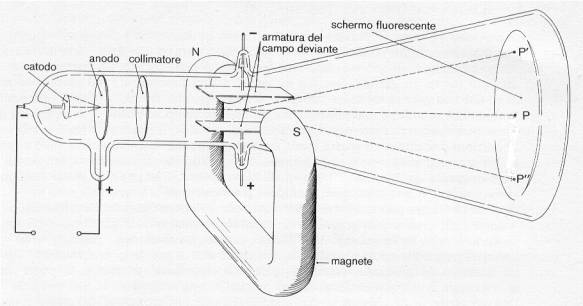
\includegraphics[width=\textwidth]{immagini/thompson.jpg} %immagine
\end{center}

Si ricordi $\vec F=q\left(\vec E+\vec \sigma \times \vec B \right)$.
\begin{enumerate}
\item In assenza di campo elettrico e magnetico:
\begin{equation}\begin{split}
v_x=\frac{l}{\Delta t}
\end{split}\end{equation}
\item Con campo elettrico:
\begin{equation}\begin{split}
eE_y=ma_y \Longrightarrow \\
v_y=\frac{eE_y}{m}\Delta t \Longrightarrow \\
\Delta y=\frac{eE_y}{2m}\left(\Delta t\right)^2=\frac{eE_y}{2m}\frac{l^2}{v^2_x}
\end{split}\end{equation}
\item Con campo elettrico e magnetico si ha $\vec F_e=e\vec E$ e $\vec F_m=-ev\vec B$:
\begin{equation}\begin{split}
F_y=0=eE_y-ev_xB_z \Longrightarrow \\
\Delta y=\frac{1}{2}a_y\left(\Delta t\right)^2=\frac{eE_y}{2m}\frac{l^2}{v^2_x}=\frac{e}{2m}l^2\frac{B^2_z}{E_y}
\end{split}\end{equation}
\end{enumerate}

Si può misurare quindi il rapporto carica-massa:
\begin{equation}\begin{split}
\frac{e^-}{m_e}=2\Delta y \frac{E_y}{B^2_zl^2}=1.76\cdot 10^{11} \textrm{C kg}^{-1}
\end{split}\end{equation}

\section{Esperimento di Millikan} %Esperimento di Millikan
Tutte le cariche misurate sono multiple intere di una carica elementare $e^-$ di massa $m_e=0.511$ MeV (pari a $9.1 \cdot 10^{-31}$ kg).

\begin{center}
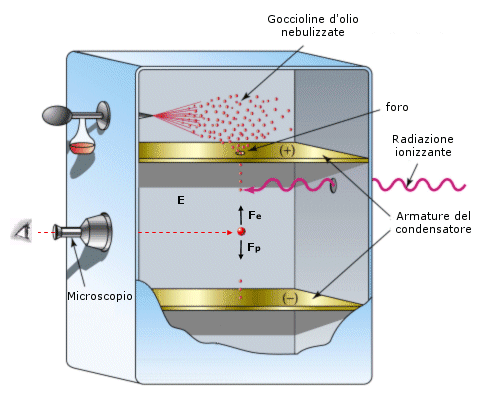
\includegraphics[width=\textwidth]{immagini/millikan.jpg} %immagine
\end{center}

In assenza di campo elettrico si ha che la goccia in caduta libera raggiunge una velocità limite $v_l$ . In quanto trascorso un transitorio iniziale la forza d'attrito viscoso viene bilanciata dalla forza peso. La velocità limite è misurabile sperimentalmente. La forza di attrito viscoso $F_v$ agente sulla goccia è data dalla legge di Stokes. Tale forza viene bilanciata dalla forza peso $F_g$ (trascurando la spinta di Archimede dell'aria).
\begin{equation}\begin{split}
\vec F=F_g-F_v=\frac{4}{3}\pi r^3\rho g-6\pi \eta r v_l=0 \Longrightarrow \\
r=3\eta ^{\frac{1}{2}} \left(\frac{v_l}{2\rho g}\right)^{\frac{1}{2}}
\end{split}\end{equation}

Viene applicata una differenza di potenziale nota $V_1-V_0$ tra le armature del condensatore a facce piane e parallele si genera un campo elettrico costante ed uniforme:
\begin{equation}\begin{split}
F_e=q\vec E \Longrightarrow \\
q\frac{V_1-V_0}{d}-\frac{4}{3}\pi r^3\rho g=6\pi \eta rv_s \Longrightarrow \\
q=\frac{d}{V_1-V_0}6\pi\eta r\left(v_s+v_l\right)=\frac{d}{V_1-V_0}18\pi\eta ^{\frac{3}{2}} \left(\frac{v_l}{2\rho g}\right)^{\frac{1}{2}} \left(v_s+v_l\right)
\end{split}\end{equation}

\section{Radiazioni} %Radiazioni
\begin{itemize}
\item $\alpha $: nuclei di elio, carica, si blocca con un foglio di carta: 

$m_\alpha =6.6\cdot 10^{-27}$ kg, $q_\alpha =3.2\cdot 10^{-18}$ C
\item $\beta $: elettroni, carica, si blocca con un foglio di alluminio o l'acqua:

${m_\beta =9.1\cdot 10^{-31}}$ kg, $q_\beta =1.6\cdot 10^{-18}$ C
\item $\gamma $: transizione di diversi stati del nucleo, non carica, si blocca con strati di piombo.
\end{itemize}

\section{Esperimento di Rutherford} %Esperimento di Rutherford
L'esperimento di Rutherford (anche detto esperimento di Geiger e Marsden) fu un esperimento effettuato per sondare la struttura dell'atomo eseguito da Hans Wilhelm Geiger e Ernest Marsden nel 1909, sotto la direzione di Ernest Rutherford. \textbf{Concepito per provare la validità del modello atomico di Thomson, detto modello a panettone (plum pudding model), diede dei risultati contrastanti rispetto a quel modello e portò alla concezione del modello atomico di Rutherford o modello planetario dell'atomo}.

\begin{center}
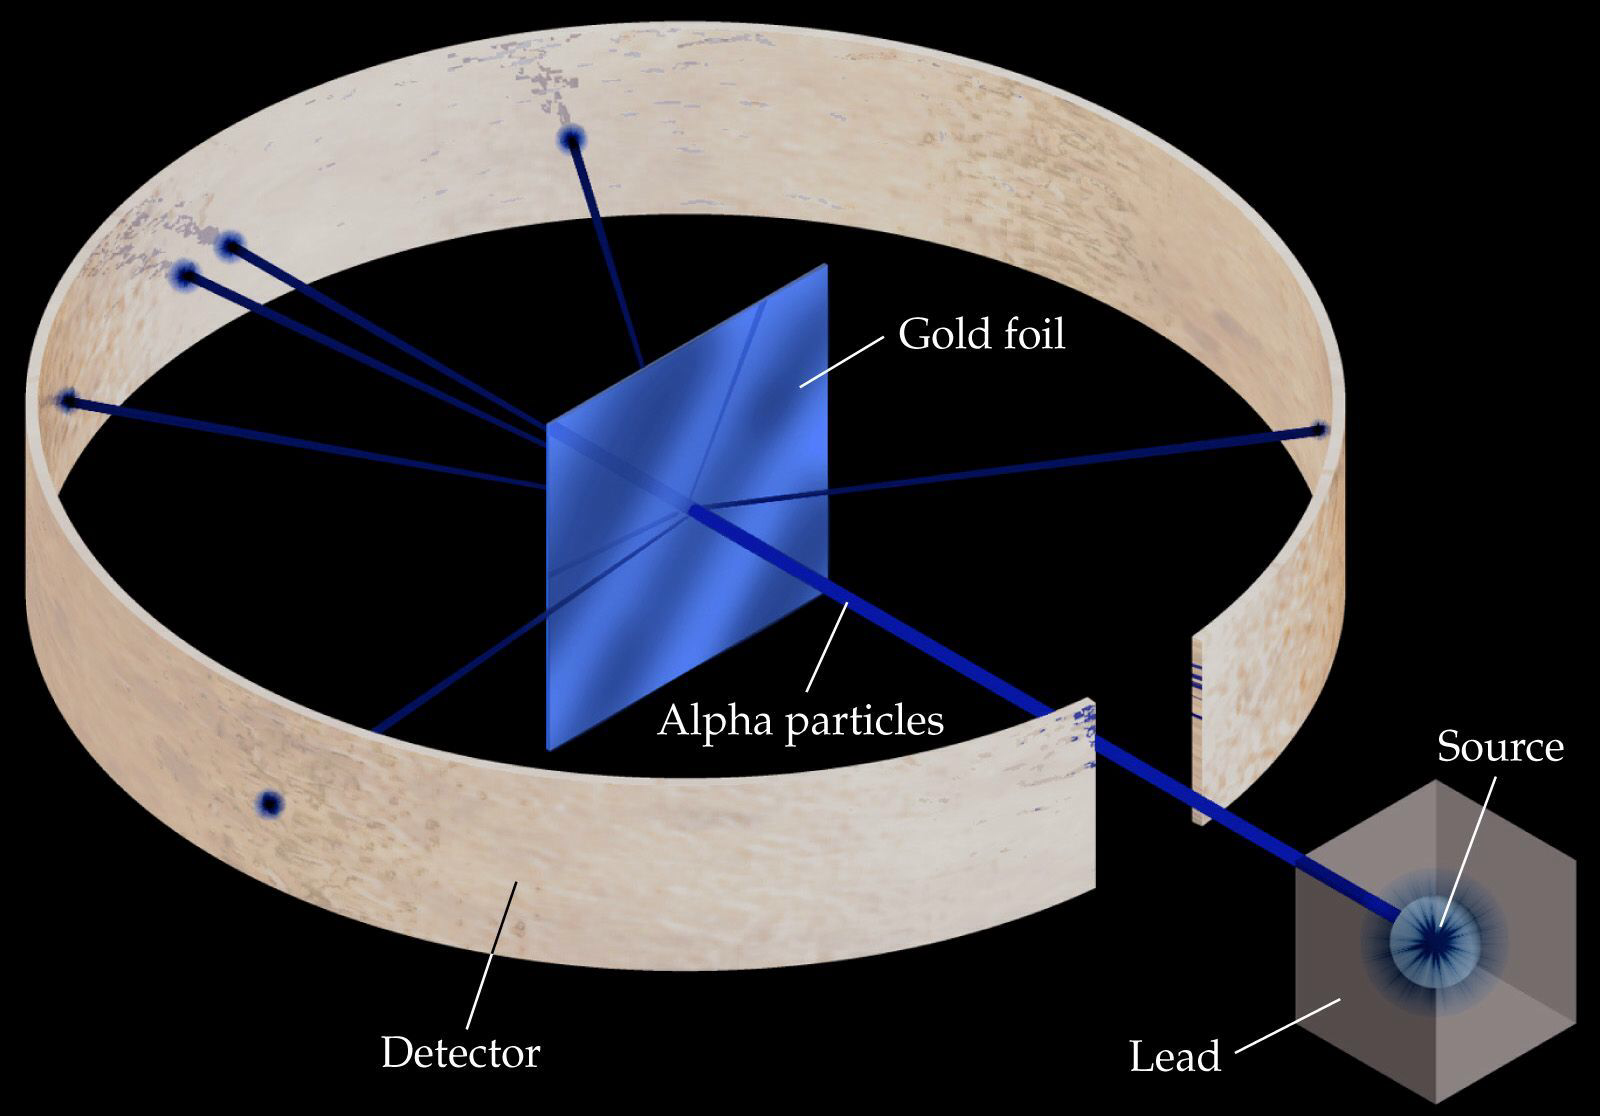
\includegraphics[width=\textwidth]{immagini/rutherford.jpg} %immagine
\end{center}

Un fascio di particelle $\alpha$ generate dal decadimento radioattivo di radio fu diretto ortogonalmente ad un foglio sottile d'oro. Il foglio d'oro era circondato da un foglio circolare ricoperto di solfuro di Zinco (\ce{ZnS}) usato come rivelatore: il solfuro di zinco emette scintille luminose quando viene colpito da particelle $\alpha$.
Secondo il modello di Thomson, allora maggioritario, le particelle $\alpha$ avrebbero dovuto attraversare il foglio d'oro venendo deflesse al più di pochi gradi, anche considerando la possibilità di diffusione multipla: misurando la deflessione delle particelle si potevano ricavare informazioni sulla distribuzione di carica elettrica all'interno dell'atomo. Tuttavia venne osservato che alcune particelle (1/8000) venivano riflesse ad angoli anche maggiori di 90º. 

\textbf{È un esperimento di scattering. Secondo il modello di Thomson ci si aspettava angoli di scattering molto piccoli ($\theta \sim 0$). Si trova però che alcune deflessioni sono anche di $\theta \sim 90º$}.
\begin{equation}\begin{split}
\Delta p=F \Delta t\sim \frac{1}{4\pi \epsilon _0}\frac{2Ze^2}{r^2}\frac{2r}{v}=\\
\frac{1}{\pi \epsilon _0}\frac{Ze^2}{r}\frac{1}{v} \Longrightarrow \\
\theta =\frac{\Delta p}{p}\sim \frac{1}{\pi \epsilon _0}\frac{Ze^2}{r}\frac{1}{v^2m}
\end{split}\end{equation}

Con questo modello non si capacita quindi la possibilità di angoli così grandi. \textbf{Rutherford perciò crea un nuovo modello e considera il nucleo puntiforme}.

\begin{equation}\begin{split}
V=\frac{zZe^2}{4\pi \epsilon _0r} \Longrightarrow \\
\vec F=-\vec \nabla V=\frac{zZe^2}{4\pi \epsilon _0}\frac{\vec r}{r^2}
\end{split}\end{equation}
\begin{equation}\begin{split}
\Delta p=\vec F\Delta t=2p\sin{\left(\frac{\theta }{2}\right)}.
\end{split}\end{equation}
Si ha la \textbf{distanza di massimo avvicinamento}:
\begin{equation}\begin{split}
b_0=\frac{p^2}{2m}=\frac{zZe^2}{4\pi \epsilon _0}\frac{2m}{\phi }
\end{split}\end{equation}

Si ricavano quindi la velocità:
\begin{equation}\begin{split}
\vec v=\frac{dr}{dt}\vec r+r\frac{d\phi }{dt}\vec n
\end{split}\end{equation}
e il momento angolare:
\begin{equation}\begin{split}
\vec L=m\vec v\times\vec r=r^2\frac{d\phi }{dt}\vec r\times \vec n
\end{split}\end{equation}
Si ha quindi la differenza di momento:
\begin{equation}\begin{split}
\Delta p=\\
\frac{zZe^2}{4\pi \epsilon _0}\int_{}^{}{\frac{m}{pb}\cos{\left(\phi \right)}\frac{d\phi }{dt} \textrm{d}t}=\\
2p\sin{\left(\frac{\theta}{2}\right)}=\\
\frac{zZe^2}{4\pi \epsilon _0}\frac{m}{pb}2\cos{\left(\frac{\theta }{2}\right)}
\end{split}\end{equation}
e quindi si può ricavare l'\textbf{angolo di deflessione}:
\begin{equation}\begin{split}
\tan{\left(\frac{\theta }{2}\right)}=\frac{b_0}{2b}
\end{split}\end{equation}

Nell'urto bisogna conoscere quante particelle passano oltre:
\begin{equation}\begin{split}
N_\theta \propto N_0nx\textrm{d}\Omega  \\
N_\theta = N_0 nx \frac{\textrm{d}\sigma\left(\theta\right)}{\textrm{d}\Omega}\textrm{d}\Omega
\end{split}\end{equation}
definendo la \textbf{sezione d'urto differenziale}:
\begin{equation}\begin{split}
\frac{\textrm{d}\sigma\left(\theta\right)}{\textrm{d}\Omega}=\frac{N\sigma}{N_0}\frac{1}{nx}\frac{1}{\sigma\Omega}
\end{split}\end{equation}
Misurato in m$^2$ sr$^{-1}$ o b sr$^{-1}$, avendo definito il $barn$=b=$10^{-28}$ m.

La \textbf{sezione d'urto totale} è:
\begin{equation}\begin{split}
\int {\frac{\textrm{d}\sigma}{\textrm{d}\Omega} \textrm{d}\Omega}=\sigma_{tot}
\end{split}\end{equation}

Per un nucleo per unità di area, la probabilità di scattering in $-\textrm{d}\theta$ è:
\begin{equation}\begin{split}
\frac{\textrm{d}\sigma}{\textrm{d}\Omega}=\\
\frac{2\pi b}{-2\pi \sin{\left(\theta\right)}}\frac{\textrm{d}b}{\textrm{d}\Omega}=-\frac{b\textrm{d}b}{\sin{\left(\theta\right)}\textrm{d}\theta}=\\
\frac{b^2_0}{16\sin{\left(\frac{\theta}{2}\right)}^4}
\end{split}\end{equation}
Essendo la corona circolare in uscita $\textrm{d}\Omega=-2\pi \sin{\left(\theta\right)} \textrm{d}\theta$, si ha $$b=\frac{b_0}{2}\tan{\left(\frac{\theta}{2}\right)}^{-1},$$ $$\textrm{d}b=-\frac{1}{2\sin{\left(\frac{\theta}{2}\right)}}\frac{b_0}{2}.$$

Rutherford interpretò i risultati sperimentali in un lavoro del 1911 intitolato "The Scattering of $\alpha$ and $\beta$ Particles by Matter and the Structure of the Atom" (La diffusione di particelle $\alpha$ e $\beta$ e la struttura dell'atomo.).
Nell'articolo \textbf{Rutherford rigettò definitivamente il "modello a panettone" di Thomson} dato che secondo quel modello né le particelle con carica negativa (ossia gli elettroni), né la distribuzione di carica positiva che doveva contenerli sarebbero stati in grado di produrre deflessioni così marcate.
Rutherford quindi \textbf{propose che la carica positiva dell'atomo fosse concentrata in uno spazio con un volume molto minore delle dimensioni atomiche}, in questo modo era possibile spiegare le deflessioni osservate. Questa concentrazione centrale di carica, successivamente denominata nucleo atomico, portava a concludere che \textbf{la maggior parte del volume atomico fosse costituito da spazio vuoto}. Infatti, dalla conservazione dell'energia cinetica, fu in grado di calcolare che il raggio della carica centrale negli atomi d'oro doveva essere più piccolo di $3.4\cdot 10^{-14}$ m, mentre l'atomo d'oro aveva un raggio noto di $1.5\cdot 10^{-10}$.

\section{Oltre Rutherford} %Oltre Rutherford
Aumentando l'energia non funziona così bene il modello e l'esperimento di Rutherford perché non si verificano più le ipotesi che il nuclo puntiforme abbia solo urti elastici senza interazione nucleare. Si capisce quindi che \textbf{il nucleo non è puntiforme}. I limiti si vedono in atomi più leggeri. \textbf{Aumentando l'energia non c'è solo un fenomeno elastico}. I nuclei hanno una densità uniforme, hanno pressoché una forma sferica. Il \textbf{raggio} è $R=r_0A^{\frac{1}{3}}$ con $r_0=1.1\sim 1.3$ fm. La \textbf{densità} è $$\rho\left(r\right)=\frac{\rho_0}{1-e^{\frac{r-R_0}{a}}}$$ con $\rho_0=0.1$ nc fm$^{-3}$, $a=0.4\sim 0.6$ fm e $R_0$ è il raggio quando si è a densità $\frac{\rho}{2}$ (nc: nucleoni, fm: fermi).

\subsection{Misura della massa del nucleo} %Misura della massa del nucleo
Facendo passare un nucleo all'interno di un condensatore carico si ritrova come nell'esperimento di Thomson ($p=Mv$):
\begin{equation}\begin{split}
\Delta p=F\Delta t=qE\frac{l}{v}=p\theta \\
\frac{\Delta p}{p}=\frac{q}{M}\frac{El}{v^2}\sim \theta \\
\Delta y=\frac{q}{2M}E\frac{l^2}{v^2}
\end{split}\end{equation}

Essendo presente il campo magnetico, si ha $\vec F=q\vec v\times \vec B$ e quindi:
\begin{equation}\begin{split}
\vec R=\frac{m\vec v}{q\vec B}.
\end{split}\end{equation}

Se sono presenti i campi magnetico e elettrico si ha:
\begin{equation}\begin{split}
q\vec E=q\vec v\vec B \Longrightarrow \frac{\vec E}{\vec B}=\vec v
\end{split}\end{equation}

\subsection{Spettrometro di massa} %Spettrometro di massa

\begin{center}
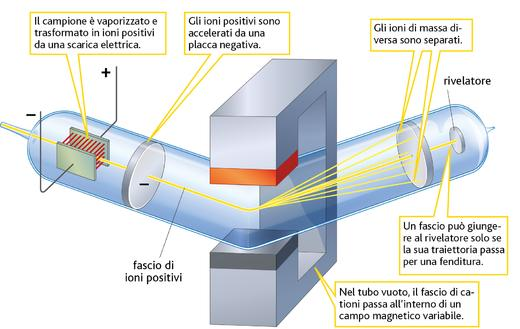
\includegraphics[width=5in]{immagini/spectrometer.jpg} %immagine
\end{center}

Grazie a questi accorgimenti si è creato lo \textbf{spettrometro di massa}. Si può misurare la massa atomica in questo modo, ma viene usato anche per separare gli isotopi.

\chapter{Il nucleo dell'atomo} %Nucleo dell'atomo
\section{Dimensioni}
\begin{itemize}
\item \textbf{Raggio}: $10^{-10}$ m
\item \textbf{Massa}: (in principio) $A$ protoni e $A-Z$ elettroni (dopo la meccanica quantistica) $A$ protoni e $A-Z=N$ neutroni
\item \textbf{Carica}: neutra
\end{itemize}
$Z$: numero di elettroni nell'atomo. $A$: numero di protoni nell'atomo. $N$: numero di neutroni nell'atomo.

Si indica con $\ce{_Z^AX}$ o $X\left(A,Z\right)$.

\section{Esperimento di Chadwick} %Esperimento di Chadwick

\begin{center}
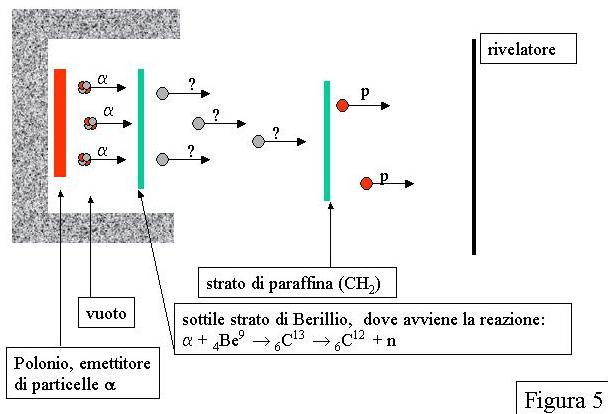
\includegraphics[width=5in]{immagini/chandwick.jpg} %immagine
\end{center}

\begin{equation}\begin{split}
\ce{^4_2He}+\ce{^9_4Be}\rightarrow \ce{^{13}_6C} \left(\textrm{instabile}\right)\rightarrow \ce{^{12}_6C}+n
\end{split}\end{equation}
Con $n$ neutrone.

La massa del protone è $938.2723$ \si{MeV/c^2}. La massa del neutrone è $939.505$ \si{MeV/c^2}.
\begin{itemize}
\item \textbf{Isotopi}: nuclei con \textbf{Z uguale e diverso A}, differiscono per il numero di neutroni.
\item \textbf{Isotoni}: nuclei con \textbf{N uguale ma Z diverso}, differiscono per il numero di elettroni.
\item \textbf{Isobari}: nuclei con \textbf{A uguale e diversi Z e N}, differiscono per il numero di elettroni e neutroni.
\end{itemize}

\section{Nucleo sferico - densità di massa} %Nucleo sferico - densità di massa
\begin{center}
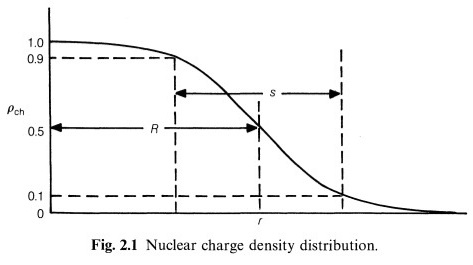
\includegraphics[width=\textwidth]{immagini/mass_density.jpg} %immagine
\end{center}

La distribuzione delle cariche è simile a quella in figura. Misurato con esperimenti di scattering di elettroni (gli elettroni interagiscono solo elettromagneticamente, non con interazione forte o debole).

\begin{equation}\begin{split}
\int{\rho_{ch}\left(r\right)\textrm{d}V}=4\pi\int{\rho_{ch}\left(r\right)r^2\textrm{d}r}=Z
\end{split}\end{equation}
${R_0}_{ch}=1.1\sim 1.2$ fm; ${R_0}_m=1.3\sim 1.4$ fm; $R=R_0A^\frac{1}{3}$; $V=\frac{4}{3}\pi R^3 \propto A$.

La superficie è definita come la regione in cui $\rho$ va dal $90\%$ al $10\%$. Ha dimensioni dell'ordine di circa $2.5$ fm.
\begin{equation}\begin{split}
\rho_m=\frac{m}{V}\\
m=Zm_p+Nm_n\propto A\\
m_n\simeq1.67\cdot 10^{-27}\textrm{ kg}
\end{split}\end{equation}
\begin{equation}\begin{split}
\rho\propto \frac{A}{A} \textrm{ sostanzialmente indipendente da A.}
\end{split}\end{equation}

\textbf{La materia nucleare è più densa di quella ordinaria}. Condizioni simili si hanno nelle stelle di neutroni.

\textbf{Distanza di separazione tra nucleoni}: $d$. \\
Per ogni nucleone il volume occupato sarà $d^3$. Il volume totale sarà quindi $$Ad^3=\frac{4}{3}\pi R_0A \longrightarrow d\simeq 1.6\sim 1.8 \textrm{ fm}.$$

Misurata \textbf{la massa effettiva di un nucleo, essa è diversa dalla somma $Zm_p+Nm_n$}. In generale:
\begin{equation}\begin{split}
M<Zm_p+Nm_n
\end{split}\end{equation} 
Ciò avviene perché c'è in gioco l'energia di legame. Se il nucleo è stabile è richiesta energia per costruire un nucleone:
\begin{equation}\begin{split}
\Delta M=M\left(A,Z\right)-Zm_p-\left(A-Z\right)m_n<0
\end{split}\end{equation}
\begin{equation}\begin{split}
\Delta mc^2=E_{\textrm{legame}}=B<0
\end{split}\end{equation}
\begin{equation}\begin{split}
M\left(A,Z\right)=Zm_P+\left(A-Z\right)m_n+\frac{B}{c^2}
\end{split}\end{equation}
(ridefinendo $B=\left[Zm_p+Nm_n-M\left(A,Z\right)\right]c^2>0$). \textbf{Tanto più è negativo B, tanto più il nucleo è stabile}.

In realtà spesso è difficile supporre il nucleo di tutti gli elettroni, perciò si definisce la massa atomica come:
\begin{equation}\begin{split}
M_{at}=M_{nucl}+Zm_e-\frac{B_{H}}{c^2}
\end{split}\end{equation}
considerando $\frac{B_{H}}{c^2}$ l'energia di legame degli elettroni presa positiva e prendendo $B=\left(ZM_H+Nm_n-M_{at}\right)c^2$ definito positivo, con $M_H$ la massa dell'idrogeno

\begin{center}\begin{tabularx}{2in}{XX}
\toprule
Nucleo & B \\
\midrule
$\ce{^2_1H}$ & $2.22$ MeV \\
$\ce{^3_1H}$ & $8.482$ MeV \\
$\ce{^3_2He}$ & $7.719$ MeV \\
$\ce{^4_2He}$ & $28.31$ MeV \\
$\ce{^{12}_6C}$ & $92.2$ MeV \\
$\ce{^{56}_{26}Fe}$ & $492.27$ MeV \\
$\ce{^{238}U}$ & $1803$ MeV \\
\bottomrule
\end{tabularx}\end{center}

\textbf{L'interazione nucleare è indipendente dalla carica}. Il fatto che B di $\ce{^3He}$ e $\ce{^3H}$ siano diverse dipende dall'interazione elettromagnetica. Il trizio $\ce{^3H}$ è più legato perché i due protoni in $\ce{^3He}$ si respingono un po'.

Oltre $A\simeq 12$, il rapporto $\frac{B}{A}$ è generalmente compreso tra circa 7.5 e 8.5 MeV, con un valore medio di circa 8 MeV. Per i nuclei molto leggeri, $\frac{B}{A}$ è significativamente inferiore ma con picchi pronunciati per A = \ce{^4He}, \ce{^8Be}, \ce{^{12}C}. l valore massimo è di circa 8.8 MeV nella regione $A\simeq 55-60$, ad esempio il \ce{^{56}Fe} con $\frac{B}{A}=8.79$ MeV. Oltre questo massimo il valore di $\frac{B}{A}$ diminuisce gradualmente.

\textbf{L'energia di legame va come A}, non con il numero di coppie di nucleoni. È un'indicazione del fatto che l'interazione nucleare è a corto raggio:

\begin{center}\begin{tabularx}{\textwidth}{XXXXXXX}
\toprule
& $\ce{^2H}$ & $\ce{^3H}$ & $\ce{^3He}$ & $\ce{^4He}$ & $\ce{^4Li}$ & \\
\midrule
B & $2.22$ & $8.482$ & $7.719$ & $28.31$ & $32$ & $\propto A$ \\
B/A & $1.11$ & $2.83$ & $2.57$ & $7.07$ & $5.35$ & costante (tranne che per nuclei molto leggeri) \\
Coppie & $1$ & $3$ & $3$ & $6$ & $15$ & $\propto \frac{A(A-1)}{2}$ \\
\bottomrule
\end{tabularx}\end{center}

Ciascun nucleone interagisce con quelli vicini, altrimenti si avrebbe un andamento proporzionale al numero di coppie e non con tutti. Invece si osserva una situazione compatibile con il corto raggio d'azione dell'interazione nucleare forte.

Per i \textbf{nuclei più leggeri} $Z \simeq N$. Per i \textbf{nuclei più pesanti} c'è un eccesso di neutroni $N>Z$. Aumentando i protoni c'è da bilanciare più repulsione coulombiana, per stabilizzare devono intervenire più neutroni.

È favorevole questo punto di vista dell'energia di legame cioè che un nucleo pesante si divida in due più leggeri che sono già legati $\rightarrow$ fissione. È anche favorevole unire due nuclei leggeri e formarne uno più pesante $\rightarrow$ fusione.

\section{Decadimenti} %Decadimenti
I nuclei stabili hanno un tempo medio di vita infinito (a meno di reazioni esterne).

Esistono nuclei instabili che decadono spontaneamente. Il decadimento è un processo statistico caratteristico di una vita media.
\begin{equation}
N(t)=N_0e^{\frac{t}{\tau}}
\end{equation}
Il numero $\Delta N$ di nuclei che decadono in $\Delta t$ dipende dal tempo e dal numero iniziale di nuclei presenti all'inizio dell'intervallo $\Delta t$.

\begin{equation}
\frac{\Delta N}{\Delta t}=-\lambda N \longrightarrow \frac{dN}{N}=-\lambda dt \longrightarrow \int_{N_0}^{N(t)}{\frac{dN}{N}}=-\lambda\int_{0}^{t}{\textrm{d}t}
\end{equation}
\begin{equation}
N(t)=N_0e^{-\lambda t}
\end{equation}
con $\lambda=\frac{1}{\tau}$ e $\tau$ rappresenta la \textbf{vita media}.

\textbf{Tempo di dimezzamento}, cioè tempo richiesto affinché $N(t)=\frac{N_0}{2}$:
\begin{equation}\begin{split}
t_{\frac{1}{2}}=\tau\ln{2}\simeq 0.7 \tau
\end{split}\end{equation}

\section{Stabilità nucleare} %Stabilità nucleare
Il nucleo è un sistema quantistico con diversi stati possibili. Quello a energia minima è quello fondamentale. Gli autostati dell'hamiltoniana sono discreti.

I nuclei che non decadono si distribuiscono così:

\begin{center}\begin{tabularx}{\textwidth}{XXXX}
\toprule
A & Z & N & Nuclei stabili\\
\midrule
pari & pari & pari & 165 \\
dispari & pari & dispari & 55 \\
dispari & dispari & pari & 50 \\
pari & dispari & dispari & 4 \\
\bottomrule
\end{tabularx}\end{center}
(Ricordando $Z$: numero di elettroni nell'atomo. $A$: numero di protoni nell'atomo. $N$: numero di neutroni nell'atomo).

La stabilità è associata con la parità del numero di protoni (Z) e neutroni (N). Sono le coppie di protoni e le coppie di neutroni a formare stabilità. La forza che tiene uniti i nuclei è più efficace tra coppie di protoni o coppie di neutroni. Si vede che \textbf{non fa tanta differenza se sono i protoni o i neutroni ad essere pari}. I dispari-dispari stabili sono solo nuclei leggeri: gli isotopi \ce{^7_3Li}, \ce{^{11}_5B} \dots

Possiamo scrivere per il nucleo una hamiltoniana:
\begin{equation}
\mathcal{H}=T+V_{\textrm{Coulomb}}+V_{\textrm{nucleare}}
\end{equation}
con $T=\sum^A_i{T_i}$ somma delle energie cinetiche dei nucleoni; $V_{\textrm{Coulomb}}=\sum^Z_{i,j;i\neq j}{V_i,j}$ tra coppie di protoni; $V_{\textrm{nucleare}}=\sum^Z_{i,j;i\neq j}{V_i,j}$ tra coppie di nucleoni.

L'equazione di Schrödinger $H\psi=E\psi$ diventa quindi $H\psi_n=E\psi_n$ per gli autostati con relativi livelli di energia. \textbf{Lo spettro è discreto}. Si ricavano anche i numeri quantici che descrivono proprietà del nucleo (momento angolare orbitale, spin). Ogni stato avrà un momento angolare totale $J$. Un'altra caratteristica è la parità dello stato $\Pi^+$ o $\Pi^-$: dipende dalla parità della funzione d'onda che descrive lo stato ($\Pi^+ \rightarrow \psi$ pari in $\vec r$).

\subsection{Gamma} %Gamma
\textbf{Si passa da uno stato nucleare eccitato meno legato a uno stato meno eccitato e più legato con emissione di energia}. Gli stati a energia superiore quella minima sono detti stati eccitati. Un decadimento da uno stato eccitato a quello fondamentale produce energia.

\subsection{Alpha} %Alpha
Nucleo iniziale non stabile $\longrightarrow$ $\ce{^4_2He}$ + nucleo stabile.
\begin{equation}\begin{split}
X\left(A,Z\right) \longrightarrow \ce{^4_2He}+Y\left(A-4,Z-2\right)
\end{split}\end{equation}
Se $M_X<M_{\alpha}+M_Y$ il nucleo è stabile.\\
Se $M_X>M_{\alpha}+M_Y$ può avvenire il decadimento con liberazione di energia.

\subsection{Beta} %Beta
\begin{equation}
X\left(A,Z\right) \longrightarrow 
\begin{cases}
Y\left(A,Z+1\right) \quad \beta^- & n\longrightarrow p+e^-+\bar\nu_e \\
Y\left(A,Z-1\right) \quad \beta^+ & p\longrightarrow n+e^++\nu_e
\end{cases}
\end{equation}
Un atomo diventa più stabile se un neutrone diventa un protone: \textbf{$\beta^-$}.\\
Un atomo diventa più stabile se un protone diventa un neutrone: \textbf{$\beta^+$}.

\section{Parità} %Parità
Per parità si intende la proprietà di un fenomeno di ripetersi immutato dopo un'inversione delle coordinate spaziali. Quando ciò avviene si dice che la parità si conserva, non si conserva in caso contrario.

Definiamo un \textbf{operatore parità P che ha la proprietà di riflettere ogni $r_i$ coordinate per l'origine}.

L'uniformità o stranezza di $\psi$ si mostra nella seguente equazione agli autovalori soddisfatta da tutti gli autostati di energia nucleare: $$P\psi(r_i)=P\psi(r_i)$$ dove $P=\pm 1$. Uno stato con $P = 1 (-1)$, si dice che abbia parità pari (dispari). Ciò significa che uno stato nucleare può essere etichettato con il suo spin e la sua parità: $J^P$. In particolare, gli stati fondamentali dei nuclei pari-pari si trovano sempre a $0^+$.

L'operatore di parità $P\psi(\vec r_i)=\pm\psi(\vec r_i)$ commuta con l'hamiltoniana:
\begin{equation}
[P,H]=0.
\end{equation}
\textbf{La parità è dunque una costante del moto, è conservata nei processi nucleari (interazione forte ed elettromagnetica)}. Per l'interazione debole invece la parità non è conservata. La parità si determina studiando la distribuzione di particelle in processi nucleari e può essere determinata sperimentalmente.

Alcune grandezze classiche che sono invarianti per inversione delle coordinate spaziali: $t$, il tempo in cui un evento avviene; $E$, l'energia di una particella; $P$, la potenza; $\vec L$, il momento angolare della particella (sia orbitale sia di spin); $\rho$, la densità di carica elettrica; $V$, il potenziale elettrico; $\vec B$, il campo magnetico; $\vec H$, il campo magnetico ausiliario; $\vec M$, la magnetizzazione; $\rho$, la densità di energia del campo elettromagnetico; $T_{ij}$, il tensore degli sforzi di Maxwell; $m$, la massa; $q$, la carica elettrica.

Alcune grandezze classiche che cambiano segno per inversione spaziale: $\vec x$, la posizione di una particella nello spazio tridimensionale; $\vec v$, la velocità di una particella; $\vec a$, l'accelerazione di una particella; $\vec p$, il momento lineare di una particella; $\vec F$, la forza su una particella; $\vec J$, la densità di corrente elettrica; $\vec E$, il campo elettrico; $\vec D$, l'induzione elettrica; $\vec P$, la polarizzazione elettrica; $\vec A$, il potenziale vettore elettromagnetico; $\vec S$, il vettore di Poynting.


\section{Momento angolare} %Momento angolare
Viene definito $\vec L=\vec r \times \vec p$ con l'operatore vettoriale $\hat {\vec l}=-i\hbar \hat{\vec r} \times \hat{\vec v}$. L'operatore ha tre componenti.

\subsection{Regole di commutazione} %Regole di commutazione
\begin{equation}\begin{split}
\left[\hat l_x,\hat l_y\right]=i\hbar \hat l_z\\
\left[\hat l_y,\hat l_z\right]=i\hbar \hat l_x\\
\left[\hat l_z,\hat l_x\right]=i\hbar \hat l_y
\end{split}\end{equation}

\subsection{Momento angolare intrinseco - spin} %Momento angolare intrinseco
Non ha un analogo classico. Viene definito come $\vec S$. Ha le tre componenti spaziali.

Si definisce allora il \textbf{momento angolare totale}:
\begin{equation}
\vec J=\vec l +\vec s.
\end{equation}
L'operatore vettoriale $\vec j$ avrà tre componenti con le stesse regole di commutazione del momento angolare: le tre componenti non commutano e quindi non possono essere diagonalizzate simultaneamente.
\begin{equation}
J^2=j^2_x+j^2_y+j^2_z
\end{equation}
\begin{equation}
\left[\hat J^2,\hat j_i\right]=0
\end{equation}
\begin{equation}\begin{split}
J^2\ket {j,m}=\hbar^2 j(j+1)\ket {j,m} \\
J_z \ket {j,m}=\hbar m \ket{j,m}
\end{split}\end{equation}
\textbf{Comunemente si dice che il sistema ha momento angolare $j$ intendendo però che l'autovalore è $\hbar j(j+1)$}.

Il caso particolare in cui lo spin è $\frac{1}{2}$ è molto interessante. Fissato $j$ si possono avere $2j+1$ possibili valori di $m$ tra $-j\le m \le +j$. Se $s=\frac{1}{2}$ si avrà $m_s=\pm\frac{1}{2}$.

Gli autostati $\ket{j,m}=Y_{l,m}(\theta,\phi)$ sono \textbf{armoniche sferiche}. Dalle proprietà di queste risulta la parità degli stati. La proprietà interessata è:
\begin{equation}
Y_{l,m}(\pi-\theta,\pi+\phi)=(-1)^lY_{l,m}(\theta,\phi)
\end{equation}
\textbf{lo stato pari è quindi quello con $l$ pari e lo stato dispari è quello con $l$ dispari}.

\subsection{Somma di momenti angolari} %Somma di momenti angolari
In generale vale $\vec j=\sum_i{\vec j_i}$. La somma segue le tipiche regole di commutazione. Il valore di $\vec j$ può andare da $\left|j_1-j_2\right|\le j\le\left|j_1+j_2\right|$. \textbf{I $j$ dei singoli nucleoni possono essere semi interi mentre il $j_{totale}$ del nucleo può essere sia intero sia semi-intero a seconda che ci siano un numero pari o dispari di nucleoni}.

Quando si definisce uno stato di un nucleo, lo si definisce come $\Psi_{J,M}$.
\begin{equation}\begin{split}
J^2\Psi_{J,M}=\hbar^2J(J+1)\Psi_{J,M}\\
J_z\Psi_{J,M}=\hbar M\Psi_{J,M}
\end{split}\end{equation}
con $2J+1$ valori di $M$ e con $-J\le M\le+J$.

Con \textbf{A pari} si possono ottenere valori di $J$ interi. Nei nuclei con \textbf{N pari e Z pari (pari-pari)} lo stato fondamentale ha $J=0$ ed è uno stato con \textbf{parità positiva}. Nei nuclei con \textbf{parità dispari, $J$ è semi-intero}.

Vengono definiti:
\begin{equation}
\vec \mu_l=-\frac{e}{2m}\vec l \quad \textrm{\textbf{momento magnetico orbitale}}
\end{equation}
\begin{equation}
\mu_B=\frac{e\hbar}{2m} \quad \textrm{\textbf{magnetone di Bohr}}
\end{equation}
\begin{equation}
\hat{\mu_S}=-\frac{e}{2m}g\hat S \quad \textrm{\textbf{momento magnetico di spin}}
\end{equation}
con $g\sim 2$.

Per l'elettrone $S=\frac{1}{2}$, $m_S=\frac{1}{2}$: $\mu_S=-g\frac{e}{2m}S_z$. Con $S_z=\frac{\hbar}{2}$:
\begin{equation}
\mu_S=-\frac{1}{2}g\frac{e\hbar}{2m_e}=-\frac{1}{2}\mu_B.
\end{equation}

Per i nucleoni:
\begin{equation}
\begin{split}
\vec{\mu_{P,N}}_S=g_{P,N}\frac{e}{2m_{P,N}}\vec S_{P,N}\\
\vec{\mu_{P,N}}_S=\frac{1}{2}g_{P,N}\mu_N
\end{split}
\end{equation}
con $\mu_N=\frac{e\hbar}{2m_{P,N}}$ \textbf{magnetone nucleare}. Considerando $g_P=5.58$ e $g_N=-3.8262$. I momenti magnetici dei nucleoni sono 3 ordini di grandezza più piccoli di quelli dell'elettrone, per via della massa molto più piccola di quest'ultimo.

Le anomalie rispetto ai valori misurati sono dovute alla struttura interna dei nucleoni.

Per un nucleo si può definire un \textbf{momento magnetico totale}:
\begin{equation}
\vec \mu_J=g_J\frac{e}{2m_{\textrm{nucleone}}}\vec J=g_J\mu_N\vec J
\end{equation}
con $\mu_N= 5.0507 \cdot 10^{-27} \si{\joule\per\tesla}$.

\section{Momento magnetico di quadrupolo} %Momento magnetico di quadrupolo
La quantità che misura meglio la forma della simmetria e mostra quanto i nuclei deviano dalla simmetria sferica è:
\begin{equation}\begin{split}
Q_0=\int{\rho_n\left(\vec r\right)\left(3z^2-r^2\right)\textrm{d}V}=Z\left(3\left\langle z^2 \right\rangle\left\langle r^2 \right\rangle\right)
\end{split}\end{equation}
e si misura in m$^2$ o b$^2$ (b=barn).

Se si ha la forma sferica si ha che le medie quadrate di x, y e z sono uguali tra loro.
\begin{itemize}
\item $Q=0$: $\left\langle z^2 \right\rangle=\frac{1}{3}\left\langle r^2 \right\rangle$
\item $Q>0$: $\left\langle z^2 \right\rangle>\frac{1}{3}\left\langle r^2 \right\rangle$
\item $Q<0$: $\left\langle z^2 \right\rangle<\frac{1}{3}\left\langle r^2 \right\rangle$
\end{itemize}
Il valore di $Q$ varia da $-1\sim+8$ b.

\begin{center}
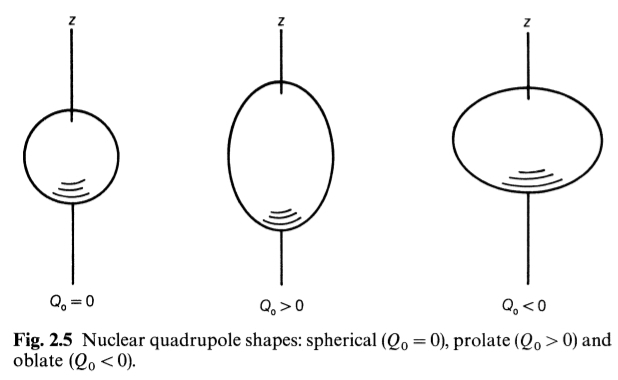
\includegraphics[width=\textwidth]{immagini/quadrupole.jpg} %immagine
\end{center}

\chapter{Interazione nucleare} %Interazione nucleare
Si ha la forza di interazione $\vec F\left(\vec r\right)=-\vec \nabla V\left(\vec r\right)$ intendendo $V$ come potenziale nucleare. In fisica nucleare si parla di \textbf{interazione a due corpi}: interazioni tra due nucleoni. $\vec r$ è la distanza tra i due nucleoni.

Essendo $B$ l'energia di legame, in funzione di $A$ si ha che essa è proporzionale a questa: \textbf{per togliere un nucleone devo dare la stessa energia}.
\begin{equation}\begin{split}
\frac{B}{A}\sim \textrm{const}
\end{split}\end{equation}

L'interazione nucleare va come $\frac{1}{r}$. \textbf{L'interazione è a corto raggio d'azione}. Il numero di nucleoni di cui un nucleone sente l'interazione rimane grosso modo sempre lo stesso.

Il \textbf{range} delle forze nucleari è intorno ai $2$ fm. Il \textbf{volume} $\propto R^3=A$ (essendo $R=r_0A^{\frac{1}{3}}$) considerando $A$ come il numero di nucleoni.

Per distanze molto piccole, l'attrazione da attrattiva diventa repulsiva (più forte dell'interazione nucleare normale attrattiva).

\section{Potenziali a basse energie} %Potenziali a basse energie
Si prende $V\left(\vec r\right)$ a buca quadrata, o gaussiano $V\left(\vec r\right)=v_0e^{-\left(r/r_0\right)^2}$, o $V\left(\vec r\right)=-v_0e^{-r/r_0}$, o $V\left(\vec r\right)=-v_0\frac{e^{-r/r_0}}{r/r_0}$. 

\textbf{Ciò che conta è che dipenda da due paramentri}. $v_0$ è dell'ordine $10\sim 35$ MeV.

La prima interazione nucleare è quella del \textbf{deutone}:
\begin{equation}\begin{split}
\textrm{spettro } n-p \Longrightarrow \ce{_1^2H}
\end{split}\end{equation}
esso ha le caratteristiche:
\begin{enumerate}
\item Energia di legame: $B=-2.22$ MeV
\item $J=1^+$
\item $\mu=0.84 \mu_N$
\item $Q=0.88\cdot 10^{-31}$ m (non è perfettamente sferico)
\end{enumerate}

Si parte dall'equazione di Scrhödinger $H\psi =E\psi $ per due nucleoni con $$H=\frac{p^2}{2m}+V\left(\vec r\right).$$ La massa ridotta è $\mu=\frac{m_pm_n}{m_p+m_n}\simeq\frac{m}{2}$. \textbf{Si utilizzano le coordinate sferiche} e si ottiene:
\begin{equation}\begin{split}
\left[-\frac{\hbar }{2\mu}\nabla ^2+V\left(\vec r\right)\right]\psi =E\psi 
\end{split}\end{equation}

\begin{equation}\begin{split}
p^2=p_r^2+\frac{l^2}{\vec r^2}
\end{split}\end{equation}
con $p_r=\frac{\hbar }{i}\left(\frac{\partial }{\partial r^2}+\frac{1}{r}\right)$ e $l$ il momento angolare.

In coordinate sferiche polari si ha quindi:
\begin{equation}\begin{split}
H=\frac{p_r^2}{2m}+\frac{l^2}{2m\bar r}+V\left(\vec r\right)
\end{split}\end{equation}
e si ha $\left[H,l^2\right]=0$.

Risolvendo agli autovalori si ha:
\begin{equation}\begin{split}
\psi _{l,n}\left(r,\theta,\phi\right)=Y_{l,m}\left(\theta,\phi\right)R_{n,l}\left(\theta,\phi\right)
\end{split}\end{equation}
e si riscrive l'equazione di Scrhödinger:
\begin{equation}\begin{split}
\left[-\frac{\hbar ^2}{2m}\frac{\textrm{d}^2}{\textrm{d}r^2}+l\left(l+1\right)\frac{\hbar ^2}{2m^2}+V\left(\vec r\right)-E\right]u\left(r\right)=0
\end{split}\end{equation}
essendo $R=\frac{u}{r}$, $n=1,2,3\dots$ numero quantico fondamentale, $l=1,2,3\dots n-1$ momento angolare orbitale, $-l\le m\le l$.

Ci si pone \textbf{nel caso di $l=0$}, quindi in uno stato $s$, e si risolve la nuova equazione:
\begin{equation}\begin{split}
\left[-\frac{\hbar ^2}{2m}\frac{\textrm{d}^2}{\textrm{d}r^2}+V\left(\vec r\right)-E\right]u\left(\vec r\right)=0.
\end{split}\end{equation}
Ci si pone quindi \textbf{con un potenziale a buca quadrata} e si ha:
\begin{itemize}
\item Nella regione $V<a$:
\begin{equation}\begin{split}
-\frac{\hbar ^2}{2m}\frac{\textrm{d}^2u}{\textrm{d}r^2}=\left(V_0-B\right)u
\end{split}\end{equation}
ricavando la \textbf{soluzione generale}:
\begin{equation}\begin{split}
u=A\sin{\left(\alpha r\right)}+C\cos{\left(\alpha r\right)}=A\sin{\left(\alpha r\right)}
\end{split}\end{equation}
con $\alpha=\sqrt{\frac{2\mu\left(V_0-B\right)}{\hbar ^2}}$.

\item Per $V>a$ si ha:
\begin{equation}\begin{split}
u=De^{-\beta r}+Fe^{\beta r}=De^{-\beta r}
\end{split}\end{equation}
con $\beta=\sqrt{\frac{2mB}{\hbar ^2}}$.

\item Per $V=a$ si ha infine:
\begin{equation}\begin{split}
A\sin{\left(\alpha r\right)}=De^{-\beta r} \\
\Longrightarrow \tan{\left(\alpha a\right)}^{-1}=-\frac{\beta}{\alpha}.
\end{split}\end{equation}
Nel caso in cui $B=0$
\begin{equation}\begin{split}
\alpha a=n\frac{\pi }{2} \quad \textrm{con } n=1,3,5\dots\\
\Longrightarrow v_0a=10^{-28} \textrm{MeV m}^2
\end{split}\end{equation}
\end{itemize}
Ricordando sempre che $B$ è l'energia di legame del deutone e avendo preso $\alpha a=\frac{\pi }{2}$.

Considerando $\beta^{-1}=4.3$ fm si ha il raggio del deutone per cui $V\rightarrow 0$.

L'\textbf{energia totale nucleare} è:
\begin{equation}\begin{split}
H=\sum{T_i}+\sum{V_{i,j}^N\left(r_{i,j}\right)}+\sum{V_{i,j}^C\left(r_{i,j}\right)}
\end{split}\end{equation}

\begin{equation}\begin{split}
J=1 \Longrightarrow \vec J=\vec L+\vec S \\
S=\vec s_1+\vec s_2
\end{split}\end{equation}

Abbiamo visto che la funzione d'onda del deutone, assumendo un potenziale a forma di buca, ha la forma:
\begin{equation}\begin{split}
V=
\begin{cases}
A\sin\left(\alpha r\right) & r\le A \\
De^{-\beta r} & r>A 
\end{cases}
\end{split}\end{equation}

\begin{center}
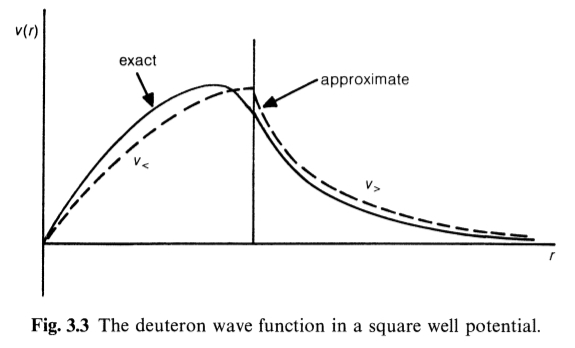
\includegraphics[width=5in]{immagini/internucleon-potential.jpg} %immagine
\end{center}

Quest'ultima figura dà una scala per la distanza a cui la funzione d'onda deutone muore lontano: dà un'indicazione della dimensione del deutone ed è chiaramente molto più grande del range approssimativo del potenziale internucleare ipotizzato, vale a dire 2 fm. La curva approssimativa si riferisce alla soluzione approssimata, mentre la curva esatta si riferisce alla soluzione esatta di questa equazione ed è stata presa per essere 2 fm. È chiaro che \textbf{il neutrone e il protone nel deutone spendono molto del loro tempo al di fuori del range di potenziale internucleare}.

Un ulteriore conclusione si può trarre dai dati considerati finora, e cioè che il potenziale internucleare deve essere dipendente dallo spin. Questo segue perché nello stato fondamentale del deutone il neutrone e il protone sono in uno stato di tripletto di spin (J = 1) e non ci sono stati eccitati. Se il potenziale era indipendente degli orientamenti di spin relativi del neutrone e del protone uno stato di singoletto del deutone (J = 0) esisterebbe con la stessa energia, come lo stato di tripletto. Questo non è osservato e l'assenza di un tale stato comporta che \textbf{il potenziale del singoletto è certamente più debole rispetto al potenziale di tripletto}.

Se si ha quindi $J=1$ e si possono avere i casi:
\begin{itemize}
\item $L=0 \Longrightarrow s=1 \Longrightarrow$ orbitale $\ce{^3s_1}$ pari
\item $L=1 \Longrightarrow s=0,1$ e $p=1 \Longrightarrow $ orbitali $ \ce{^1p_1}; \ce{^3p_1}$ dispari (va scartata)
\item $L=2 \Longrightarrow $ orbitale $ \ce{^3d_1}$ pari
\end{itemize}

\begin{equation}\begin{split}
\psi \left(s,d\right)=c_1\psi \left({^3s_1}\right)+c_2\psi \left({^3d_1}\right)
\end{split}\end{equation}

Si aggiunge un termine tensoriale $$f_t\left(r\right)\left[3\frac{\vec S_1\cdot \vec r\cdot \vec S_2\cdot \vec r}{r^2}-\vec S_1\bar S_2\right]$$ e si ha:
\begin{equation}\begin{split}
V=V_c+V_s+V_t=\\
=f_c\left(r\right)+f_s\left(r\right)\vec S_1\cdot \vec S_2+f_t\left(r\right)\left[3\frac{\vec S_1\cdot \vec r\cdot \vec S_2\cdot \vec r}{r^2}-\vec S_1\bar S_2\right]\\
\textrm{termine centrale + termine di spin + termine tensoriale}
\end{split}\end{equation}
\textbf{Per gli spin è energeticamente più favorevole essere paralleli}.

Ai termini di energia più alta si deve aggiungere anche un \textbf{termine di spin-orbita} $$f_{ls}=\vec L\cdot \vec S$$ con $\vec L=\frac{1}{2}\left(\vec r_1+\vec r_2\right)\times \left(\vec p_1-\vec p_2\right)$.

\textbf{L'interazione nucleare è indipendente dalla carica.}

Dal momento in cui \textbf{protoni e neutroni} si comportano nello stesso modo \textbf{si possono considerare come se fossero la stessa particella nei due stati di carica}.

Considerando \textbf{nuclei speculari}, essi \textbf{hanno spettri simili}.

\subsection{Fotone $\gamma$} %Fotone
Ha massa nulla. $E=pc$. $c=\lambda\nu$. $E=h\nu$. $p=\frac{h}{\nu}$. In meccanica quantistica se si fa lo scattering non compare il campo elettromagnetico, ma il fotone, e si ricava:
\begin{equation}\begin{split}
V=\frac{e^2}{4\pi\varepsilon_0r}
\end{split}\end{equation}

\subsection{Nucleoni e pione} %Nucleoni e pione
Il range finito nel caso nucleare avviene attraverso una particella simile al fotone, ma con massa diversa da quella nulla:
\begin{equation}\begin{split}
N\rightarrow N+\pi
\end{split}\end{equation}
con $\pi$ si intende il pione.

Considerando il principio di Heisenberg $\Delta E\Delta t\ge \hbar $ si ha che \textbf{il pione è una particella virtuale che compare nel tempo}
\begin{equation}\begin{split}
\Delta t\sim \frac{\hbar }{m_\pi c^2}
\end{split}\end{equation}
per ovviare il problema della conservazione dell'energia.

Il \textbf{range dell'interazione} è quindi:
\begin{equation}\begin{split}
c\Delta t \sim \frac{\hbar }{m_\pi c}
\end{split}\end{equation}
e quindi si ricava la \textbf{massa del pione} di circa $140$ MeV.

\chapter{Modelli nucleari} %Modelli nucleari
Basandosi sui dati sperimentali si può sostituire un potenziale fenomenologico per l'interazione nucleare. Un approccio alternativo è la teoria mesonica, analoga al caso elettromagnetico.

\section{Idea di Yukawa} %Idea di Yukawa
Essendo $m\neq 0$ il raggio è finito: nasce l'idea di pione. Dalla riduzione non relativistica si ottiene il potenziale. \textbf{Il pione esiste come $\pi^+$, $\pi^-$, $\pi^0$}. Tenuto conto della carica si capiscono anche i processi di scambio di carica.

Utilizzando il formalismo dell'isospin, si ottiene il potenziale di scambio di pioni, che è il termine relativamente a lungo raggio del potenziale nucleare. Per ottenere il core repulsivo, o ad esempio la parte di spin orbita, bisogna pensare a processi più complessi con più pioni. Restano comunque alcuni parametri da cui dipendono i risultati: costanti di accoppiamento e intensità della forza. 
\textbf{Scambiando particelle pesanti si avrà accesso a regioni più a corto raggio}.

Di fatto sono stati proposti diversi potenziali che descrivono bene il sistema a due nucleoni.

Il problema ora è mettere il potenziale nell'equazione di Schrödinger per risolvere il problema nucleare (sistema di $N_A$ particelle). Servono tecniche a molti corpi ma questo è problema proibitivo. Si fanno perciò delle semplificazioni, cioè i modelli nucleari. Ci si concentra su delle proprietà particolari. \textbf{Non ci si aspetta che un solo modello spieghi bene tutte le proprietà}.

\section{Modello a particelle indipendenti} %Modello a particelle indipendenti
\textbf{Il sistema nucleare è la somma delle proprietà dei singoli nucleoni, trascurando l'interazione}. Ciascun nucleone sente un campo medio. L'hamiltoniana sarà la somma delle singole hamiltoniane:
\begin{equation}
\mathcal{H}=\sum^A_i\mathcal{H}_i=\sum^A_i{T_i+U_i}
\end{equation}
Ciascun nucleone conserva la sua indipendenza: non vede gli altri.

\section{Modello a goccia di liquido} %Modello a goccia di liquido
Modello fenomenologico. \textbf{Spiegazione dell'energia di legame come differenza tra la somma delle masse di nucleoni e quella del nucleo}. 

Questo modello consente una panoramica generale delle masse, energie di legame e stabilità dello spettro completo dei nuclei ottenuti. Si basa sull'idea semplice che un nucleo si comporta in alcuni aspetti come una goccia di liquido.

Per esempio, le forze intermolecolari sono relativamente di piccolo range in modo che la quantità di energia necessaria per far evaporare una data massa di liquido da una goccia (calore latente di vaporizzazione) sia indipendente dalla dimensione della goccia come l'energia di legame di un nucleone è approssimativamente indipendente da A.

Si basa sull'\textbf{idea che il nucleo si comporti come una goccia di liquido per certe proprietà}:
\begin{itemize}
\item \textbf{Densità}: 
\begin{center}
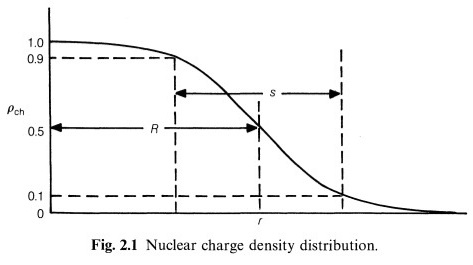
\includegraphics[width=3.5in]{immagini/mass_density.jpg} %immagine
\end{center}
\item \textbf{Volume}: Si suppone avere la forma sferica $V=\frac{4}{3}\pi R^3$, $R=r_0A^{\frac{1}{3}}$. Nei liquidi il volume aumenta con il numero delle molecole:
\begin{equation}
V\propto A.
\end{equation}
\item \textbf{Calore latente di vaporizzazione}: è indipendente dalle dimensioni della goccia, come l'energia che lega un nucleone al nucleo non dipende dalle dimensioni del nucleo.
\item \textbf{Energia di legame}: Nel liquido l'energia di legame aumenta appunto con il numero delle molecole:
\begin{equation}
\frac{B}{A}\sim \textrm{const} \Longrightarrow B\propto A.
\end{equation}
\begin{center}
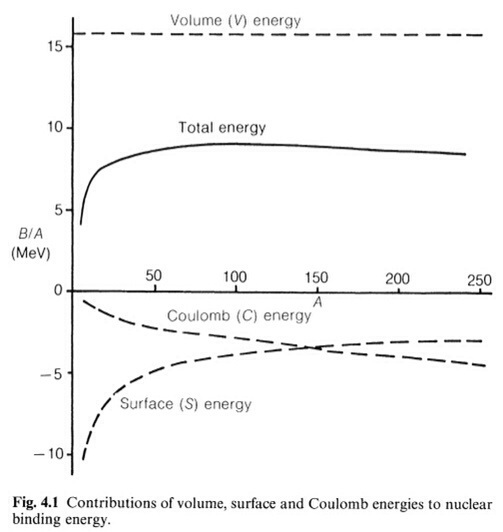
\includegraphics[width=4in]{immagini/density_liquid.jpg} %immagine
\end{center}
\end{itemize}

Consideriamo un nucleo con A-Z neutroni e Z protoni. I \textbf{contributi alla massa del nucleo} sono:
\begin{equation}
M(Z,A)=Zm_p+(A-Z)m_n-a_{V}A
\end{equation}
il primo termine è la massa dei protoni, il secondo quella dei neutroni e l'ultimo termine è l'\textbf{energia di legame di volume} proporzionale ad A (potenziale attrattivo a corto raggio).

Bisogna tener conto anche il contributo delle interazioni sulla superficie: esso è tanto più importante quanto più piccolo è A ($R^2\propto A^{\frac{2}{3}}$). \textbf{I nucleoni sulla superficie} interagiscono solo con il nucleoni all'interno: \textbf{subiscono meno attrazione}.

Correggiamo il termine di volume con qualcosa di positivo, cioè il \textbf{termine di superficie}: $$+a_SA^{\frac{2}{3}}.$$

C'è poi il \textbf{potenziale coulombiano per i soli protoni} (repulsivo): $$+a_C\frac{Z^2}{A^{\frac{1}{3}}}.$$

C'è un \textbf{termine di asimmetria} che dipende dalla differenza tra numero di neutroni e protoni. Per nuclei piccoli $N\simeq Z$, per nuclei grandi $N>Z$ (se Z è grande il termine coulombiano è grande, e quindi perché il nucleo sia stabile ci vogliono più neutroni): $$+a_{AS}\frac{(A-2Z)^2}{A}.$$

La stabilità dei nuclei dipende anche dal fatto che ci siano un numero di particelle dello stesso tipo. C'è un termine per tener conto di questi casi cioè il \textbf{termine di pairing}: 
\begin{equation*}
\delta(A,Z)=
\begin{cases}
-a_{(0-E)}A^{-\frac{3}{4}} & \textrm{pari-pari} \\
0 & \textrm{dispari-dispari} \\
+a_{(0-E)}A^{-\frac{3}{4}} & \textrm{dispari-pari, pari-dispari}
\end{cases}
\end{equation*}

In definitiva si ha quindi:
\begin{equation}
M(A,Z)=Zm_p+(A-Z)m_n-a_{V}A+a_SA^{\frac{2}{3}}+a_C\frac{Z^2}{A^{\frac{1}{3}}}+a_{AS}\frac{(A-2Z)^2}{A}+\delta(A,Z).
\end{equation}
Sperimentalmente si è ottenuto:
\begin{equation}
\begin{cases}
a_l=15.58\\
a_S=18.3\\
a_C=0.71\\
a_{AS}=23.7\\
a_{0-E}=3.4
\end{cases}
\end{equation}

Si ottiene con l'\textbf{energia di legame}
\begin{equation*}
B=\left[Zm_p+(A-Z)m_n-M(A,Z)\right]c^2
\end{equation*}
(se c'è anche l'elettrone c'è da aggiungere $Zm_e$).\\
Trascurando il termine di pairing si ha:
\begin{equation}
\begin{split}
B\simeq \left[a_{V}A-a_SA^{\frac{2}{3}}-a_C\frac{Z^2}{A^{\frac{1}{3}}}-a_{AS}\frac{(A-2Z)^2}{A}\right]c^2\\
\frac{B}{A}\simeq \left[a_{V}-a_SA^{-\frac{1}{3}}-a_C\frac{Z^2}{A^{\frac{4}{3}}}-a_{AS}\frac{(A-2Z)^2}{A^2}\right]c^2
\end{split}
\end{equation}
\textbf{Il contributo principale è effettivamente indipendente da A}. Gli altri contributi forniscono una spiegazione dell'andamento generale che funziona abbastanza bene.

Si fa poi $\frac{\partial M}{\partial Z}$ (trascurando il termine di pairing) e lo si pone uguale a zero. Si ottiene:
\begin{equation}
\frac{\partial M}{\partial Z}=0 \Longrightarrow Z=\frac{A}{1.37+0.0015\cdot A^{\frac{2}{3}}}
\end{equation}
che fornisce per un certo A lo Z che forma il nucleo più stabile. Si vede che $Z\sim \frac{A}{2}$ per A grande.

Ad esempio $\ce{^{16}_8O}$ con $A=16$ e $Z=8$: $B(16,8)=-122.81$ \si{MeV}; $B/A\simeq 7.7$ \si{MeV}.
\begin{center}\begin{tabularx}{\textwidth}{XXX}
\toprule
\midrule
\ce{^{12}_{6}C} & $B=-97.8$ \si{MeV} & $\frac{|B|}{A}=7.3$ \si{MeV}\\
\ce{^{14}_{6}C} & $B=-103.76$ \si{MeV} & $\frac{|B|}{A}=7.4$ \si{MeV}\\
\ce{^{56}_{26}Fe} & $B=-487.92$ \si{MeV} & $\frac{|B|}{A}=8.4$ \si{MeV}\\
\bottomrule
\end{tabularx}\end{center}

\section{Modello a shell - particelle indipendenti} %Modello a shell
\textbf{Sperimentalmente si osserva che quando si ha un certo numero "magico" di protoni o di neutroni, cioè 2, 8, 20, 28, 34, 50, 82, 126, si ottengono particolari proprietà di stabilità.}

I nuclei doppiamente magici sono particolarmente stabili (con un numero magico di protoni e uno di neutroni) ed esempio \ce{^{4}_{2}He}, \ce{^{40}_{20}Ca}, \ce{^{208}_{82}Pb}, \ce{^{10}_{8}O}.

Gli effettivi valori di $|B|$ sono più alti di quelli predetti dal modello a goccia di liquido, e si formano molti isotoni e/o isotopi stabili, per i nuclei con almeno un numero magico. I nuclei con numeri magici sono più abbondanti in natura. Per i nuclei doppiamente magici il primo stato eccitato è ad un'energia molto più elevata dei vicini (lo stato fondamentale è stabile). \textbf{I momenti di quadrupolo elettrico vanno a zero per i numeri magici}.

L'\textbf{energia di separazione} è l'energia necessaria per estrarre il nucleone meno legato da un nucleo:
\begin{equation}
S_n(N,Z)=B(N,Z)-B(N-1,Z) \quad \textrm{energia di separazione per un neutrone}
\end{equation}
\begin{equation}
S_p(N,Z)=B(N,Z)-B(N,Z-1) \quad \textrm{energia di separazione per un protone}
\end{equation}
Questa energia \textbf{ha dei massimi se i nuclei hanno numeri magici}.

Ci sono analogie con la ionizzazione dell'atomo per quanto riguarda il rapporto tra energie di separazione e numeri magici.

Nell'atomo gli elettroni hanno stati discreti, potenziale coulombiano, gli stati sono autostati dell'hamiltoniana e del momento angolare: si considerano perciò gli orbitali. Avviene un riempimento successivo dei livelli energetici del potenziale coulombiano. Per ogni livello c'è una degenerazione, più elettroni possono stare sullo stesso livello. Per il principio di esclusione di Pauli possono starcene 2 per ogni livello di energia; si hanno quindi un valore di $l$ e $2(2l+1)$ stati occupati da due elettroni. Per analogia si è sviluppato il modello a shell nucleare. \textbf{Al riempimento di certi livelli corrispondono i numeri magici}.

\begin{center}
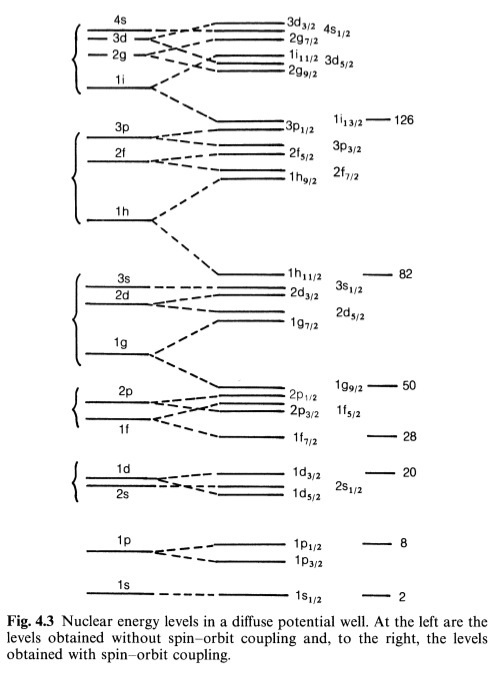
\includegraphics[width=4.3in]{immagini/shell.jpg} %immagine
\end{center}

\textbf{Per il potenziale nucleare centrale simmetrico, ogni particella è indipendente.}

\emph{Dove è il centro del nucleo? Da dove viene il potenziale centrale supposto?} La risposta non è intuitiva, non è subito chiaro come la somma di tutte le interazioni a coppie sia modellizzabile come potenziale centrale. Comunque l'idea funziona:
\begin{equation}
\frac{1}{2}\sum_{i,j}r_{i,j} \longrightarrow \sum_i{U_i(r)}
\end{equation}

Le interazioni tra particelle nel potenziale centrale sono limitate dal principio di Pauli, non ci si può spostare su tutti i livelli e quelli liberi magari sono ad energie troppo grandi. \textbf{Il moto indipendente è un'approssimazione plausibile}.

Il potenziale centrale è $$V(\vec r).$$ Avrà una forma (è attrattiva, quindi negativa) simile a quella della densità nucleare (sarà più debole dove ci sono meno particelle):
\begin{equation}
V(\vec r)=-\frac{V_0}{1-e^{\frac{r-R}{a}}}.
\end{equation}

Per risolvere questo caso, serve un metodo numerico. Vengono fatte delle approssimazioni sul potenziale considerandolo del tipo:
\begin{itemize}
\item buca di potenziale
\item oscillatore armonico
\end{itemize}

Con l'oscillatore armonico si riesce a spiegare ad esempio la presenza dei numeri magici. Una stima con i metodi numerici porta a: $V_0=\si{50 MeV}$, $R\simeq 1.2A^{\frac{1}{3}}\si{fm}$.

Facendo l'esempio con l'oscillatore armonico: $$V(r)=-V_0+\frac{1}{2}m\omega^2r^2$$. Gli autovalori sono: $\hbar \omega\left(n+\frac{3}{2}\right)=E_n$, $N=2(n-1)+l$. \textbf{C'è una degenerazione diversa rispetto agli altri potenziali}. $2\cdot(2l+1)$ è il \textbf{numero di nucleoni che servono per riempire lo stato} (degenerazione).

Si ottiene:

\begin{center}\begin{tabularx}{\textwidth}{ccccccX}
\toprule
& n & l & stato & numero di nucleoni & numero & magico?\\
\midrule
N=0 & 1 & 0 & $\ce{^1s}$ & 2 & 2 & \textbf{numero magico}, completo il livello N=0\\
\midrule
N=1 & 1 & 1 & $\ce{^1p}$ & $2\cdot \left(2\cdot 2+1\right)=6$ & 2+6=8 & \textbf{numero magico}, completo N=1\\
\midrule
N=2 & 1 & 2 & $\ce{^1d}$ & 10 & & \\
& & & & & 12+8=20 & \textbf{numero magico}, completo N=2\\
& 2 & 0 & $\ce{^2s}$ & 2 &  & \\
\midrule
N=3 & 1 & 3 & $\ce{^1f}$ & 14 & & \\
& & & & & 20+20=40 & non è un numero magico\\
& 2 & 1 & $\ce{^2p}$ & 6 & & \\
\midrule
N=4 & 1 & 4 & $\ce{^1g}$ & 18 & & \\
& 2 & 2 & $\ce{^2d}$ & 10 & 40+30=70 & non è un numero magico\\
& 3 & 0 & $\ce{^3s}$ & 2 & & \\
\midrule
N=5 & 1 & 5 & $\ce{^1h}$ & 22 & & \\
& 2 & 3 & $\ce{^2f}$ & 14 & 70+42=112 & non è un numero magico\\
& 3 & 1 & $\ce{^3p}$ & 6 & & \\
\bottomrule
\end{tabularx}\end{center}
Spiega bene i primi numeri magici ma ne predice di sbagliati, diversi da quelli osservati, salendo nei livelli. Manca il termine di spin-orbita. Così corretto il modello spiega i numeri magici:
\begin{equation}
V(\vec r)=V_{\textrm{centrale}}(\vec r)+V_{ls}(\vec r)\vec l\cdot\vec s
\end{equation}

Si definisce $\vec J=\vec l +\vec s$. Invece che $l$ e $s$ si fa riferimento a $j$, $l$, $s$. Si impone che \begin{equation}
\begin{split}
j^2=l^2+s^2+2\vec l\cdot\vec s\\
\vec l\cdot\vec s=\frac{1}{2}\left[j^2-l^2-s^2\right]\\
\vec l\cdot\vec s=\frac{1}{2}\left[j(j+1)-l(l+1)-s(s+1)\right]
\end{split}
\end{equation}

Con $s=\frac{1}{2}$ si ha $l-\frac{1}{2}\le j\le l+\frac{1}{2}$.

Il livello a $s=\frac{1}{2}$ si divide in due, a seconda del valore di $j$:
\begin{equation}
\begin{cases}
j=l+\frac{1}{2} & \longrightarrow \frac{1}{2}\left[\left(l+\frac{1}{2}\right)\left(l+\frac{3}{2}\right)-l\left(l+1\right)-\frac{1}{4}\right] \\
j=l-\frac{1}{2} & \longrightarrow \frac{1}{2}\left[\left(l-\frac{1}{2}\right)\left(l+\frac{1}{2}\right)-l\left(l+1\right)-\frac{3}{4}\right]
\end{cases}.
\end{equation}

\textbf{Il termine di spin orbita negli atomi è repulsivo, nei nuclei è attrattivo}. Facendo la differenza di energia si ha:
\begin{equation}
\Delta E=E_{j=l+\frac{1}{2}}-E_{j=l-\frac{1}{2}}=2l+1.
\end{equation}
\textbf{I due livelli sono tanto più separati quanto più grande è $l$}.

Questo modello con il termine di spin orbita si fa separatamente per protoni e neutroni. \textbf{Si trovano numeri magici per protoni e neutroni}.

\begin{center}\begin{tabularx}{\textwidth}{XXl}
\toprule
n & l & j\\
\midrule
1 & $s$ & $1/2$ \\
1 & $p$ & $3/2$ \\
1 & $p$ & $1/2$ \\
2 & $d$ & $5/2$ \\
2 & $s$ & $1/2$ \\
2 & $d$ & $3/2$ \\
3 & \dots & 4 \\
\bottomrule
\end{tabularx}\end{center}

In questo modello si possono fare i conti e si spiegano diverse proprietà del nucleo. Si possono fare predizioni confrontabili con dati sperimentali. \textbf{Per avere le proprietà complessive occorre unire le funzioni d'onda di particella singola}. In un particolare livello con $n,j,l$ si hanno $2j+1$ possibili valori di $m$. Se la shell è completamente piena si ha:
\begin{equation}
M=\sum_im_i=0.
\end{equation}
La \textbf{situazione più probabile} è che:
\begin{equation}
J_\textrm{tot}=\sum_ij_i=0.
\end{equation}

\textbf{La parità, a shell piena, sarà pari}. In un nucleo doppiamente magico tutte le shell sono piene fino un certo livello: \ce{^{16}_{8}O} è doppiamente magico, \ce{^{17}_{8}O} il neutrone in più va nel $\ce{^1d}$.

Il $J$ dell'atomo sarà dato da quello del neutrone in più, gli altri sono nulli. Anche la parità sarà positiva, quella del nucleone in più: \ce{^{40}_{20}Ca} nucleo doppiamente magico, \ce{^{41}_{20}Ca} avrà $J=\frac{7}{2}$. Se si toglie un protone: $\ce{^{16}_{8}O} \longrightarrow \ce{^{17}_{7}N}$ manca un protone del P, allora $J=\frac{1}{2}^{-}$.

\textbf{Il modello non spiega situazioni con shell parzialmente piene}. Il momenti magnetici sono predetti con risultati non sempre buoni e i momenti di quadrupolo non sono spiegati se non in casi banali. \textbf{Il modello a shell è già a simmetria sferica con il potenziale centrale}.

Si può ottenere il modello a shell partendo dalla hamiltoniana del sistema:
\begin{equation}
\mathcal{H}=\sum_i{T_i}+\frac{1}{2}\sum_{i\neq j}{V_{i,j}}+\sum_i{V_i}-\sum_i{V_i}=\sum_i{T_i+V_i}+\left[\frac{1}{2}\sum_{i\neq j}{V_{i,j}}-\sum_i{V_i}\right].
\end{equation}
Il primo termine è del modello a shell, mentre il secondo è l'interazione residua, cioè la perturbazione trattabile con metodi perturbativi.

\section{Modello collettivo} %Modello collettivo
\textbf{Quanto più il nucleo è lontano dalla configurazione a shell chiusa (completo), tanto più ci sono asimmetrie e distorsioni}: momenti di quadrupolo non nulli, forma non sferica. Questa è un'indicazione di un moto collettivo di nucleoni. Si parla di moti collettivi dei nucleoni cioè di variabili collettive. \textbf{Non si vedono i nucleoni singoli ma si evidenziano le proprietà complessive macroscopiche del nucleo}, ad esempio la forma.

\begin{itemize}
\item Consideriamo ad esempio un \textbf{nucleo pari-pari vicino alla shell chiusa}. Nello stato fondamentale la forma è sferica. \textbf{Negli stati eccitati} si deforma: ci sono \textbf{oscillazioni} rispetto alla forma sferica \textbf{di tipo ellissoidale}. Questa è una possibile forma delle oscillazioni collettive: possono essere quantizzate. Si parla quindi di \textbf{fononi}. Il raggio di un ellissoide va come:
\begin{equation}
r=A+BY_{2,0}(\theta)
\end{equation}
con $l=2$ parità \textbf{pari}, $Y_{2,0}(\theta)=\textrm{const}\cdot(3\cos^2\left(\theta\right) -1)$. Si spiegano certi spettri dei nuclei.

\item Un'altra forma di ossidazione collettiva è l'\textbf{oscillazione gigante di dipolo}: protoni e neutroni che oscillano in opposizione di fase. Sono stati con $l=1$ e parità \textbf{dispari}. Corrisponde all'eccitazione di nucleoni in shell diverse.

\item \textbf{Contorno delle shell chiuse}: nucleoni di valenza, quasi liberi. Possono dare forma non sferica già nello stato fondamentale. Ci si può aspettare di vedere una rotazione dell'ellissoide, ad esempio attorno all'asse minore. Anche l'energia di rotazione può essere quantizzata e si ottiene:
\begin{equation}
E_j=\frac{j(j+1)\hbar^2}{2I}
\end{equation}
con $j$ valore del momento angolare in unità $\hbar$ e con $I$ si indica un momento d'inerzia, calcolabile sperimentalmente dalla spaziatura tra i livelli. È 3 volte più piccolo di un corrispondente rotatore rigido; \textbf{si ha quindi un comportamento più da fluido che da solido}.
\end{itemize}

Si può tenere conto nel modello a shell dei nuclei molto deformi con potenziale non sferico come ad esempio ellissoidale.

\section{Modello a bosoni interagenti} %Modello a bosoni interagenti
Si trattano le \textbf{coppie di nucleoni}, che hanno \textbf{spin intero}, come i \textbf{bosoni}. Il modello ha successo nelle regioni in cui i calcoli del modello a shell sono troppo complessi, cioè quando i nuclei sono molto deformi. È un modello molto usato recentemente.

\chapter{Reazioni nucleari} %Reazioni nucleari
\begin{equation}
a+A\longrightarrow \begin{cases}
a+A & \textrm{scattering elastico} \\
a'+A^* & \textrm{scattering inelastico} \\
b+B & \textrm{reazione nucleare}
\end{cases}
\end{equation}
Nello \textbf{scattering elastico} si hanno \textbf{informazioni sullo stato fondamentale del nucleo}. Nello \textbf{scattering inelastico} le \textbf{particelle} sono le stesse \textbf{iniziali ma} hanno \textbf{energie diverse}. Si possono studiare i livelli eccitati e gli spettri nucleari. Nella \textbf{reazione nucleare} in generale si avranno anche $b_1+b_2+\dots+B$.

\section{Aspetti generali} %Aspetti generali
$$a+A\longrightarrow b+B$$
Un esempio di una reazione di questo tipo è l'esperimento di Chandwick:
\begin{equation}
\ce{^4_2He}+\ce{^9_4Be}\rightarrow \ce{^{13}_6C} \left(\textrm{instabile}\right)\rightarrow \ce{^{12}_6C}+n
\end{equation}
Equivalentemente si può scrivere $\ce{^{9}_{4}Be}(\ce{^4_2He},n)\ce{^{12}_{6}C}$ e in generale $A(a,b)B$. In situazioni più complicate $A(a;b,b_1)B$. Ad esempio $A(p,2p)B$ equivale a $$p+A\longrightarrow p+p+B.$$

\section{Leggi di conservazione} %Leggi di conservazione
\begin{itemize}
\item Massa
\item Energia
\item Quantità di moto totale
\item Momento angolare totale
\item Carica elettrica
\item Carica di colore
\item Numero barionico
\item Isospin debole
\end{itemize}

\section{Q della reazione} %Q della reazione
$$a+A\longrightarrow b+B$$

Viene definita come la \textbf{differenza tra le masse reagenti e quelle prodotte}:
\begin{equation}
Q=\left[M_A+m_a-m_b-M_B\right]c^2.
\end{equation}
Alternativamente, se $T$ è l'energia cinetica nel sistema del laboratorio ($T_A=0$, bersaglio fermo) si ha:
\begin{equation}
\begin{split}
m_ac^2+T_a+M_Ac^2=m_bc^2+M_Bc^2+T_b+T_B \\
\Longrightarrow Q=T_b+T_B-T_a
\end{split}
\end{equation}

Nel caso di \textbf{scattering elastico} $Q=0$.

\begin{itemize}
\item Se $Q>0$ una parte di \textbf{massa} è \textbf{convertita in energia cinetica}: reazione \textbf{esotermica}.
\item Se $Q<0$ una parte di \textbf{energia cinetica} è \textbf{convertita in massa}: reazione \textbf{endotermica}. Serve una certa energia iniziale del proiettile, oltre una certa soglia, perché la reazione avvenga (occorre fornire energia).
\end{itemize}

Ad esempio, nell'esperimento di Chandwick $Q=\SI{5.7}{MeV}$.

L'\textbf{energia di soglia per una reazione endotermica} è pari a $|Q|$ nel sistema del laboratorio.

\section{Sistemi di centro di massa} %Sistemi di centro di massa
Chiaramente, se Q è negativo, la conservazione dell'energia richiede che l'energia cinetica debba essere portata dalla particella che bombarda, se la reazione ha luogo. Nel sistema di laboratorio questa energia (\textbf{la soglia di energia cinetica}) \textbf{deve essere maggiore di $|Q|$ perché la conservazione del momento non consente che il nucleo residuo e la particella in uscita siano a riposo in laboratorio}. La situazione diventa evidente nel sistema di centro di massa.

Indicando le velocità di $a$ ed $A$ in questo sistema $v_a$ e $v_A$ rispettivamente, la conservazione del momento richiede:
\begin{equation}
m_av_a+m_Av_A=0
\end{equation}
che fornisce:
\begin{equation}
v_A=-\frac{m_a}{m_A}v_a.
\end{equation}

\begin{itemize}
\item Nel sistema del centro di massa l'energia cinetica totale è:
\begin{equation}
T=\frac{1}{2}m_av_a^2+\frac{1}{2}m_Av_A^2=\frac{1}{2}m_av_a^2\left(1+\frac{m_a}{m_A}\right).
\end{equation}

\item Nel sistema di laboratorio, ricordando che il nucleo bersaglio è a riposo, l'energia cinetica totale è:
\begin{equation}
T'=\frac{1}{2}m_a{v'}_a^2
\end{equation}
dove ${v'}_a$ è la velocità in questo sistema, ma è semplicemente la velocità relativa tra $a$ ed $A$, ossia: $${v'}_a=v_a-v_A.$$
\end{itemize}

Si ricava quindi:
\begin{equation}
T'=T\left(1+\frac{m_a}{m_A}\right).
\end{equation}

Serve, per far avvenire la reazione, che $T\ge |Q|$ se e solo se quindi $T'\ge |Q|\left(1+\frac{m_a}{m_A}\right)$.

\section{Sezione d'urto} %Sezione d'urto
La sezione d'urto (\emph{cross section}) è una quantità adoperata per descrivere un processo d'interazione tra particelle, come la diffusione o l'assorbimento, quantificando la probabilità che uno stato iniziale di particella risulti trasformato, a seguito dell'evento d'interazione, in un nuovo stato. \textbf{Ha le dimensioni di un'area ed è abitualmente misurata in barn}.

La sezione d'urto, indicata spesso con $\sigma$, è una \textbf{grandezza intrinseca del singolo processo}.

La maggior parte degli esperimenti in fisica nucleare avvengono per bombardamento di un bersaglio fisso tramite un fascio di particelle proiettili. I dati sulla diffusione dei proiettili permettono di risalire alla forma del bersaglio, del proiettile e al tipo di interazione presente tra le particelle. Una misura di queste forme avviene grazie allo studio della sezione d'urto, che \textbf{esprime la probabilità che il processo di scattering si riscontri ad una fissata energia del fascio di particelle incidente}.

Nel discutere la probabilità di una data reazione nucleare che si svolge, è usuale introdurre il concetto di una sezione d'urto. Questo è un concetto classico facilmente comprensibile. Si consideri infatti un fascio di particelle puntiformi che incide su un bersaglio costituito da un insieme di oggetti sferici di raggio $R$. Ogni sfera bersaglio presenta una sezione trasversale $\sigma=\pi R^2$. Se le particelle incidenti stesse sono sfere di raggio $r$ allora l'area di interazione sarebbe naturalmente aumentata a $\sigma=\pi\left(r+R\right)^2$. Chiaramente la probabilità di una collisione aumenta proporzionalmente alla $\sigma$.

Passando ora ad una reazione nucleare, non abbiamo più ambiti ben definiti per il nucleo target o particella incidente dal momento che la loro densità varia con raggio e hanno essenzialmente bordi sfocati. Inoltre, \textbf{a causa del range finito delle forze nucleari, ci può essere un'interazione quando le le distribuzioni in questione in collisione non sono a contatto diretto}.

\begin{center}
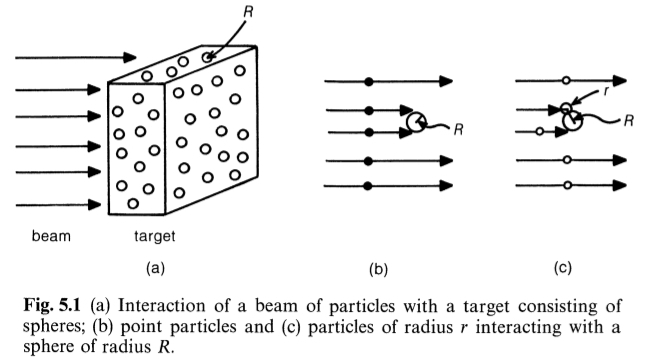
\includegraphics[width=4.5in]{immagini/cross-section.jpg} %immagine
\end{center}

Tuttavia, la probabilità di una reazione che si svolge può ancora essere misurata in termini di una sezione trasversale d'urto che continueremo ad indicare con $\sigma$. $\sigma$ può fare riferimento alla \textbf{sezione totale d'urto} (indicato con $\sigma_T$), che riguarda la probabilità che accada qualcosa quando particella e bersaglio interagiscono o può essere una \textbf{sezione trasversale parziale} $\sigma_i$ che riguarda la probabilità che una reazione specifica (indicata con i) avrà luogo. Chiaramente
\begin{equation}
\sigma_T=\sum_i{\sigma_i}.
\end{equation}

Sebbene $\sigma$ non sia la sezione geometrica di un nucleo, anche se ciò potrebbe essere definito con precisione, e può essere più grande o più piccolo di questo, è tuttavia prevedibile che sarà di questo ordine di grandezza. Poiché i nuclei hanno raggi $R$ nella regione da 2 fm a 7 fm, in modo che $\pi R^2$ sia nella regione da $5 \cdot 10^{-29}$ \si{m^2} a $1.5 \cdot 10^{-27}$ \si{m^2}, \textbf{si è soliti esprimere le sezioni d'urto delle reazioni nucleari in barn}.

\begin{center}
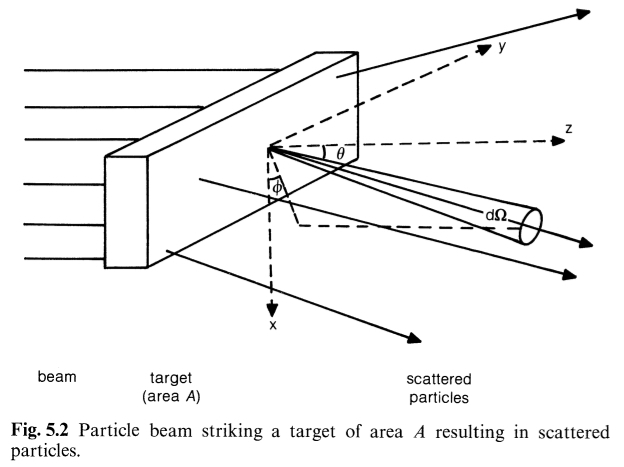
\includegraphics[width=4.5in]{immagini/cross-section-2.jpg} %immagine
\end{center}

Infine si introduce il concetto di \textbf{sezione d'urto differenziale} che è indicata con $$\frac{\textrm{d}\sigma}{\textrm{d}Q}.$$ Viene utilizzato quando la distribuzione angolare dei prodotti di un'interazione nucleare è sotto esame. La situazione è illustrata nella figura in cui i prodotti di reazione sono mostrati in movimento in una direzione specificata come al solito dagli angoli solidi polari $\theta$ e $\phi$ nell'angolo solido $\textrm{d}\Omega=\sin\left(\theta\right)\textrm{d}\theta\textrm{d}\phi$.

Per una data reazione nucleare, mentre \textbf{$\sigma$ si riferisce alla probabilità che avvenga la reazione}, \textbf{$\frac{\textrm{d}\sigma}{\textrm{d}Q}$ riguarda la probabilità che i prodotti di reazione siano trovati in movimento nella direzione ($\theta$, $\phi$)}. $\frac{\textrm{d}\sigma}{\textrm{d}Q}$ sarà in generale una funzione di $\theta$ e $\phi$, sebbene la direzione di incidenza, siccome le particelle, bombardando nuclei bersaglio, hanno i loro spin orientati in modo casuale, sarà un asse di simmetria e $\frac{\textrm{d}\sigma}{\textrm{d}Q}$ sarà indipendente da $\phi$.

\textbf{Se la sezione d'urto differenziale è integrata nel angolo solido $4\pi R$ si ottiene la sezione d'urto}: perciò
\begin{equation}
\sigma=\int^{4\pi}{\frac{\textrm{d}\sigma}{\textrm{d}Q}\textrm{d}\Omega}.
\end{equation}

\section{Processi di reazione nucleare} %Processi di reazione nucleare
La particella incidente si scontra con un nucleone nel nucleo bersaglio, forse uno che giace in un livello molto basso nel modello a shell, e nessuno dei due ha energia sufficiente per fuggire. Ci sarà poi una serie di ulteriori collisioni casuali nel nucleo finché alla fine abbastanza energia è concentrata per caso su una particella per consentirle di fuggire; o il nucleo può perdere la sua energia emettendo radiazione elettromagnetica. Questo stato di nucleo, dopo aver catturato la particella incidente e in cui molti processi di collisione interne si verificano, è stato discusso da Niels Bohr nel 1936 ed è indicato come il \textbf{nucleo composto}.

Considerando che una reazione diretta, per una particella incidente di vari \si{MeV}, avviene in un tempo dell'ordine di quanto impiega un nucleone per attraversare un nucleo (quindi circa $\si{10^{-22}}{s}$), \textbf{esiste il nucleo composto per un periodo molto più lungo e che può esistere per tempi nella regione approssimativa da $\si{10^{-14}}{s}$ a $\si{10^{-20}}{s}$}.

\textbf{In certe regioni di energia la sezione d'urto ha dei picchi che corrispondono a degli stati risonanti}. Aumentando l'energia i picchi si allargano fino a non poter più distinguere gli stati risonanti: ci sono sovrapposizioni.

Un modello che dà una descrizione unificata è il \textbf{modello ottico}, che descrive lo scattering elastico come dovuto ad un potenziale complesso di cui la \textbf{parte reale} è del tipo del modello a shell mentre la \textbf{parte immaginaria} tiene conto dei cambi diversi di reazione, se essi sono possibili, che assorbono parte del flusso incidente. \textbf{Si chiama ottico in analogia con l'indice di rifrazione complesso}. \textbf{Il nucleo è visto come una palla di cristallo opaca}. Si sono trascurate le reazioni che coinvolgono particelle non nucleari o ioni pesanti.

\section{Reazioni dirette} %Reazioni dirette

Le reazioni dirette più comunemente si verificano durante il breve periodo di contatto tra le particelle che si scontrano in una collisione periferica. I più semplici sono quelli che procedono attraverso un processo a singola fase, come l'eccitazione di un nucleone in scattering anelastico da uno stato del modello a shell in un nucleo ad un altro. \textbf{Le reazioni dirette sono caratterizzate da una singola collisione di una particella incidente con un nucleone nel nucleo}. Questa collisione avviene normalmente nella regione della superficie nucleare dal momento che una penetrazione più profonda rischia di portare a collisioni multiple e la formazione di un nucleo composto.

\textbf{Il nucleone può essere eccitato (scattering anelastico), o prelevato [ad esempio in una reazione (p,d)], o un nucleone da una particella composta incidente può essere catturato in uno stato di energia nucleare [ad esempio in una reazione (d,n)]}. In qualsiasi forma, la reazione porta generalmente alla popolazione di un basso stato eccitato del nucleo. In queste reazioni, se lo stato finale è fortemente popolato, è collegato in modo semplice allo stato iniziale dal meccanismo di reazione. È per questo motivo che diverse reazioni dirette sono utilizzati per eccitare e identificare stati nucleari che hanno strutture e proprietà differenti.

\textbf{Coinvolgendo solo una collisione, tali reazioni sono abbastanza facili da capire e interpretare e sono particolarmente utili per le descrizioni test del modello shell di stati nucleari}.

\chapter{Fissione} %Fissione
Si immagini un \textbf{neutrone che va a colpire un nucleo}. Il neutrone è di bassa energia. Si è in una regione in cui si forma un sistema composto. Il nucleo potrebbe assorbire il neutrone formando un isotopo artificiale con un'emissione radioattiva $\gamma$ con $Q\simeq \si{4-10}$ \si{MeV}: $$n+\ce{^A_ZX}\longrightarrow \ce{^{A+1}_ZX}+\gamma.$$ Sebbene \ce{^A_ZX} sia stabile, può accadere che \ce{^{A+1}_ZX} non lo sia più. Può essere che diventi più stabile se un neutrone diventa un protone, quindi se avviene un decadimento $\beta$: $$\ce{^{A+1}_ZX}\longrightarrow \ce{^{A+1}_{Z+1}X}+e^-+\bar\nu_e+Q.$$ È l'esempio di $n+\ce{^{115}_{49}In} \longrightarrow \ce{^{116}_{49}In}\longrightarrow \ce{^{116}_{50}Sn}+e^-+\bar\nu_e$.

Partendo da queste idee, Fermi pensava di far assorbire un neutrone all'uranio per produrre artificialmente elementi transuranici. In realtà con questo processo con neutroni lenti su uranio si è vista la fissione. Sugli elementi prodotti si sono fatti test chimici: si è ottenuto $Z$ tra 50 e 60, non oltre il 92 dell'uranio come ci si aspettava. L'uranio infatti si divide dopo la cattura del neutrone. \textbf{Da un nucleo pesante si formano due nuclei più leggeri, una produzione di altri neutroni e di energia}.

L'energia di legame per nucleone è, in modulo, più alta per $Z$ più vicino a 50 che a 90: \textbf{nel processo si libera energia}. Ci sono circa 0.9 MeV per nucleone di differenza che portano a $\simeq$\si{200}{ MeV} in totale per ogni atomo che si scinde in due.

Si fa riferimento al \textbf{modello a goccia di liquido}.

\textbf{Nel nucleo ci sono due forze che competono: l'interazione coulombiana e l'interazione nucleare}.

Per i nuclei con $Z$ grande aumenta la repulsione coulombiana e servono quindi più neutroni per la stabilità: \ce{^{240}_{146}Pu} $\frac{N}{A}\simeq 0.61$ MeV, \ce{^{120}_{50}Sn} $\frac{N}{A}\simeq 0.59$ MeV.

L'interazione nucleare è simile alla forza di coesione di un liquido. \textbf{La forma più stabile per l'interazione nucleare è quella sferica, ma è la più instabile per la repulsione coulombiana perché la distanza tra le parti è minima}.

Nel modello a goccia di liquido \textbf{guardiamo solo il termine di superficie e il termine coulombiano} (il volume totale si conserva):
\begin{equation}\begin{split}
V_{S} \propto A^{\frac{2}{3}} \sim Z^{\frac{2}{3}} \\
V_{C}\propto Z^2.
\end{split}\end{equation}
Aumentando $Z$ prevale $V_C$, che tende a rompere il nucleo.

\begin{center}
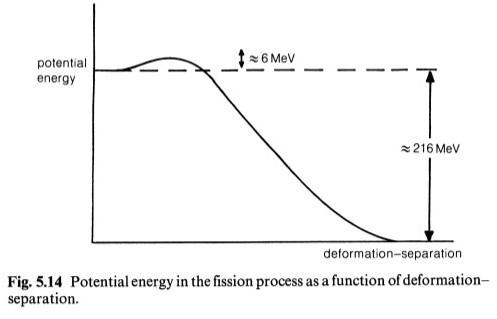
\includegraphics[width=4in]{immagini/pot_fission.jpg} %immagine
\end{center}

Se il nucleo oscilla attorno alla forma sferica, deformandosi, e se le oscillazioni sono grandi anch'esse (alta energia di eccitazione), \textbf{la deformazione può essere così grande che le due parti si separino}:

\begin{center}
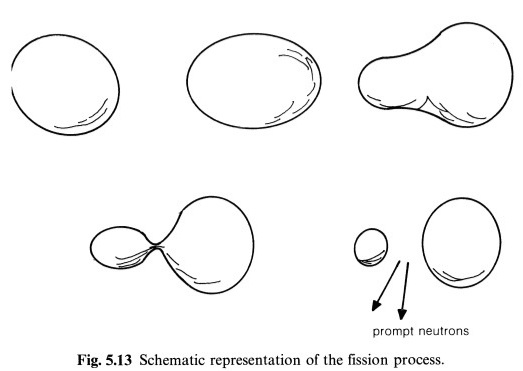
\includegraphics[width=4.5in]{immagini/fission.jpg} %immagine
\end{center}

\section{Fissione spontanea} %Fissione spontanea
Essendo il nucleo iniziale di forma sferica e il nucleo deformato di forma ellissoidale e dovendosi conservare il volume si ha:
\begin{equation*}\begin{split}
a=R\left(1+\epsilon\right)\\
b=R\left(1+\epsilon\right)^{\frac{1}{2}}
\end{split}\end{equation*}
essendo $ab^2=R^2$ ed $\epsilon$ la piccola oscillazione. \textbf{La superficie aumenta} rispetto a quella sferica: $S=\frac{4}{3}\pi R^2\left(1+\frac{2\epsilon^2}{5}+\dots\right)$. \textbf{Aumenta} anche \textbf{la distanza media}: $\left\langle \frac{1}{r} \right\rangle=\frac{3}{5R}\left(1-\frac{\epsilon^2}{5}\right)$.

Tra la forma sferica e quella deformata si ha:
\begin{equation}\begin{split}
\Delta M=\\
=a_SA^{\frac{2}{3}}\left(-\frac{2\epsilon^2}{5}\right)+a_C\frac{Z^2}{A^{\frac{1}{3}}}\left(\frac{\epsilon^2}{5}\right)=\\
=\frac{\epsilon^2}{5}A^{\frac{2}{3}}\left(-2a_S+a_C\frac{Z^2}{A}\right)
\end{split}\end{equation}
La condizione di stabilità è che $\Delta M<0$ altrimenti il nucleo si rompe.

Inserendo i valori di $a_S=17$ e di $a_C=0.7$ si ottiene che per avere $\Delta M<0$ si deve avere
\begin{equation}\begin{split}
\frac{Z^2}{A}\ge 47.
\end{split}\end{equation}
Per i nuclei stabili questo rapporto vale circa 35, e questo dimostra che \textbf{la fissione spontanea è poco probabile}. Ovviamente tutto questo è nell'ipotesi di piccole deformazioni. \textbf{L'aumento di energia si oppone alla deformazione. I neutroni possono} però \textbf{fornire l'energia di attivazione necessaria}.

Se $A\le 250$, per esempio l'uranio, il tempo di vita per fissione spontanea è $10^{16}$ anni. È più probabile che abbia un decadimento $\alpha$ ($\tau\sim 10^9$ anni).

\textbf{Per A maggiori di 250 si ha} invece \textbf{una certa probabilità di fissione spontanea} (per il \si{Fm} il tempo è 157 minuti). Il decadimento $\alpha$ è invece meno probabile.

\subsection{Modello di Bohr e Wheeler} %Modello di Bohr e Wheeler
Si ha $$\ce{^{A}_ZX}\longrightarrow\ce{^{A/2}_{Z/2}Y}+\ce{^{A/2}_{Z/2}Y}.$$ In realtà nella fissione non c'è divisione esatta in due nuclei uguali. Si ottiene quindi:
\begin{equation}\begin{split}
Q=\\
=a_S\left[A^{\frac{2}{3}}-2\left(\frac{A}{2}\right)^{\frac{2}{3}}\right]+a_C\left[\frac{Z^2}{A^{\frac{1}{3}}}-2\frac{\left(\frac{Z}{2}\right)^2}{\left(\frac{A}{2}\right)^{\frac{1}{3}}}\right]=\\
=A^{\frac{2}{3}}\left[a_S\left(1-2^{\frac{1}{3}}\right)+a_C\frac{Z^2}{A}\left(1-2^{\frac{2}{3}}\right)\right]\simeq\\
\simeq A^{\frac{2}{3}}\left(-4.4+0.26\frac{Z^2}{A}\right).
\end{split}\end{equation}
Deve essere $Q\ge 0$ perché il processo avvenga, perciò si deve avere $\frac{Z^2}{A}\ge 17$.

I due nuclei $Y$ restano comunque legati dal potenziale nucleare, cioè \textbf{non si ha fissione, se non si allontanano più della distanza somma dei raggi dei due nuclei} (che va come $2R_0\left(\frac{A}{2}\right)^{\frac{1}{3}}$). C'è una barriera di energia di $E_b\simeq$200 MeV.

\begin{itemize}
\item Se $\frac{Z^2}{A}\ge 47$ si ha $E_b-Q>0$: \textbf{fissione spontanea}, ma con $A\sim 300$ che \textbf{non esistono}.
\item Se $\frac{Z^2}{A}\simeq 17$ si ha $E_b-Q\simeq 60$ MeV: \textbf{non c'è fissione}, con $A\simeq 100$.
\item \textbf{Se $A\simeq 240$ (uranio, plutonio...) si ha $E_b-Q\simeq 6$ MeV: la barriera di energia può essere superata con una certa probabilità per effetto tunnel oppure con fissione indotta (inviando neutroni)}.
\end{itemize}

Per fare il conto per bene, comunque, bisogna includere anche gli altri termini del modello a goccia di liquido.

\section{Fissione dell'uranio} %Fissione dell'uranio
Considerando l'uranio naturale, mescolanza di due isotopi: $$99.3\%\ce{^{238}_{92}U}+0.7\%\ce{^{235}_{92}U}$$ si ha per l'isotopo più presente
\begin{equation}\begin{split}
n+\ce{^{238}_{92}U}\longrightarrow \ce{^{239}_{92}U}^*
\end{split}\end{equation}
con $n$ un neutrone lento di energia piccola ($\simeq 0$), chiamato \textbf{neutrone termico}, e $U^*$ uno stato eccitato con energia di attivazione $\simeq 5$ MeV, cioè circa 1 MeV più basso di quanto si usi per superare la barriera. Si ha altrimenti, per l'altro isotopo
\begin{equation}\begin{split}
n+\ce{^{235}_{92}U}\longrightarrow \ce{^{236}_{92}U}^*
\end{split}\end{equation}
con un'energia di eccitazione di 6.4 MeV sufficiente a innescare la fissione. In questo caso \textbf{l'energia è più alta perché l'atomo è pari-pari, quindi più stabile}.

In generale i frammenti che derivano dalla fissione non sono uguali (ad esempio per l'uranio 238 i picchi sono sottoprodotti con $A\simeq 95$ e $A\simeq 140$). La distribuzione delle masse dei frammenti è, in scala logaritmica, del tipo

\begin{center}
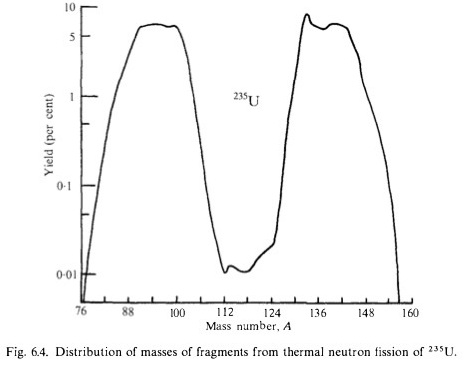
\includegraphics[width=4.3in]{immagini/mass_fission.jpg} %immagine
\end{center}

\subsection{Caso dell'uranio} %Caso dell'uranio
\begin{equation}\begin{split}
n+\ce{^{235}_{92}U}\longrightarrow \ce{^{87}_{35}Br}+\ce{^{148}_{57}La}+n \\
n+\ce{^{235}_{92}U}\longrightarrow \ce{^{93}_{37}Rb}+\ce{^{141}_{55}Cs}+2n \\
n+\ce{^{235}_{92}U}\longrightarrow \ce{^{140}_{56}Ba}+\ce{^{93}_{36}Kr}+3n
\end{split}\end{equation}
A loro volta i frammenti possono decadere in vari modi. Ad esempio dopo 5 decadimenti $\beta^-$ con tempo $\tau_{\frac{1}{2}}$ di 2 secondi o $10^6$ anni. Da \ce{^{93}_{36}Kr} si arriva a \ce{^{93}_{41}Nb}, da \ce{^{140}_{56}Ba} in 128 giorni con un decadimento $\beta^-$ si arriva a \ce{^{140}_{57}La} che con decadimento $\beta^-$ da \ce{^{140}_{58}Ce}... Queste sono le \textbf{scorie radioattive, le quali hanno vita media lunga}. $$\ce{^{93}Rb}\longrightarrow_{\textrm{in 6 s}} \ce{^{93}Sr}\longrightarrow_{\textrm{in 420 s}} \ce{^{93}Y} \longrightarrow_{\textrm{in 10 h}} \ce{^{93}Zr}\longrightarrow_{\textrm{in }10^{6}\textrm{ anni}} \ce{^{93}Nb}.$$ L'energia liberata dalla fissione viene raccolta dai frammenti, in energia cinetica dei neutroni, in energia emessa da ulteriori decadimenti, ...

\section{Reazioni a catena} %Reazioni a catena
I neutroni liberati (\textbf{neutroni veloci o prompt}) dalla reazione possono essere usati per innescare una reazione a catena. Alcuni saranno dispersi, altri andranno a stimolare altre fissioni. Ci possono essere tre situazioni:
\begin{itemize}
\item \textbf{Critica}: almeno 1 neutrone innesca un'altra fissione;
\item \textbf{Supercritica}: più di 1 neutrone innesca un'altra fissione (rischio di esplosione);
\item \textbf{Sottocritica}: meno di 1 neutrone innesca un'altra fissione.
\end{itemize}

I \textbf{parametri che servono per analizzare e controllare la reazione} sono:
\begin{itemize}
\item il numero $\nu$ di neutroni emessi per fissione;
\item la distribuzione in energia dei neutroni emessi;
\item la probabilità $\rho$ di indurre un'altra fissione.
\end{itemize}
Da una fissione originaria possono avvenire $\rho\nu$ fissioni secondarie e $\left(\rho\nu\right)^2$ reazioni terziarie. 

$\rho$ dipende da molti fattori: sezione d'urto, forma geometrica del materiale ed è inversamente proporzionale alla superficie. \textbf{È meglio minimizzare la superficie}: \textbf{si ricorre alla forma sferica}. Se cresce il raggio cala ancora il rapporto superficie/volume. Si arriva a un \textbf{raggio critico} a cui corrisponde una \textbf{massa critica} per la quale la produzione di neutroni e la probabilità di fuga si compensano. In queste condizioni $\rho\nu=1$.

Si può usare un \textbf{moderatore} che rallenti ma non catturi i neutroni, ad esempio il carbonio o l'acqua pesante. Per diminuire $\rho$ si può invece usare qualche materiale che catturi i neutroni, come ad esempio delle barre di controllo in cadmio.

\subsection{Armi nucleari} %Armi nucleari
\textbf{Due masse sottocritiche rapidamente unite a formare massa supercritica}. Nelle bombe atomiche si arricchisce anche fino al 90\%.

\subsection{Reattori termici} %Reattori termici
\textbf{Si usa l'uranio 235 presente in natura, eventualmente arricchendo la miscela naturale, che fissiona con neutroni lenti (termici)}. Si usa un moderatore per rallentare i neutroni emessi dalle fissioni che sono a circa 1 MeV. Per controllare il tasso delle reazioni si usano barre di controllo con sezioni d'urto molto alte per la cattura di neutroni termici. I neutroni di fissione, tuttavia, hanno energie intorno a 1 MeV e così devono essere rallentati rapidamente alle energie termiche basse necessarie. L'energia è più efficacemente persa dallo scattering di un corpo (noto come moderatore) avente una massa simile a quella di un neutrone, ad esempio idrogeno, deuterio, ecc.

Per arricchire la miscela di uranio naturale si ha $$n+\ce{^{238}_{92}U}\longrightarrow_{\gamma} \ce{^{239}_{92}U}\longrightarrow_{\beta} \ce{^{239}_{93}Np}\longrightarrow_{\beta} \ce{^{239}_{94}Pu} \quad \textrm{ fissile con neutroni termici}.$$ Un ciclo acqua-vapore assorbe il calore prodotto e aziona una turbina per la produzione di energia elettrica.

\subsection{Reattori veloci} %Reattori veloci
\textbf{Si usano neutroni energetici per sfruttare anche \ce{^{238}U}}. \textbf{Non serve un moderatore}. Si produce molto più calore e perciò si raffredda a sodio liquido. Il neutrone in \ce{^{239}Pu} permette ad esso di decadere anche con neutroni veloci e perciò \textbf{il reattore si può autoalimentare}. Il reattore si autosostiene se $\rho\nu=1$. Un ciclo acqua-vapore assorbe il calore prodotto e aziona una turbina per la produzione di energia elettrica.

Un reattore termico non funzionerà in questo modo perché ad energie termiche troppi neutroni vengono assorbiti dal \ce{^{239}Pu} attraverso la cattura radiativa.

\chapter{Fusione} %Fusione
\begin{center}
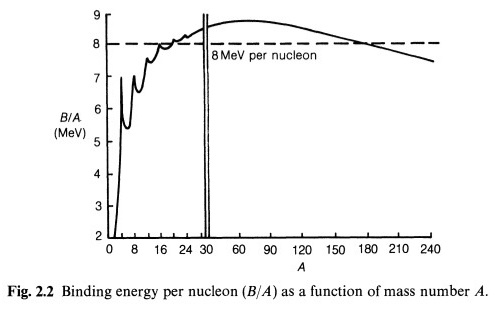
\includegraphics[width=4.5in]{immagini/bound_energy.jpg} %immagine
\end{center}

\textbf{Nuclei leggeri si uniscono a formarne uno pesante}. $$\ce{^{A_1}_{Z_1}X}+\ce{^{A_2}_{Z_2}}Y\longrightarrow \ce{^{A_1+A_2}_{Z_1+Z_2}W}+Q.$$

\textbf{I due nuclei devono avvicinarsi tanto da risentire dell'attrazione nucleare: devono avere energia sufficiente a superare la repulsione coulombiana ed entrare nel campo d'azione dell'interazione nucleare}. $$\ce{^{12}_6C}+\ce{^{12}_6C}\longrightarrow \ce{^{24}_{12}Mg}+ 13.9 \textrm{ MeV}.$$ I due atomi di carbonio devono avere energia cinetica totale $\ge 9$ MeV. Il guadagno è quindi di $13.9-9=4.9$ MeV. \textbf{L'energia emessa diventa energia cinetica dei nuclei prodotti}.

Se sono confinati da un campo di forza (si raggiunge la condizione di equilibrio nel quale il processo si autosostiene), aumenta la temperatura e perciò avviene una produzione di calore.

\section{Fusione in laboratorio} %Fusione in laboratorio
Ci sono tre stati nel ciclo dell'idrogeno che si riesce a compiere in un laboratorio (con \ce{D} si intende il deuterio):
\begin{equation}\begin{split}
p+p\longrightarrow \ce{D}+e^-+\nu_e \qquad 0.42 \textrm{ MeV} \\
p+\ce{D}\longrightarrow \ce{^3_2He}+\gamma \qquad 5.49 \textrm{ MeV} \\
\ce{^3_2He}+\ce{^3_2He}\longrightarrow \ce{^4_2He}+2p \qquad 12.86 \textrm{ MeV}
\end{split}\end{equation}
Complessivamente entrano 4 protoni e risultano 2 positroni, 2 neutrini e un atomo di elio:
\begin{equation}\begin{split}
4p\longrightarrow \ce{^4_2He} +2\gamma+2e^-+2\nu_e
\end{split}\end{equation}
\begin{equation}\begin{split}
Q=\left[4m_p-M\left(\ce{^4_2He}\right)-2m_e\right]c^2=24.7 \textrm{ MeV}
\end{split}\end{equation}
Per tenere conto dell'energia emessa, di quella dei neutroni e di un'ulteriore annichilazione dei positroni si ha un bilancio di $\sim 26$ MeV.

\section{Fusione nelle stelle} %Fusione nelle stelle
\subsection{Sole} %Sole
\textbf{Temperatura}: $1.5\cdot 10^{7}$ K. \textbf{Energia cinetica}: $\frac{3}{2}K_bT\sim 10^3$ eV.

L'energia cinetica data dalla temperatura dei plasmi stellari è sufficiente ad instaurare la reazione tra nuclei di idrogeno (protoni) per formare elio (in realtà quest'energia è al di sotto della barriera coulombiana: la reazione procede grazie ad effetti quantistici come l'effetto tunnel, ma a ritmi piuttosto bassi).

\subsection{Altri cicli} %Altri cicli
$$\ce{^4_2He}+\ce{^4_2He}\longrightarrow \ce{^8_4Be}$$ $$\ce{^4_2He}+\ce{^8_4Be}\longrightarrow \ce{^{12}_6C}^*.$$ Esaurito il ciclo dell'idrogeno per le stelle, il carbonio cristallizza in un altro ciclo con risultato netto
\begin{equation}\begin{split}
4p\longrightarrow \ce{^4_2He}+2e^-+3\gamma+2\nu_e \qquad Q=26.1\textrm{ MeV}
\end{split}\end{equation}
Avvengono in genere a temperature più alte dei precedenti cicli e si ottiene il \textbf{ciclo del carbonio}. I processi del ciclo sono:
\begin{equation}\begin{split}
\ce{^{12}C}+p\longrightarrow \ce{^{13}N}+\gamma \qquad 1.94\textrm{ MeV} \\
\ce{^{13}N}\longrightarrow_{\beta^+} \ce{^{13}C}+e^++\nu \qquad 1.20\textrm{ MeV} \\
\ce{^{13}C}+p\longrightarrow \ce{^{14}N}+\gamma \qquad 7.55\textrm{ MeV} \\
\ce{^{14}N}+p\longrightarrow \ce{^{15}O}+\gamma \qquad 7.29\textrm{ MeV} \\
\ce{^{15}O}\longrightarrow_{\beta^+} \ce{^{15}N}+e^++\nu \qquad 1.73\textrm{ MeV} \\
\ce{^{15}N}+p\longrightarrow \ce{^{12}C}+\ce{^4He} \qquad 4.96\textrm{ MeV}
\end{split}\end{equation}

La somma dei $Q$ con l'energia data dall'annichilazione dei positroni dà la $Q$ totale pari a 26.7 MeV.

\paragraph{Sintesi di nuclei più pesanti}
\begin{itemize}
\item $\ce{^{4}_{2}He}+\ce{^{17}_{6}C}\longrightarrow \ce{^{16}_{8}O}+\gamma$: $Q=7.16$ MeV (l'energia coulombiana richiesta per innescare il processo è 3.6 MeV)
\item $\ce{^{4}_{2}He}+\ce{^{16}_{8}O}\longrightarrow \ce{^{20}_{10}Ne}+\gamma$: $Q=4.73$ MeV (l'energia coulombiana richiesta per innescare il processo è 4.5 MeV)
\item $\ce{^{4}_{2}He}+\ce{^{20}_{10}Ne}\longrightarrow \ce{^{24}_{12}Mg}+\gamma$: $Q=9.31$ MeV (l'energia coulombiana richiesta per innescare il processo è 3.4 MeV)
\end{itemize}
\textbf{Se la stella ha concluso \ce{He} si contrae, aumenta la temperatura e può bruciare i nuclei più pesanti, almeno fino ai nuclei per cui la fusione è esotermica}. I nuclei pesanti sono meno abbondanti nell'universo perché più difficili da produrre. Sono più spesso formati per aggiunta di neutroni che attraverso la fusione.

I nuclei oltre il ferro non sono più sintetizzati per fusione ma con reazioni tipo:
\begin{equation}\begin{split}
n+\ce{^A_ZX}\longrightarrow \ce{^{A+1}_ZX}^*\longrightarrow_{\gamma} \ce{^{A+1}_ZX}+\gamma\\
\ce{^{A+1}_ZX}\longrightarrow_{\beta^-} \ce{^{A+1}_{Z+1}Y}+e^-+\bar\nu_e.
\end{split}\end{equation}
\textbf{L'abbondanza relativa dei nuclei pesanti dipende dalle probabilità di cattura neutronica ($n\longrightarrow p+e^-+\bar\nu_e$) e di decadimento $\beta$}.

Idrogeno ed elio si crearono nella nucleosintesi primordiale e sono i più abbondanti elementi nell'universo. L'elio è una particella $\alpha$ e gioca un ruolo importante nella nucleosintesi stellare: \textbf{sono abbondanti gli elementi che sono insiemi di particelle $\alpha$}. \textbf{Sono abbondanti nell'universo anche i nuclei con numeri magici}.

\textbf{La fusione è più vantaggiosa della fissione: energeticamente i risultati sono migliori per la fusione, il ``carburante'' è più abbondante e non ci sono sottoprodotti dannosi o scorie}. I maggiori problemi sono di natura tecnica: le altissime temperature necessarie a dar sufficiente energia per innescare la fusione. \textbf{La materia è allo stato di plasma}. Gli $e^-$ sottraggono al sistema energia emettendo radiazioni.

Tra le reazioni più promettenti si ha:
\begin{equation*}\begin{split}
\ce{^2_1H}+\ce{^3_1He}\longrightarrow \ce{^4_2He}+n
\end{split}\end{equation*}
con $Q=17.6$ MeV. Essa avviene a temperature non troppo elevate, rispetto alla fusione solita, e con densità non troppo alte. Il rendimento energetico è buono. Il problema sta nel confinare il plasma: si pensa a confinamento magnetico o inerziale.

\chapter{Radioattività} %Radioattività
La dipendenza temporale è data dalla legge del decadimento radioattivo. \textbf{Il decadimento è un processo statistico, possiamo dare solo una probabilità che un nucleo decada ad un certo istante}. La \textbf{probabilità di decadimento} in $\Delta t$ è proporzionale al tempo:
\begin{equation}\begin{split}
\textrm{d}p=\lambda \textrm{d}t
\end{split}\end{equation}
con $\lambda$ costante di decadimento.

Considerando una sostanza con $N$ nuclei, la probabilità di decadere di un singolo nucleone non dipende da $N$. Nel tempo $\textrm{d}t$ ci saranno $$N\textrm{d}p=N\lambda \textrm{d}t$$ decadimenti. La variazione nei nuclei sarà $$-\textrm{d}N=N\lambda \textrm{d}t$$ da cui si ricava la \textbf{legge di decadimento esponenziale}:
\begin{equation}\begin{split}
N\left(t\right)=N\left(0\right)e^{-\lambda t}
\end{split}\end{equation}

Si può parlare di \textbf{attività} di una sostanza radioattiva; essa è definita come \textbf{numero di decadimenti nell'unità di tempo}:
\begin{equation}\begin{split}
A\left(t\right)=\left|\frac{\textrm{d}N}{\textrm{d}t}\right|=\lambda N\left(t\right)=\lambda N\left(0\right)e^{-\lambda t}
\end{split}\end{equation}
(si noti che anch'essa decresce in modo esponenziale).

La componente attiva, ad esempio del torio \ce{Th}, viene detta, dai primi sperimentatori, \ce{ThX} (o uranio X per l'uranio), in cui il \ce{Th} decade per processo $\alpha$. Quello che succede veramente è che il \ce{ThX} è radio \ce{Ra}:
\begin{equation}\begin{split}
\ce{^{232}_{90}Th}\longrightarrow_{\alpha} \ce{^{228}_{88}Ra}
\end{split}\end{equation}
e il radio decade radioattivamente. Il \ce{Ra} decade esponenzialmente ma si riforma perché il \ce{Th} originario continua a decadere.

L'idea è quella delle \textbf{catene radioattive}.

\paragraph{Unità di misura} L'unità adottata nel S.I. è il Becquerel: 1 Bq equivale ad una disintegrazione per secondo. Un suo multiplo è il Curie: 1 Ci=$3.7\cdot 10^{10}$ Bq. Essa è l'attività di 1 g di radio.

\paragraph{Tempo di vita medio} 
\begin{equation}\begin{split}
|\textrm{d}N|=\lambda N\left(0\right)e^{-\lambda t}\textrm{d}t\\
\Longrightarrow \tau=\frac{1}{N\left(0\right)}\int_{N\left(0\right)}^0{t|\textrm{d}N|}=\frac{\int{t\textrm{d}N}}{\int{\textrm{d}N}}=\frac{1}{\lambda}\\
\Longrightarrow N\left(t\right)=N\left(0\right)e^{-\frac{1}{\tau}}.
\end{split}\end{equation}
Per misurare $\tau$ si pone in un grafico $\ln{\left[A\left(t\right)\right]}=\ln{\left[\lambda N\left(0\right)\right]}-\lambda t$: la pendenza del grafico fornisce $\lambda$. Va bene per $\tau$ non troppo piccoli.

\paragraph{Tempo di dimezzamento} Tempo nel quale decadono la metà dei nuclei:
\begin{equation}\begin{split}
\frac{N\left(0\right)}{2}=N\left(0\right)e^{-\frac{t_{1/2}}{\tau}}\\
\Longrightarrow t_{\frac{1}{2}}=\ln{\left(2\right)}\tau=\frac{\ln{\left(2\right)}}{\lambda}.
\end{split}\end{equation}

\paragraph{Ampiezza in energia di uno stato nucleare}
\begin{equation}\begin{split}
\Gamma=\Delta E \sim \frac{\hbar }{\tau}.
\end{split}\end{equation}
Più $\tau$ è lungo, più l'energia dello stato è definita.

\section{Processi a catena} %Processi a catena
$$1\longrightarrow 2$$
\begin{equation}\begin{split}
\textrm{d}N_1=-\lambda_1N_1 dt\\
\textrm{d}N_2=-\lambda_2N_2 dt+\lambda_1N_1 dt
\end{split}\end{equation}
\begin{equation}\begin{split}
N_1\left(t\right)=N\left(0\right)e^{-\lambda_1 t}\\
N_2\left(t\right)=ae^{-\lambda_1t}+be^{-\lambda_2t}
\end{split}\end{equation}

A $t=0$ si ha:
\begin{equation}\begin{split}
N_1\left(0\right)=N_0\\
N_2\left(0\right)=a+b=0\\
\Longrightarrow a=-b=\frac{N_0\lambda_1}{\lambda_2-\lambda_1}\\
\Longleftrightarrow \left.\frac{\textrm{d}N_2}{\textrm{d}t}\right|_{t=0}=-a\lambda_1-b\lambda_2=\lambda_1N_0
\end{split}\end{equation}

Si ottengono quindi le ampiezze:
\begin{equation}\begin{split}
A_1\left(t\right)=N_0\lambda_1e^{-\lambda_1t}\\
A_2\left(t\right)=\frac{N_0\lambda_1}{\lambda_2-\lambda_1}\left(e^{-\lambda_1t}e^{-\lambda_2t}\right)
\end{split}\end{equation}

La situazione può anche essere più complessa $$1\longrightarrow 2\longrightarrow 3\dots$$

\chapter{Decadimenti} %Decadimenti
\textbf{In natura molti elementi radioattivi sono generati da nuclei capostipite}. Ci sono 4 catene (o famiglie) radioattive in natura, cioè insiemi di nuclei che derivano dallo stesso capostipite. \textbf{L'unico decadimento che cambia il numero di nucleoni è quello $\alpha$}, infatti decadimento $\beta$ non cambia il numero di nucleoni. Si hanno salti di 4 unità:
\begin{equation}\begin{split}
\frac{A-x}{4}=n.
\end{split}\end{equation}
\textbf{Da ogni capostipite si parte sempre con un decadimento $\alpha$}. Ogni 4 nucleoni si ricade infatti nella stessa famiglia (c'è una particella $\alpha$ in più o in meno) e ne è un esempio il torio \ce{Th}.

\paragraph{Tempo di vita della Terra} Il fatto che esistano queste famiglie ci dà un'idea del tempo di vita della Terra. In realtà la catena del nettunio \ce{^{237}Np} non esiste più in natura, ma solo artificialmente; ciò significa che l'età della Terra è indicativamente più grande del tempo di dimezzamento del \ce{^{237}Np}, cioè $10^6$ anni.

Una \textbf{stima più precisa dell'età della terra} può essere fatta in modo più rigoroso: immaginando originariamente le stesse percentuali di \ce{^{238}U} e \ce{^{235}U}, si confronta con la situazione odierna, cioè 140 atomi di 238 per ogni atomo di 235. $$N_1\left(t\right)=\frac{N_2\left(t\right)}{140} \Longrightarrow t=\frac{\tau_1\tau_2}{\tau_2-\tau_1}\ln{\left(140\right)}\simeq 10^{10} \textrm{ anni}$$ avendo considerato $\tau_i=\frac{\left(\tau_i\right)_{1/2}}{\ln{\left(2\right)}}$.

\section{Alpha $\alpha$} %α
\begin{equation}\begin{split}
M\left(A,Z\right)\longrightarrow M\left(4,2\right)+M\left(A-4,Z-2\right)\\
Q=\left[M\left(A,Z\right)-M\left(4,2\right)-M\left(A-4,Z-2\right)\right]c^2
\end{split}\end{equation}
La \textbf{reazione avviene se $Q>0$}.

\textbf{L'energia emessa da un decadimento $\alpha$ va a finire quasi tutta in energia cinetica della particella $\alpha$}.
\begin{equation}\begin{split}
Q=T_d+T_{\alpha}
\end{split}\end{equation}
con $T_d=\frac{1}{2}m_dv^2_d$ si intende la particella figlia. Per la conservazione del momento si ha inoltre $m_dv_d=m_{\alpha}v_{\alpha}$:
\begin{equation}\begin{split}
v_d=\frac{m_{\alpha}}{m_d}v_{\alpha}.
\end{split}\end{equation}
\textbf{Considerando che $m_{\alpha}\ll m_d$ si ha $v_d\ll v_{\alpha}$}.
\begin{equation}\begin{split}
Q=\frac{1}{2}m_d\left(\frac{m_{\alpha}}{m_d}v_{\alpha}\right)^2+\frac{1}{2}m_{\alpha}v^2_{\alpha}=\frac{1}{2}m_{\alpha}v_{\alpha}\left(1+\frac{m_{\alpha}}{m_d}\right)\\
\Longrightarrow T_{\alpha}=Q\frac{m_d}{m_{\alpha}+m_d}=Q\frac{1}{1+\frac{m_{\alpha}}{m_d}}
\end{split}\end{equation}
\begin{equation}\begin{split}
T_d=Q-T_{\alpha}=Q-Q\frac{1}{1+\frac{m_{\alpha}}{m_d}}=\frac{m_{\alpha}}{m_d}T_{\alpha}\ll T_{\alpha}
\end{split}\end{equation}
considerando $\frac{m_{\alpha}}{m_d}\simeq \frac{4}{A-4}$.

\textbf{Le energie dipendono anche dallo stato (eccitato o meno) del nucleo che si forma}.

\textbf{Non ci sono spettri di energie continue nell'emissione di particelle $\alpha$}. Gli spettri corrispondono agli stati eccitati del nucleo figlio che può tornare allo stato stabile emettendo un $\gamma$.

\textbf{Il range di energie è piuttosto piccolo per gli $\alpha$ emessi, ma ci sono grandissime variazioni nei tempi di decadimento (24 ordini di grandezza)}. Si è trovato (\textbf{Geiger e Nuttall}) una reazione di questo tipo:
\begin{equation}\begin{split}
\ln{\left(\lambda\right)}=-\ln{\left(\tau\right)}=a_1-a_2\sqrt{T_{\alpha}}
\end{split}\end{equation}
che lega il logaritmo del tempo di vita media con l'energia della particella $\alpha$ emessa. \textbf{A parità di energia dell'$\alpha$, il tempo di vita media aumenta con $A$}.

Il \textbf{potenziale coulombiano tra una particella $\alpha$ e un nucleo ($A\sim 200$)} è
\begin{equation}\begin{split}
\frac{Z_1Z_2e^2}{4\pi\varepsilon R}\sim 20-25 \textrm{ MeV},
\end{split}\end{equation}
maggiore di circa 5 MeV rispetto ai tipici valori delle $\alpha$ emesse.

\begin{center}
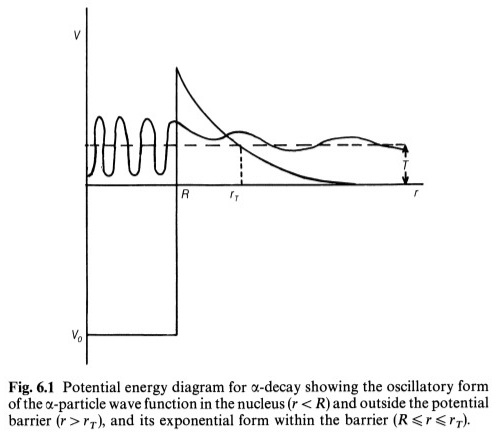
\includegraphics[width=4.5in]{immagini/potential_alpha.jpg} %immagine
\end{center}

L'idea è di una buca quadrata fino ad $r=R$ (raggio del nucleo), poi prevale il potenziale coulombiano. $r_T$ è il valore di $r$ per cui l'altezza della barriera coulombiana è uguale al valore dell'energia della particella $\alpha$; è il punto in cui la particella $\alpha$ esce dalla barriera.

\textbf{Tra $R$ e $r_T$ la funzione d'onda è del tipo esponenziale decrescente}. La zona tra $R$ e $r_T$ classicamente è la \textbf{zona proibita}. La probabilità di effetto tunnel è misurata dalla variazione di intensità di $R$ e $r_T$. Trascurando la parte angolare (o supponendo $l=0$) si ha:
\begin{equation}\begin{split}
\psi \left(r\right)=\frac{u}{r} \Longrightarrow -\frac{\hbar ^2}{2\mu}\frac{\textrm{d}^2u}{\textrm{d}r^2}V\left(r\right)u=T_{\alpha}u.
\end{split}\end{equation}
Considerando un valore $u\left(r\right)=e^{-y\left(t\right)}$ si ha:
\begin{equation}\begin{split}
-\frac{\textrm{d}^2y\left(t\right)}{\textrm{d}r^2}+\left(\frac{\textrm{d}y}{\textrm{d}r}\right)^2=\frac{2\mu}{\hbar ^2}\left(V-T_{\alpha}\right).
\end{split}\end{equation}
Se si suppone $y\sim r$, si ha $\frac{\textrm{d}^2y}{\textrm{d}r^2}=0$ e quindi:
\begin{equation}\begin{split}
\frac{\textrm{d}y}{\textrm{d}r}\sim\left[\frac{2\mu\left(V-T_{\alpha}\right)}{\hbar ^2}\right]^{\frac{1}{2}}\\
\Longrightarrow y\left(r\right)=\int{\left[\frac{2\mu\left(V-T_{\alpha}\right)}{\hbar ^2}\right]^{\frac{1}{2}}\textrm{d}r}
\end{split}\end{equation}

Interessante è il rapporto $$\frac{u\left(r_T\right)}{u\left(R\right)}\propto e^{-\gamma}$$ con
\begin{equation}\begin{split}
\gamma=\frac{1}{\hbar }\int{\left[2\mu\left(V-T_{\alpha}\right)\right]^{\frac{1}{2}}dr}
\end{split}\end{equation}
chiamato \textbf{coefficiente di Gamov}. La \textbf{penetrabilità della barriera} è data da:
\begin{equation}\begin{split}
T=\frac{\left|u\left(r_T\right)\right|^2}{\left|u\left(R\right)\right|^2}\propto e^{-2\gamma}
\end{split}\end{equation}
che è il \textbf{coefficiente di trasmissione}.

La \textbf{frequenza della particella $\alpha$} è, dentro il nucleo, quella con cui urta la barriera:
\begin{equation}\begin{split}
\nu=\frac{v}{2R}\sim 10^{21} \textrm{ Hz}\\
\lambda=e^{-2\gamma}\nu.
\end{split}\end{equation}

Con ipotesi superficiale ($T_{\alpha}\simeq 0$) si ha $$\gamma\sim \frac{8Ze^2}{4\pi\varepsilon \hbar v_{\alpha}}$$ e si ottiene
\begin{equation}\begin{split}
\ln{\left(\lambda\right)}=\ln{\left(\frac{v_i}{2R}\right)}-\frac{16Ze^2}{4\pi\varepsilon \hbar v_{\alpha}}\\
\Longrightarrow \ln{\left(\lambda\right)}=C+DT^{-\frac{1}{2}}_{\alpha}
\end{split}\end{equation}
con $C=\ln{\left(\frac{v_i}{2R}\right)}$ e $D=-\frac{16Ze^2}{4\pi\varepsilon \hbar}\sqrt{\frac{\mu}{2}}$.

\textbf{Il fattore $\gamma$ è grande ($\sim 50$): piccole variazioni nei parametri fanno variare molto il coefficiente di trasmissione}.

Il valore che si ottiene per la vita media dipende molto dai parametri (massa, raggio del nucleo, ...): può anche essere sfruttata per avere informazioni su questi parametri. \textbf{Si spiega così l'ampio range di variazione di $\tau$: $\gamma$ è molto sensibile a variazioni di massa e raggio}. Il parametro più incerto è $R$, e per ovviare al problema si utilizza $$R=r_0A^{\frac{1}{5}}$$ con $r_0=1.25$.

\section{Beta $\beta$} %β
\textbf{Si cambia il numero di neutroni e protoni nel nucleo}. Si parla di nuclei instabili per il rapporto tra neutroni e protoni. C'è una trasformazione di neutroni in protoni o viceversa; in particolare avviene:
\begin{equation}\begin{split}
n\longrightarrow p+e^-+\bar\nu_e \quad \textrm{\textbf{decadimento }}\beta^-\\
p\longrightarrow n+e^++\nu_e \quad \textrm{\textbf{decadimento }}\beta^+\\
p+e^-\longrightarrow n +\nu_e \quad \textrm{\textbf{cattura di elettrone}}
\end{split}\end{equation}

\textbf{Un neutrone singolo non è stabile, un protone singolo lo è}. In un tempo di vita medio di circa 15 minuti avviene il decadimento $\beta$: può avvenire anche per un neutrone libero. \textbf{Gli elettroni e i positroni non sono già nel nucleo, ma sono formati dal processo}.

\textbf{Ciò che cambia in questi processi è la carica Z del nucleo}: \ce{^A_ZX}

\textbf{A volte le reazioni vengono fatte su nuclei non stabili nello stato fondamentale. Il valore di Q deve essere ridotto}.

\begin{center}
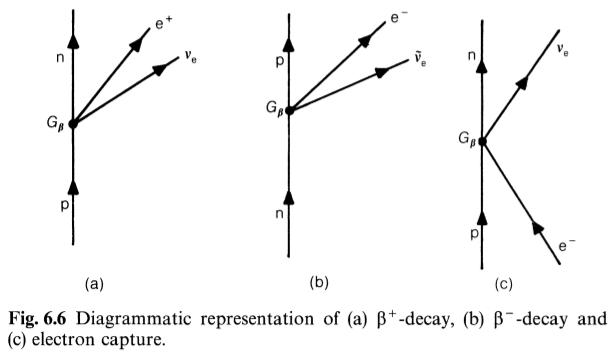
\includegraphics[width=4.5in]{immagini/beta-dacay.jpg} %immagine
\end{center}

\subsection{Decadimento $\beta^-$} %β-
\begin{equation}\begin{split}
\ce{^A_ZX}\longrightarrow \ce{^A_{Z+1}Y}+e^-+\bar\nu_e
\end{split}\end{equation}
Si suppongono due particelle e ci si aspetta uno spettro discreto per le energie degli elettroni (come disintegrazione a due corpi tipo il decadimento $\alpha$); invece \textbf{si osserva uno spettro continuo e un'apparente violazione della conservazione dell'energia}:
\begin{equation}\begin{split}
E_x=E_y+E_{e^-}=E_y+T_{e^-}+m_ec^2\\
\Longrightarrow T_{e^-}=\left(E_x-E_y-m_ec^2\right)=\left(M_x-M_y-m_e\right)c^2-T_y
\end{split}\end{equation}
indicando con $E_y$ l'energia di rinculo del nucleo $Y$. Il $Q$ della reazione, visto che $M_y\gg M_{e^-}$ e che $T_y\gg T_{e^-}$, andrebbe quasi tutto all'elettrone. \textbf{Lo spettro assunto è continuo, piccato sul valore atteso}, ma non una riga discreta sul valore di $T_{e^-}\simeq Q$ attesa.

\textbf{C'è anche un'apparente violazione della conservazione del momento angolare}: $A$ non cambia, il $J$ totale non cambia nel nucleo (sia $p$ che $n$ hanno spin $\frac{1}{2}$) ma è prodotto anche un $e^-$ anch'esso con spin $\frac{1}{2}$. Si avrebbe spin intero nello stato iniziale e spin semi-intero nello stato finale, se il nucleo avesse spin totale intero. Il fatto è che \textbf{viene in effetti prodotta un'altra particella}; essa deve avere massa molto piccola (cioè che non necessiti di molta energia per essere creata) così da non spostare lo spettro, non avere carica ed avere spin $\frac{1}{2}$. Ciò che aggiusta tutto questo è il \textbf{neutrino}. La sua massa è praticamente trascurabile ed ha una antiparticella.

\textbf{Nel decadimento quindi si produce l'antineutrino $\bar\nu_e$}.

\begin{equation}\begin{split}
M_xc^2=T_y+M_yc^2+T_{e^-}+m_ec^2+T_{\bar\nu}+m_{\bar\nu}c^2\\
\Longrightarrow Q=T_y+T_{e^-}+T_{\bar\nu}=\\
=\left(M_x-M_y-m_e-m_{\bar\nu}\right)c^2=\left[M\left(A,Z\right)-M\left(A,Z-1\right)\right]c^2
\end{split}\end{equation}
\textbf{Per avere la reazione deve essere $Q>0$}.

\paragraph{Scoperta del neutrino} Il neutrino, postulato da Pauli, fu trovato nel 1956, in un esperimento che coinvolgeva un reattore di fissione (grande produttore di neutroni liberi che poi decadono $\beta^-$ emettendo antineutrini). Si usò un rivelatore con acqua per sfruttare la reazione inversa $$\bar\nu_e+p\longrightarrow n+e^+.$$ La reazione però ha una sezione d'urto molto bassa. Il segnale era costituito da due fotoni ($\sim 0.5$ MeV) dati uno da annichilazione di $e^+$ con un elettrone, detta materia circostante, e l'altro da un altro fotone (più complesso), che compariva con un po' di ritardo, che era dato dal neutrone uscente dalla reazione che veniva assorbito da barre di cadmio che veniva eccitato e poi si diseccitava emettendo il fotone. \textbf{Viene supposta la presenza del neutrino $\nu$ perché l'energia dei fotoni non corrispondeva con quella aspettata}.

\subsection{Decadimento $\beta^+$} %β+
\begin{equation}\begin{split}
\ce{^A_ZX}\longrightarrow \ce{^A_{Z-1}Y}+e^++\nu_e
\end{split}\end{equation}
\begin{equation}\begin{split}
Q=\\
=\left[M_{\textrm{nucleo}}\left(A,Z\right)-M_{\textrm{nucleo}}\left(A,Z-1\right)-m_e\right]c^2=\\
=\left[M\left(A,Z\right)Zm_e-M\left(A,Z-1\right)+\left(Z+1\right)m_e-m_e\right]=\\
=\left[M\left(A,Z\right)-M\left(A,Z-1\right)-2m_e\right]c^2
\end{split}\end{equation}
\textbf{Per avere la reazione deve essere $Q>0$}.

\subsection{Cattura di elettrone} %Cattura di elettrone
\begin{equation}\begin{split}
e^-+\ce{^A_ZX}\longrightarrow \ce{^A_{Z-1}Y}+\nu_e
\end{split}\end{equation}
\begin{equation}\begin{split}
Q=\left[M\left(A,Z\right)-M\left(A,Z-1\right)\right]c^2
\end{split}\end{equation}

\textbf{Accade quando un nucleo assorbe uno dei suoi elettroni orbitanti e un protone del nucleo diventa un neutrone e come risultato si ottiene l’emissione di un neutrino}.

Può accadere che $Q$ sia positivo per l'energia cinetica ma non per $\beta^+$ perché c'è di mezzo il termine $2m_e$. Se $Q_{k}$ e $Q_{\beta}$ sono entrambi positivi, i due processi sono competitivi tra loro.

\textbf{A governare il processo c'è l'interazione nucleare debole}.

\textbf{Viene conservato il numero di nucleoni e il numero leptonico. Il decadimento $\beta$ non coinvolge un'interazione nucleare forte né quella elettromagnetica}.

\section{Gamma $\gamma$} %γ
Avvengono \textbf{transizioni nucleari}. Può essere generato un nucleo, a seguito di un decadimento $\alpha$ o $\beta$, che nello stato eccitato emette $\gamma$.

I $\gamma$ non sono carichi ma \textbf{hanno una natura elettromagnetica}, rivelata dalla diffrazione su cristalli da Rutherford e Andrade.

\begin{equation}\begin{split}
\textrm{raggi }x\longrightarrow \textrm{eV} \longrightarrow \lambda\sim10^{-1} \textrm{ m} \quad \textrm{transizioni atomiche}\\
\textrm{raggi }\gamma\longrightarrow \textrm{MeV} \longrightarrow \lambda\sim10^{-12}-10^{-15} \textrm{ m} \quad \textrm{transizioni nucleari}
\end{split}\end{equation}

\begin{center}
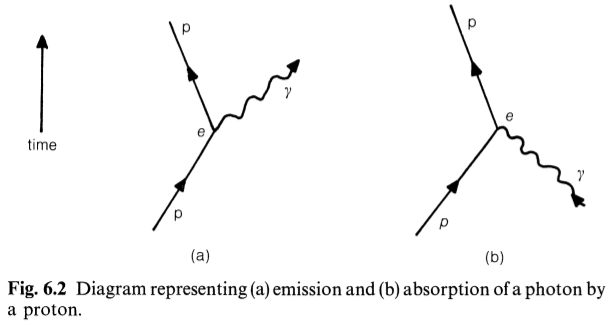
\includegraphics[width=4.5in]{immagini/gamma-dacay.jpg} %immagine
\end{center}

\begin{equation}\begin{split}
\left(A,Z\right)^+\longrightarrow \left(A,Z\right)+\gamma
\end{split}\end{equation}

\textbf{Il nucleo rimane inalterato, è l'energia a variare}. Un $\gamma$ porta informazioni sull'energia degli stati nucleari. \textbf{Un $\gamma$ può essere assorbito o emesso} ed energeticamente si ha:
\begin{equation}\begin{split}
h\nu=\mp\left(E_i-E_f\right)
\end{split}\end{equation}
considerando il segno ``meno'' per l'assorbimento e il segno ``più'' per l'emissione.

\textbf{Si conserva la quantità di moto} in quanto avviene un rinculo del nucleo:
\begin{equation}\begin{split}
\frac{h\nu}{c}=Mv\\
\Longrightarrow E_i-E_f=\mp h\nu+\frac{1}{2}Mv^2=\mp h\nu+\frac{1}{2M}\left(\frac{h\nu}{c}\right)^2\\
\Longrightarrow h\nu=\mp\left(E_i-E_f-\frac{h^2\nu^2}{2M c^2}\right)
\end{split}\end{equation}
avendo considerato $v$ la velocità di rinculo, $\Delta E_r=\frac{h^2\nu^2}{2M c^2}$ l'energia di rinculo ed $M$ la massa. Imponendo poi $\Delta E=E_i-E_f$, $\Delta t=\tau$ si ha $$\tau\Delta E\sim \hbar \Longrightarrow \Delta E\sim \frac{\hbar }{\tau}$$ si ha quindi
\begin{equation}\begin{split}
\Delta E_r\gg\Delta E
\end{split}\end{equation}

\paragraph{Esempio} Un atomo con $A=50$ ha \textbf{a livello atomico} $h\nu=1$ eV, $Mc^2=5\cdot 10^4$ MeV e quindi $$\Delta E_r=10^{-11} \textrm{ eV}$$ $\tau=10^{-8}$ s, $$\Delta E=6.6\cdot 10^{-8} \textrm{ eV.}$$ Grazie a questo si nota che
\begin{equation}\begin{split}
\Delta E_r\ll\Delta E
\end{split}\end{equation}
\textbf{per transizioni atomiche può avvenire assorbimento risonante}.

\textbf{Nel nucleo} invece, si ha $h\nu=10^5$ eV, $Mc^2=5\cdot 10^{4}$ MeV, $$\Delta E_r=10^{-1} \textrm{ eV}$$ e con $\tau=10^{-17}$ s si ha $$\Delta E=6.6\cdot 10^{-4} \textrm{ eV,}$$ cioè
\begin{equation}\begin{split}
\Delta E_r\gg\Delta E
\end{split}\end{equation}
e perciò \textbf{non è possibile l'assorbimento risonante nel nucleo}.

In realtà si può avere se si riduce $\Delta E_r$, il fattore di rinculo, aumentando la massa, ad esempio "congelando" il nucleo in un reticolo cristallino rigido. Così si hanno informazioni sui livelli nucleari. Il rinculo è minimo perché è relativo all'intero cristallo che ha massa molto grande.

\chapter{Accleratori} %Accleratori
Importante per tutti gli acceleratori è la \textbf{forza elettromagnetica}:
\begin{equation}\begin{split}
\vec F=\frac{d\vec p}{dt}=q\left(\vec E+\vec v \times \vec B\right)
\end{split}\end{equation}
dove il primo termine tra parentesi modifica la velocità mentre il secondo la direzione.

Per il trasporto del fascio sono necessari:
\begin{itemize}
\item \textbf{collimatori};
\item \textbf{deflettori};
\item \textbf{lenti magnetiche}.
\end{itemize}
Si stanno ora sviluppando delle tecniche a vuoto, per evitare che i fasci incontrino ostacoli e ci siano dispersioni. Gli acceleratori si dividono in:
\begin{itemize}
\item a bersaglio fisso (fisica nucleare);
\item a collisione di fasci (fisica subnucleare).
\end{itemize}
Inoltre sono di tre tipi:
\begin{itemize}
\item elettrostatici;
\item ciclici;
\item circolari.
\end{itemize}

\begin{center}\begin{tabularx}{\textwidth}{lXX}
\toprule
Tipo di acceleratore & Particelle accelerate & Energia massima o d.d.p.\\
\midrule
\textbf{Acceleratori continui} &  & \\
Cockroft-Walton & Qualsiasi & $\simeq 5$ MV\\
Van der Graaff & Qualsiasi & $\simeq 20$ MV\\
Van der Graaff tandem & Ioni negativi & $\simeq 40$ MV\\
Betatrone & $e$ & $\simeq 400$ MeV\\
LINAC & $e$ & $\simeq 50$ GeV\\
\midrule
\textbf{Acceleratori a frequenza} &  & \\
Acceleratori lineari & Qualsiasi & $\simeq 800$ MeV\\
Ciclotrone semplice & Qualsiasi & $\simeq 22$ MeV\\
Ciclotrone sector-focusing & Qualsiasi & $\simeq 500$ MeV\\
Sincrociclotrone & Qualsiasi & $\simeq 1000$ MeV\\
Sincrotrone a protoni & Qualsiasi & $\simeq 900$ GeV\\
Sincrotrone a elettroni & $e$ & $\simeq 100$ GeV\\
\bottomrule
\end{tabularx}\end{center}

\section{Acceleratori a caduta di potenziale} %Acceleratori a caduta di potenziale
\subsection{Cockroft-Walton} %Cockroft-Walton
Il generatore Cockcroft-Walton o moltiplicatore di tensione è un apparecchio che permette di convertire della corrente elettrica alternata o continua a bassa tensione in corrente continua ad alta tensione.

\textbf{Il moltiplicatore vero e proprio è ottenuto dalla serie di più moduli di livellamento, composti da capacità e diodi, in modo da ottenere un effetto di smorzamento dell'oscillazione iniziale unito ad un'amplificazione della tensione in ingresso}. I moltiplicatori sono caratterizzati in base al numero di stadi che li compongono ovvero il numero di condensatori tra la terra e l'uscita $V_{out}$.

Se il trasformatore inizialmente fornisce $V<0$, $D_2$ è bloccato e la corrente scorre solo attraverso $D_1$, andando a caricare il condensatore in alto nella figura, fino al potenziale di picco $V_p$. Quando la corrente si inverte, $D_1$ è bloccato e la corrente transita per $D_2$, andando a caricare il condensatore $C$ in basso ad un potenziale che è la somma di quello del trasformatore e di quello sull'altro $C$. In questo modo la tensione finale sul condensatore in basso è $V_{out}=2V_p$, che è appunto la tensione in uscita dal moltiplicatore.

\begin{center}
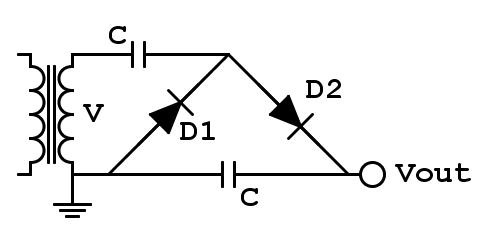
\includegraphics[width=2.5in]{immagini/Cockroft-Walton.jpg} %immagine
\end{center}

Il fatto che la tensione  cresca come $n^3$ implica che ci sono crescenti distorsioni nel segnale in uscita all'aumentare del numero di stadi usati nel moltiplicatore, fino al punto che $V_{out}$ non può più essere approssimata come tensione continua. Ciò limita nella pratica la possibilità di costruire dispositivi con un numero di stadi troppo elevato, a meno di prendere particolari accorgimenti. Ad esempio, invece di prendere condensatori con capacità uguali, la scelta di mettere condensatori con capacità grandi alla base del circuito permette di attutire questo effetto distorsivo. Anche l'invio di tensioni con forma d'onda quadra o triangolare permette di mantenere la tensione in uscita approssimativamente continua.

\subsection{Van der Graaff} %Van der Graaff
Elettrodo caricato per induzione elettrostatica. Il generatore di Van de Graaf è un generatore elettrostatico in grado di accumulare una notevole quantità di carica elettrica in un conduttore, creando tra questo ed un elettrodo di riferimento, solitamente messo a terra, un'altissima tensione (si può arrivare fino a milioni di Volt).

Un generatore di questo tipo è composto sostanzialmente da una cinghia di materiale isolante (caucciù) tesa tra due pulegge e mantenuta in rotazione da un motore. La cinghia viene caricata per induzione da una serie di punte metalliche (effetto punta) poste in prossimità di una delle due pulegge e collegate ad un generatore di tensione continua (ad esempio una batteria).

Queste cariche vengono poi trasportate, per azione del motore, all'interno di un conduttore di forma sferica isolato, dove un secondo pettine metallico collegato elettricamente alla sfera le trasferisce sulla superficie di quest'ultima. Se non si spegne la macchina il processo si arresta quando la tensione della sfera è sufficiente a produrre scariche elettriche attraverso gli isolanti di sostegno (rottura dielettrica) o attraverso l'aria circostante (ionizzazione dell'aria). Il tipico esperimento che si fa nelle scuole è quello di avvicinare alla sfera in tensione un conduttore posto a massa e di osservare la scarica che si genera in modo analogo ai fulmini.

\textbf{Il massimo potenziale raggiunto da un acceleratore Van de Graaff è pari a 25,5 MV}.

\begin{center}
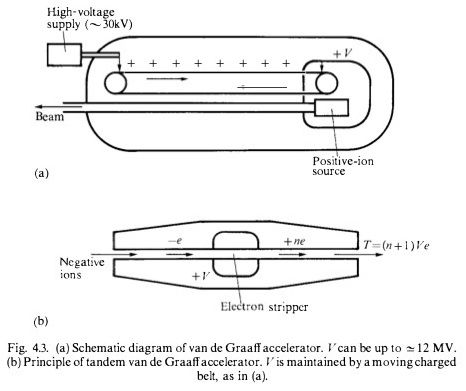
\includegraphics[width=4in]{immagini/acc_potential.jpg} %immagine
\end{center}

\subsection{Van der Graaff tandem} %Van der Graaff tandem
Ha lo stesso funzionamento del Van der Graaff normale ma si hanno acceleratori a più stadi (d.d.p. di circa 40 MV).

Il più recente sviluppo del generatore di Van de Graaff è stato, a partire dal 1958, l'acceleratore a bersaglio fisso, elettrostatico, tipo tandem. Alcuni ioni negativi (generalmente ioni idrogeno con due elettroni) vengono emessi da una sorgente, collimati ed immessi in un tubo di pochi metri ai cui estremi si trovano un elettrodo a terra ed un elettrodo con potenziale positivo prodotto da un generatore di Van de Graaff. Gli ioni negativi vengono così accelerati verso l'elettrodo ad alta tensione, dove un getto di idrogeno li libera dagli elettroni. Gli ioni positivi così ricavati vengono quindi ulteriormente accelerati verso il bersaglio fisso costituito dall'elettrodo a terra.

\section{Acceleratori lineari} %Acceleratori lineari

\begin{center}
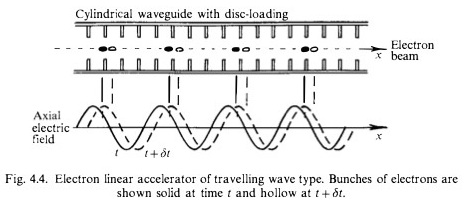
\includegraphics[width=5in]{immagini/linac.jpg} %immagine
\end{center}

Gli acceleratori lineari di particelle (o LINAC, da lin(ear) ac(celerator)) sono strutture in grado di accelerare particelle cariche (protoni, elettroni, positroni, ioni pesanti, ...), generate per mezzo di un cannone termoionico, un fotoiniettore o altri mezzi.

\subsection{LINAC} %LINAC
Il tempo che la particella passa nel tubo deve essere $\frac{T}{2}$, con $T$ il periodo del potenziale ottenuto. \textbf{Più le particelle sono stabili, più il tubo deve essere lungo}: $$L_n=v_n\frac{T}{2}.$$ C'è una polarità alternata degli elettrodi.

\begin{center}
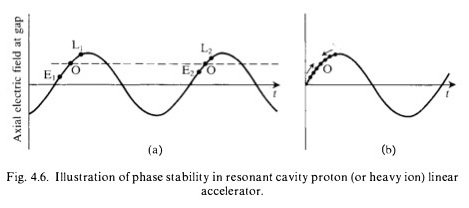
\includegraphics[width=5in]{immagini/linac_2.jpg} %immagine
\end{center}

I tubi fanno da gabbie di Farady e contemporaneamente da acceleratori, grazie alla polarità alternata. \textbf{Le particelle accelerano fuori dai tubi, all'interno infatti il campo elettrico è nullo}. I più moderni acceleratori lineari sono a guide d'onda.

Il compito di un LINAC storicamente è quello di creare un fascio idoneo ad essere iniettato in un acceleratore circolare (in cui ottenere collisioni per studi di fisica delle alte energie), o in anelli di accumulazione (ad es. per luce di sincrotrone). Più recentemente i LINAC vengono utilizzati per scopi medicali, quali terapia antitumorale. Il fascio di elettroni prodotto nella guida acceleratrice può essere utilizzato per il trattamento diretto o per colpire un bersaglio, al fine di produrre raggi X. I raggi X vengono utilizzati per il trattamento di neoplasie profonde, dato il loro alto potere di penetrazione, mentre i fasci di elettroni per la terapia di neoplasie superficiali, data la proprietà di cedere la loro energia in maniera uniforme in tessuti spessi pochi centimetri.

Coppie di acceleratori lineari di più alta energia sono utilizzati direttamente per generare collisioni di particelle, ad esempio a SLAC.

LINAC di alta intensità vengono utilizzati come iniettori per i Free Electron Laser.

\section{Acceleratori circolari} %Acceleratori circolari
Si utilizzano anche campi magnetici.

\subsection{Ciclotrone} %Ciclotrone
\textbf{Un ciclotrone è una macchina usata per accelerare fasci di particelle elettricamente cariche (normalmente ioni leggeri) utilizzando una corrente alternata ad alta frequenza ed alta tensione, in associazione con un campo magnetico perpendicolare}.

La traiettoria percorsa dalle particelle è a spirale a partire dal centro. Raggiunto il bordo esterno della macchina il fascio fuoriesce ad alta velocità, prossima alla velocità della luce.

\textbf{Il principio sfruttato è la risonanza ionica ciclotronica}. All'interno della camera a vuoto circolare sono presenti due elettrodi semicircolari cavi a forma di D. I due elettrodi sono come due gusci accostati per le aperture (la parte piatta della D). Questi elettrodi possono essere colpiti da particelle spurie che ne causano il riscaldamento e devono essere raffreddati mediante circolazione di acqua in appositi tubi. La camera è posta tra le espansioni polari di un potente magnete, in modo che il campo attraversi il piano su cui giacciono gli elettrodi. Quando una particella viene introdotta tangenzialmente alla camera, ortogonalmente al campo magnetico, essa viene deviata e mantenuta su un'orbita circolare per effetto della forza di Lorentz. Nel vuoto la particella è libera di ruotare, ma, perdendo lentamente energia (tutte le cariche elettriche, se accelerate, emettono fotoni, detti di Bremsstrahlung), percorre una traiettoria a spirale fino al centro.

Se ora viene applicata una opportuna differenza di potenziale alternata ad alta frequenza tra i due elettrodi, le particelle subiscono un'accelerazione ogni volta che passano nello spazio tra essi. Accelerando, il diametro dell'orbita aumenta, fino a quando il fascio non fuoriesce tangenzialmente dal bordo del dispositivo.

La forza centripeta che trattiene le particelle nella traiettoria circolare è generata dal campo magnetico trasversale B per effetto della forza di Lorentz. L'entità della forza equivale a $qvB$, quindi:
$$q\vec v\vec B=m\frac{v^2}{\vec r}\Longrightarrow \vec r=\frac{m\vec v}{q\vec B}=\frac{\vec p}{q\vec B} \Longrightarrow \vec\omega =\frac{q\vec B}{m}$$
\textbf{Il ciclotrone lavora ad $\omega $ fissi}.

\begin{center}
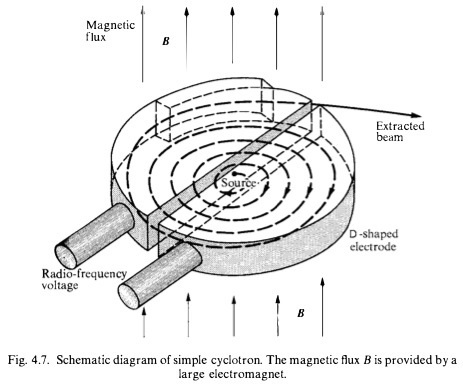
\includegraphics[width=5in]{immagini/ciclotron.jpg} %immagine
\end{center}

\begin{equation}\begin{split}
v_{\max}=\frac{qBr}{m}\\
\frac{1}{2}mv^2_{\max}=\frac{q^2B^2r^2}{2m}
\end{split}\end{equation}
Bisogna avere raggi grandi e che una maggiore d.d.p. non cambi la $v_{\max}$ (riduce al massimo il minimo di giri da fare se è alta). \textbf{Questa traiettoria va bene per particelle non relativistiche}. Non va bene per gli elettroni.

Per velocità relativistiche $m=\gamma m_0$ con $\gamma=\sqrt{1-\frac{v^2}{c^2}}$: $$\frac{d\vec p}{dt}=\vec\omega \times\vec p=\vec\omega \times m_0\gamma\vec v.$$

La frequenza $\nu=\frac{\omega }{2\pi}$ non è più costante. Si nota una radiofrequenza variabile. Per questo nascono i sincrociclotroni.

\textbf{Le particelle sono accelerate in pacchetti}. \textbf{Nel gap tra le due D del ciclotrone e il punto di immissione delle particelle c'è un effetto di focalizzazione temporale}.

Il ciclotrone è stato progettato con l'intenzione di superare le limitazioni dell'acceleratore lineare. All'epoca non era possibile generare onde radio contemporaneamente ad alta frequenza ed alta potenza, per cui gli stadi di accelerazione dovevano essere spaziati tra loro (per avere il tempo di cambiare il potenziale dell'elettrodo prima dell'arrivo della particella) oppure erano necessari più stadi (per compensare la limitata potenza). Per ottenere energie elevate era necessario costruire acceleratori lunghi e oltre un certo limite troppo costosi. Successivamente gli acceleratori lineari poterono disporre di maggiore potenza, ma il ciclotrone è comunque più conveniente.

\textbf{Nel ciclotrone il raggio è limitato dalla dimensione della camera cilindrica in cui le particelle si allargano a spirale dal centro}. Il campo magnetico prodotto da un magnete ordinario ed è limitato dalla saturazione del materiale, raggiunta quando tutti i domini magnetici sono allineati. La disposizione di coppie di magneti ordinari lungo tutta la traiettoria di un acceleratore comporterebbe costi elevati.

\subsection{Sincrotrone} %Sincrotrone
\textbf{Si varia nel tempo sia $B$ sia $V$}. L'orbita delle particelle è costante e non c'è una spirale di orbite ma una sola orbita. \textbf{Aumenta ad ogni passaggio l'energia e perciò bisogna aumentare la frequenza. Per mantenere il raggio costante occorre aumentare $B$}.

Il sincrotrone deriva dal ciclotrone, nel quale è utilizzato un campo magnetico costante ed un campo elettrico alternato a frequenza costante. Una variante è il sincrociclotrone, dove il campo magnetico oppure la frequenza del campo elettrico sono variabili in funzione dell'aumentare dell'energia posseduta dalle particelle.

Nel sincrotrone, entrambi i campi sono controllati in modo da mantenere l'orbita del fascio di particelle all'interno di un contenitore a forma toroidale cavo all'interno del quale sia stato praticato il vuoto. Nella pratica, per macchine di raggio maggiore, vengono usate brevi sezioni diritte, per cui la forma complessiva è poligonale con spigoli arrotondati. \textbf{Ad ogni angolo è presente un magnete per curvare la traiettoria del fascio}.

\begin{center}
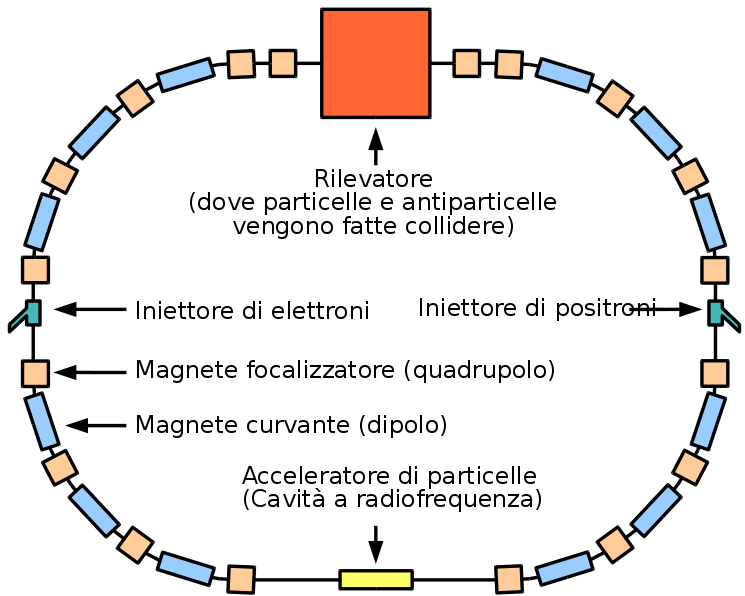
\includegraphics[width=4.5in]{immagini/sincrotron.jpg} %immagine
\end{center}

\textbf{L'energia massima ottenibile da un acceleratore circolare è limitata dall'intensità dei campi magnetici e dal raggio massimo dell'orbita delle particelle}.

Nei sincrotroni le limitazioni del ciclotrone sono superate utilizzando fasci molto stretti focalizzati da magneti piccoli ma il cui campo è molto focalizzato. \textbf{Il limite di energia applicabile al fascio} è determinato dal fatto che una particella carica soggetta ad accelerazione emette energia sotto forma di fotoni. Quando l'energia persa per emissione elettromagnetica equivale a quella fornita ad ogni ciclo, il fascio non può essere ulteriormente accelerato. Questo limite viene aumentato costruendo acceleratori di raggio maggiore e aggiungendo ad ogni tratto rettilineo numerose cavità a microonde in grado di accelerare ulteriormente il fascio. Le particelle più leggere (per esempio gli elettroni) perdono una frazione maggiore di energia, per questo negli acceleratori più grandi vengono usate particelle cariche pesanti, come protoni e nuclei atomici.

\subsection{Betatrone} %Betatrone
\textbf{Viene utilizzato per accelerare elettroni}. Il betatrone è costituito da due espansioni polari circolari che generano un campo magnetico variabile nel tempo a simmetria radiale. All'interno è posto un toroide cavo al cui interno è praticato il vuoto in modo che le particelle non impattino con molecole d'aria durante la fase di accelerazione.

\begin{center}
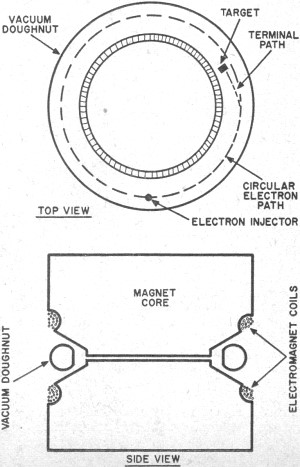
\includegraphics[width=2.5in]{immagini/betatron.jpg} %immagine
\end{center}

Le particelle da accelerare vengono immesse all'interno della cavità toroidale. Essendo il campo magnetico variabile nel tempo si ha un campo elettrico indotto non conservativo come descritto dalle equazioni di Maxwell. Il campo elettrico indotto accelera la particella carica mentre il campo magnetico ha la funzione di defletterla, tramite la forza di Lorentz, per mantenerla in un'orbita circolare. \textbf{Le cariche possono acquistare un'energia cinetica di 150 MeV} (al loro raggiungimento un elettrone compie \si{150.000} giri in 0.0032 s). Raggiunta la massima energia, le cariche elettriche vengono deviate in una regione di spazio in cui un altro campo magnetico provvede a curvare le traiettorie verso l'esterno.

L'energia massima di un betatrone è in parte limitata dalla potenza del campo magnetico (dovuta alla grandezza del magnete).

\textbf{Nel betatrone si parla solo di campo magnetico}. Più gli elettroni sono veloci più il campo $B$ deve aumentare proporzionalmente all'energia delle particelle per mantenere il raggio.

\paragraph{Condizione di betatrone} Una particella di carica $q$ è soggetta alla forza tangenziale $$\frac{d\vec p}{dt}=q\vec E=\frac{q}{2}\vec r\times \frac{d\vec \langle B\rangle}{dt}.$$ Affinché la particella percorra la circonferenza di raggio $R$ costante, deve risultare
\begin{equation}\begin{split}
\frac{d\vec p}{dt}=q\vec r\times \frac{dB_0}{dt}
\end{split}\end{equation}
Quindi è possibile accelerare un elettrone lungo una traiettoria di raggio costante se è soddisfatta la
\textbf{condizione di betatrone}
\begin{equation}\begin{split}
\frac{d\langle \vec B\rangle}{dt}=2\frac{dB_0}{dt}\\
\Longrightarrow \langle \vec B\rangle=2B_0+\textrm{const}
\end{split}\end{equation}
che si può ottenere sagomando opportunamente i poli del magnete.

\section{Reazioni per ottenere neutroni} %Reazioni per ottenere neutroni
Per ottenere neutroni si possono utilizzare diversi metodi:
\begin{itemize}
\item attraverso la fissione nei reattori nucleari;
\item $p+A\longrightarrow n$, con $A$ nucleo pesante;
\item $\alpha+\ce{^9_4Be}\longrightarrow \ce{^{12}_6C}+n$;
\item $\alpha+\ce{^{11}_6B}\longrightarrow \ce{^{14}_7N}+n$.
\end{itemize}

\chapter{Rivelatori} %Rivelatori
Nello scattering si avranno dei prodotti che però tenderanno a ricombinarsi, quindi uno degli scopi fondamentali consiste nel tener separate le particelle che produce la reazione.

\textbf{La rivelazione di una particella avviene grazie alla conoscenza di come la singola particella interagisce con la materia}.

Le particelle, interagendo, perdono man mano energia, tramite interazione con altri elettroni di atomi costituenti la materia o addirittura ionizzandoli.

Considerando un urto tra una particella di massa $M$ e velocità $v$ con un elettrone fermo si ha:
\begin{equation}\begin{split}
\begin{cases}
E=\frac{1}{2}Mv^2=\frac{1}{2}Mv^{2'}+\frac{1}{2}m_ev_e^2 & \Longrightarrow M\left(v-v'\right)\left(v+v'\right)=m_ev_e^2\\
Mv=Mv'+m_ev_e & \Longrightarrow M\left(v-v'\right)=m_ev_e
\end{cases}
\end{split}\end{equation}
\begin{equation}\begin{split}
v'=\frac{M-m_e}{M+m_e}v\\
v_e=\frac{2M}{M+m_e}v
\end{split}\end{equation}
essendo $M\gg m_e$ si ha in definitiva
\begin{equation}\begin{split}
v_e\sim 2v
\end{split}\end{equation}

Inserendo quanto trovato nella formula dell'energia cinetica si ha:
\begin{equation}\begin{split}
\frac{1}{2}mv_e^2=4\frac{m_e}{M}E
\end{split}\end{equation}

Ioni ed elettroni danno poi segnali elettrici che possono essere usati per dare ulteriori informazioni.

\paragraph{Formula di stopping-power} Viene chiamata anche di Bethe-Bohr. Un parametro fondamentale nella rivelazione è il \textbf{rate di perdita di energia di una particella che interagisce con la materia}. Viene formulata come segue:
\begin{equation}\begin{split}
-\frac{dE}{dx}=\left(\frac{ze^2}{4\pi\varepsilon_0}\right)^2\frac{4\pi Z\rho N_A}{Amv^2}\left[\ln{\left(\frac{2mv^2}{I}\right)}-\ln{\left(1-\beta^2\right)}-\beta^2\right]
\end{split}\end{equation}
considerando $\beta=\frac{v}{c}$, $z$ il numero di cariche nella particella, $Z$ il numero di cariche degli atomi del materiale con cui c'è interazione, $N_A$ il numero di Avogadro, $A$ il numero di massa del materiale, $\rho$ la densità del materiale, $I$ l'energia media di ionizzazione per gli atomi del mezzo.

Si nota quindi che l'energia trasferita è inversamente proporzionale alla velocità al quadrato:
\begin{equation}\begin{split}
E\propto \frac{1}{v^2}
\end{split}\end{equation}

\begin{center}
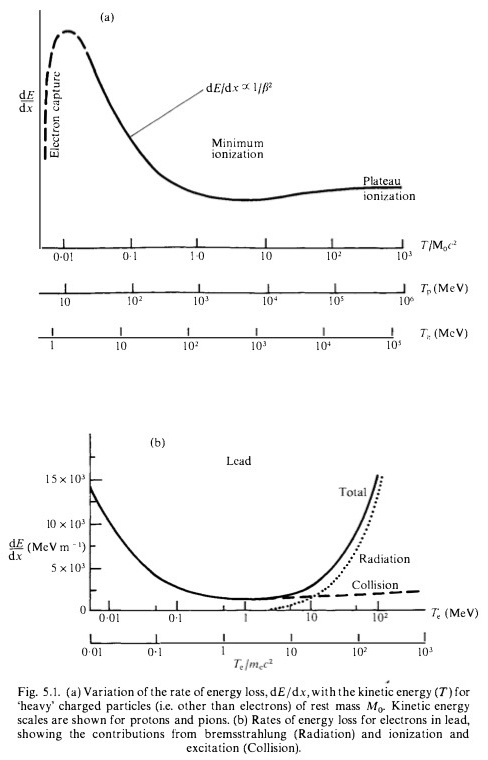
\includegraphics[width=4.5in]{immagini/stopping_power.jpg} %immagine
\end{center}

Il \textbf{range di una particella}, cioè la distanza percorsa con perdita di tutta l'energia è:
\begin{equation}\begin{split}
R=\int{\frac{dx}{dE}dE}
\end{split}\end{equation}
\textbf{La perdita di energia ha un minimo alla fine del percorso}.

\section[Interazioni]{Interazione tra radiazione e materia} %Interazione tra radiazione e materia
\textbf{Con emissione di radiazioni avviene una perdita di energia}. Si ha
\begin{equation}\begin{split}
\left(-\frac{dE}{dt}\right)_{\textrm{rad}}\propto \frac{q^2Z^2}{M^2}E_k
\end{split}\end{equation}
con $E_k$ l'energia cinetica della particella incidente. Oltre i 10 MeV di energia dell'elettrone incidente questi diventa il contributo dominante.

\textbf{I neutroni perdono energia per collisioni con i nuclei} ma non sentono l'interazione coulombiana. Si mostra che, ad energie non relativistiche, l'energia massima trasferita con un urto frontale con un nucleo di massa $A$ è
\begin{equation}\begin{split}
E_{\max}=\frac{4T_0A}{\left(A+1\right)^2}
\end{split}\end{equation}

Per quanto riguarda il \textbf{fotone} esso risente di tre effetti (fotoelettrico, Compton, produzione di coppie). Viene definito il \textbf{coefficiente di assorbimento efficace} come
\begin{equation}\begin{split}
\mu=\mu_{\textrm{fotoel}}+\mu_{\textrm{Compton}}+\mu_{\textrm{coppie}}
\end{split}\end{equation}
L'\textbf{intensità dei fotoni} invece è definita come
\begin{equation}\begin{split}
I\left(x\right)=I_0e^{-\mu x}
\end{split}\end{equation}
mentre l'\textbf{emispessore} è
\begin{equation}\begin{split}
x_{\frac{1}{2}}=\frac{\ln{\left(2\right)}}{\mu}.
\end{split}\end{equation}

\subsection{Effetto fotoelettrico} %Effetto fotoelettrico
\textbf{Un fotone è assorbito dall'elettrone di un atomo, che può essere promosso a livelli superiori, o addirittura può liberarsi dall'atomo ed uscire}. L'energia del fotone deve essere maggiore di $|I_b|$.

\begin{center}
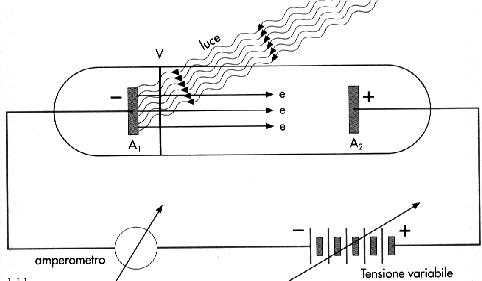
\includegraphics[width=5in]{immagini/photoelectric.jpg} %immagine
\end{center}

In fisica dello stato solido l'effetto fotoelettrico è il fenomeno fisico caratterizzato dall'emissione di elettroni da una superficie, solitamente metallica, quando questa viene colpita da una radiazione elettromagnetica, ossia da fotoni aventi una certa lunghezza d'onda.

Come comprese Einstein, riprendendo la teoria di Planck, l’effetto fotoelettrico evidenzia la natura quantistica della luce. Nella radiazione elettromagnetica l’energia non è distribuita in modo uniforme sull’intero fronte dell’onda ma concentrata in singoli quanti (pacchetti discreti) di energia, i fotoni, e ogni fotone interagisce singolarmente con un elettrone, al quale cede la sua energia. Affinché si verifichi è necessario che il fotone abbia un’energia sufficiente a rompere il legame elettrico che tiene legato l’elettrone all’atomo.

In altri termini \textbf{l’elettrone può uscire dal metallo solo se l’energia del fotone è almeno uguale al lavoro di estrazione ($h\nu \ge W_0$)}. Esiste, pertanto, una soglia minima di estrazione per ogni metallo, che fa riferimento o alla lunghezza d’onda o alla frequenza del fotone incidente e, quindi, alla sua energia $h\nu$, la quale coincide con il lavoro di estrazione ($W_0$).

\begin{equation}\begin{split}
E=h\nu=h\frac{c}{\lambda}=I_b-T_e.
\end{split}\end{equation}
$T_e$ è l'energia cinetica dell'elettrone uscente.

\textbf{Con l’aumentare dell’energia dei fotoni incidenti aumenta anche l’energia cinetica degli elettroni estratti. Le energie in gioco sono dell'ordine del KeV}.ick

\subsection{Effetto Compton} %Effetto Compton
\textbf{Il fotone ha energia maggiore dell'energia di legame. Il processo è descritto come urto elastico fra frequenza ed elettrone}: effetto fotoelettrico per un elettrone libero. \textbf{L'energia del fotone è dell'ordine del MeV}.

\begin{center}
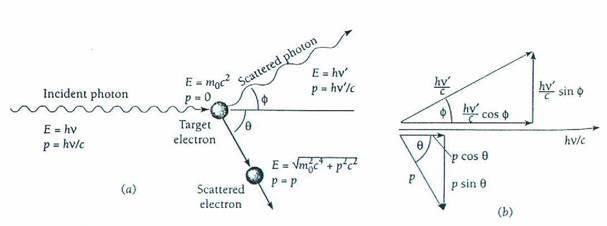
\includegraphics[width=\textwidth]{immagini/compton.jpg} %immagine
\end{center}

\begin{equation}\begin{split}
E_{\gamma}=h\nu\\
p_{\gamma}=\frac{E_{\gamma}}{c}
\end{split}\end{equation}
\begin{equation}\begin{split}
p_1+p_2=p'_1+p'_2 \Longrightarrow \\
\left(p'_2\right)^2=M^2=\left(p_1+p_2-p'_1\right)^2=p_1^2+p_2^2+{p'_1}^2+2p_1p_2-2p_1p'_1-2p_2p'_1=\\
=m^2+M^2+m^2+2ME-2ME'-2EE'+2pp'\cos{\left(\theta\right)} \Longrightarrow \\
m^2+ME-EE'-E'M+pp'\cos{\left(\theta\right)}=0
\end{split}\end{equation}
Essendo $m=0$ per il fotone, si ha:
\begin{equation}\begin{split}
E' \left[E\left(1-\cos{\left(\theta \right)}\right)+M\right]=EM \Longrightarrow \\
E' =\frac{EM}{1+\frac{E}{M}\left(1-\cos{\left(\theta \right)}\right)} \Longrightarrow \\
\lambda'=\lambda+\frac{h}{Mc}\left(1-\cos{\left(\theta \right)}\right) \Longrightarrow \\
\nu'=\frac{\nu}{1+\frac{h\nu}{Mc^2}\left(1-\cos{\left(\theta\right)}\right)}
\end{split}\end{equation}

Si vede quindi che \textbf{l'energia del fotone finale è minore di quella iniziale}, in quanto una parte di essa si è trasferita nell'$e^-$.

\subsection{Produzione di coppie} %Produzione di coppie
\textbf{Il fotone genera due particelle di carica opposta (mantenendo la conservazione dell'energia). La sezione d'urto è proporzionale a $Z^2$}.

È possibile avere produzione di coppie da un fotone, ma solo se questo passa accanto ad un altro corpo (come ad esempio un nucleo atomico) con cui può interagire.

L'energia del raggio gamma incidente viene equamente ripartita nella particella e nella sua antiparticella corrispettiva. Per un'energia pari ad almeno 1.022 MeV la coppia formatasi sarà elettrone-positrone, come evidenziato nel 1932. Per energie di almeno 1.9 GeV (la massa del protone è 1836 volte superiore a quella dell'elettrone, per cui l'energia necessaria per creare una coppia protone-antiprotone dev'essere notevolmente superiore a quella richiesta per generare la coppia elettrone-positrone) si creeranno una coppia protone-antiprotone e, per energie ancora superiori, neutrone-antineutrone ed \ce{H}-anti \ce{H}.

Anderson, nel 1932, scoprì l'esistenza del positrone, già previsto teoricamente da Dirac nel 1930. James Chadwick, da alcune reazioni di fissione nucleare, scoprì l'esistenza di una nuova particella elementare costituente il nucleo: il neutrone, particella elettricamente neutra con una massa circa uguale a quella del protone (leggermente superiore). Il neutrone è la prima particella instabile che viene scoperta. Essa, al di fuori del nucleo, decade in un tempo di circa 11 minuti secondo la reazione:
\begin{equation}
n \longrightarrow p + e^- + \bar\nu_e.
\end{equation}

Sia l'antiprotone che il neutrino furono osservati solo molti anni dopo, rispettivamente nel 1955-56 (E. Segrè) e nel 1956 (F. Reines e C. Cowan); l'antineutrone fu osservato nel 1957 da Piccioni. L'antiatomo d'idrogeno è stato prodotto nel 1969 bombardando con protoni da 70 GeV nuclei di alluminio. Le particelle si riconoscono per l'opposta deflessione, o, nel caso di particelle neutre, per il senso di rotazione (lo spin differenzia il neutrone, $+\frac{1}{2}$, dall'antineutrone, $-\frac{1}{2}$).

Il caso più semplice è la creazione a partire da un raggio $\gamma$ (fotone). La reazione corrispondente è:$$\gamma \longrightarrow e^{+} + e^{-}.$$ Per questo processo è possibile calcolare la sezione d'urto totale, basandosi sui due corrispondenti diagrammi di Feynman del primo ordine che descrivono l'interazione: $$\sigma (M) = 4 \pi \frac {\alpha^2}{M^2} \left [ \left (1-8 \frac {m_e^4}{M^4} + 4 \frac {m_e^2}{M^2} \right ) \ln \left ( \frac {1+ \sqrt {1-4 \frac {m_e^2}{M^2}}}{1- \sqrt {1-4 \frac {m_e^2}{M^2}}} \right ) - \sqrt {1-4 \frac {m_e^2}{M^2}} \left ( 1+4 \frac {m_e^2}{M^2} \right ) \right ].$$

\textbf{Il processo inverso è detto annichilazione elettrone-positrone}. Generalmente un'annichilazione segue sempre una creazione di coppia, poiché l'antiparticella non può esistere nel nostro mondo materiale: un antielettrone, ad esempio, generatosi per creazione di coppia, non appena incontra un elettrone annichila producendo due raggi gamma che dipartono nella medesima direzione su versi opposti e ripartendosi l'energia totale di 1.022 MeV, ed ognuno dei due raggi gamma emergenti sarà di 0.511 MeV. I raggi gamma prodotti sono due perché la quantità di moto della particella e la quantità di moto dell'antiparticella non possono andar perdute. In pratica, la ``scomparsa'' della particella e della corrispettiva antiparticella può esser considerata come la sovrapposizione di un'onda con un'altra onda avente le medesime caratteristiche della precedente, ma sfasata di 90 gradi, il che porta all'elisione dell'onda.

\textbf{Le energie in gioco sono di 10 MeV}.

\section{Rivelatori} %Rivelatori
Molti rivelatori di particelle si basano su fenomeni di ionizzazione generati da particelle cariche che attraversano un mezzo:
\begin{equation}\begin{split}
\textrm{ionizzazione specifica}=\frac{\textrm{energia persa ogni ionizzazione}}{\textrm{energia necessaria per avere n coppie di ioni}}
\end{split}\end{equation}
la carica viene raccolta mentre gli ioni positivi e gli $e^-$ vengono tenuti separati.

Le ionizzazioni possono essere:
\begin{itemize}
\item \textbf{direttamente dipendenti dalla radiazione};
\item \textbf{secondarie}, cioè generate da altre ionizzazioni (ma hanno comunque un legame con quelle iniziali).
\end{itemize}

Gli apparati possono anche essere progettati per produrre fotoni e sfruttare l'effetto fotoelettrico. Quando si registrano ioni, vengono usate differenze di potenziale per tenere le cariche separate (per d.d.p. troppo elevate la misura è poco precisa)

\textbf{Per rivelare fotoni si sfruttano i meccanismi visti prima, a seconda delle energie}.

\textbf{Per i neutroni si guardano gli effetti delle reazioni nucleari}.

\paragraph{Caratteristiche rivelatori}
\begin{itemize}
\item \textbf{Potere risolutivo temporale e spaziale}: capacità di definire l'istante o il luogo di passaggio della particella
\item \textbf{Efficienza}
\item \textbf{Tempo di recupero} 
\item \textbf{Trigger}
\end{itemize}

I \textbf{contatori a ionizzazione} usano impulsi generati dalla radiazione e non sfruttano le ionizzazioni secondarie (gli impulsi non vengono moltiplicati). Hanno tempi di recupero rapidi, possono pertanto effettuare misure in rapida successione, e hanno una buona risoluzione in energia.

I rivelatori possono essere piani o cilindrici; nel rivelatore cilindrico il filo interno è l'anodo e la struttura circostante è pertanto il catodo. Le ionizzazioni avvengono perciò soprattutto vicino al filo dove il campo è più intenso. \textbf{Il conteggio è proporzionale e le cariche prodotte da ionizzazione secondaria sono proporzionali a quelle date dalla ionizzazione primaria}.

\subsection{Regioni dei rivelatori}
\paragraph{Regione di ionizzazione} \textbf{Il segnale dipende da $V$ e dalla $V_{\textrm{drift}}$ di deriva delle cariche nel mezzo}. In generale
\begin{equation}\begin{split}
V_{\textrm{drift}_{e^-}}\gg V_{\textrm{drift}_{\textrm{ioni}^+}}.
\end{split}\end{equation}
\textbf{$V$ deve essere abbastanza grande da contrastare la ricombinazione, così che la maggior parte delle particelle ionizzate sia rivelata e non si perdano informazioni}. Il rapporto segnale/rumore è basso e ciò porta ad un'elettronica complicata. Il tempo di recupero è piccolo; si ha una bassa $V$. Non ci sono ionizzazioni secondarie.

\paragraph{Regione proporzionale} \textbf{Se si continua ad aumentare $V$, può capitare che si verifichi ionizzazioni secondarie provocate dagli elettroni}. Si avranno ampiezze maggiori, ma si ha un segnale proveniente anche dalle ionizzazioni secondarie. Ciò non è un problema perché \textbf{il numero di eventi di ionizzazioni secondarie è proporzionale al numero di eventi delle primarie}. I rivelatori che lavorano in questa regione sono di forma cilindrica:
\begin{equation}\begin{split}
E\left(r\right)=\frac{V}{r\ln{\left(\frac{b}{a}\right)}}
\end{split}\end{equation}
con $b$ raggio elettrodo esterno e $a$ raggio elettrodo interno.

\paragraph{Regione Geiger} Se si aumenta ancora $V$, con ionizzazioni terziarie e via dicendo, \textbf{si perde la memoria del segnale finale}.

Esistono rivelatori per ogni regione di funzionamento

\subsection{Rivelatore a gas} %Rivelatore a gas
Si misurano le cariche prodotte per ionizzazione. \textbf{Se una particella che passa attraverso un gas ha un'energia sufficiente per ionizzarlo produce delle coppie elettrone-ione lungo la sua traccia}. Queste coppie possono essere raccolte usando un campo elettrico, che fa migrare gli elettroni verso l'anodo positivo, e gli ioni verso il catodo negativo. \textbf{La carica misurata in alcuni casi è proporzionale all'energia della particella}. Non c'è quindi proporzionalità. I guadagni sono alti e l'elettronica è semplice.

I rivelatori a gas si dividono in due grosse categorie: rivelatori a campo elettrico radiale e rivelatori a campo elettrico uniforme. Della prima categoria sono: camere a ionizzazione, contatori proporzionali, contatori Geiger-Müller. La camera a fili è un rivelatore simile al contatore proporzionale, ma con molti elettrodi ed è quindi sensibile alla posizione. Alla seconda appartengono: gli RPC rivelatori a elettrodi piani resistivi che hanno una elevata risoluzione temporale.

\subsection{Camera a multifili} %Camera a multifili
Una camera a multifili è un rivelatore di particelle che rivela la radiazione ionizzante usando le idee del contatore Geiger e del contatore proporzionale. A differenza di questi ultimi utilizzando più fili anodici \textbf{è in grado di misurare la traiettoria della particella primaria}.

\begin{center}
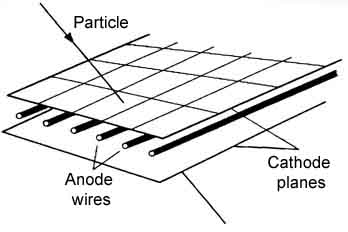
\includegraphics[width=3in]{immagini/multifili.jpg} %immagine
\end{center}

Il rivelatore è formato da molti fili paralleli, mantenuti ad alto potenziale positivo, tra due piani metallici mantenuti al potenziale di massa, paralleli ed equidistanti dal piano dei fili. Quando la particella interagisce con il gas contenuto nella camera lo ionizza creando coppie elettrone-ione positivo. Gli elettroni migrano verso il piano anodico e quando giungono in prossimità di un anodo si moltiplicano, creando una valanga. Andando a vedere quale anodo ha prodotto il segnale si può trovare una coordinata spaziale. La risoluzione spaziale è data dal tempo di raccolta della carica (cioè il tempo di deriva degli elettroni). Sono un insieme di contatori proporzionali.

\subsection{Camera a deriva (drift)} %Camera a deriva (drift)
La camera a deriva è un particolare tipo di camera proporzionale a multifili in cui le informazioni posizionali sulle particelle sono ottenute misurando il tempo necessario a raggiungere l'anodo da parte degli elettroni estratti dalle particelle stesse dagli atomi di gas utilizzato per riempire la camera. Per la definizione spaziale si misura il tempo di deriva degli elettroni; con segnali di riferimento temporale si sincronizza col passaggio del fascio.

\begin{center}
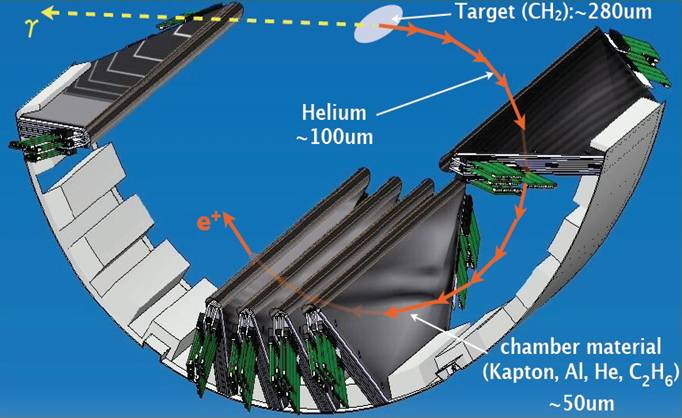
\includegraphics[width=5in]{immagini/drift.jpg} %immagine
\end{center}

\textbf{Nelle camere a drift si misura la velocità di deriva degli elettroni rispetto ad un riferimento esterno} (un trigger di solito dato da un altro rivelatore o da un segnale sincronizzato)

\subsection{Geiger-Müller} %Geiger-Müller
Un altro tipo di rivelatori sono i Geiger-Müller; questo tipo di rivelatori perde la proporzionalità con la ionizzazione, lavora a tensioni elevate provocando scariche (non proporzionali all'energia iniziale). Si perde memoria del segnale iniziale, questi rivelatori \textbf{vengono usati per misure di intensità di radiazione} non per avere informazioni sulla natura della radiazione. Hanno inoltre \textbf{alti tempi di recupero} anche se hanno il pregio di \textbf{registrare radiazioni anche debolmente ionizzanti}.

Il contatore Geiger è una camera a deriva utilizzata nel limite in cui la tensione satura (ovvero in modo che la tensione prodotta dal passaggio della particella ionizzante non dipenda dall'energia rilasciata da questa e quindi dal numero delle coppie ione-ione prodotte).

Infatti quando una radiazione attraversa il tubo e colpisce una molecola del gas, la ionizza, creando una coppia ione-elettrone. \textbf{In questi dispositivi la carica raccolta è indipendente dalla ionizzazione primaria}: come nelle altre camere a deriva, gli ioni primari vengono accelerati a sufficienza da creare ionizzazioni secondarie, urtando con le altre molecole di gas; ma la peculiarità del contatore geiger è che il campo elettrico è talmente intenso che anche le ionizzazioni secondarie creano a loro volta ulteriori ionizzazioni. Questo processo è detto \textbf{moltiplicazione a valanga}.

\begin{center}
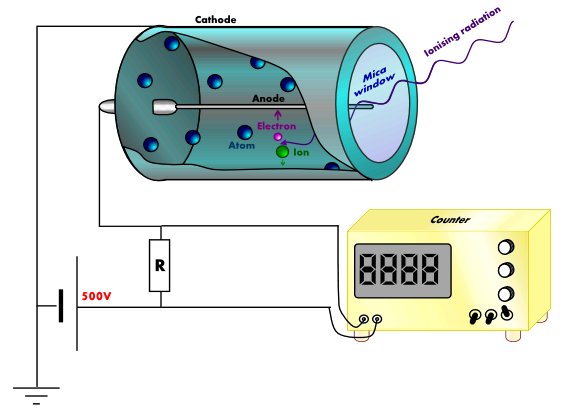
\includegraphics[width=4.5in]{immagini/geiger.jpg} %immagine
\end{center}

L'impulso elettrico risultante sarà testimone dell'avvenuto contatto con una radiazione ionizzante, e sarà contato da un circuito elettronico (i famosi “click” che si sentono). A seconda del numero di conteggi fatti in un'unità di tempo, riusciamo a capire se siamo in presenza di una sorgente radioattiva, e la sua pericolosità.

La dinamica di questi rivelatori è abbastanza ridotta, a causa del tempo morto durante il quale avviene un conteggio (ordine dei ms).

\subsection{Scintillatori} %Scintillatori
Lo \textbf{schema di funzionamento} è di questo tipo: lo scintillatore è connesso al fotomoltiplicatore attraverso una guida di luce; una particella che passa attraverso lo scintillatore perde energia trasferendola a quest'ultimo con meccanismi particolari cui segue poi l'emissione di fotoni. Negli scintillatori amorfi (plastici, liquidi), l'energia trasferita viene utilizzata per eccitarne le molecole che, poi, diseccitandosi emettono fotoni con un andamento temporale di tipo esponenziale.

\begin{center}
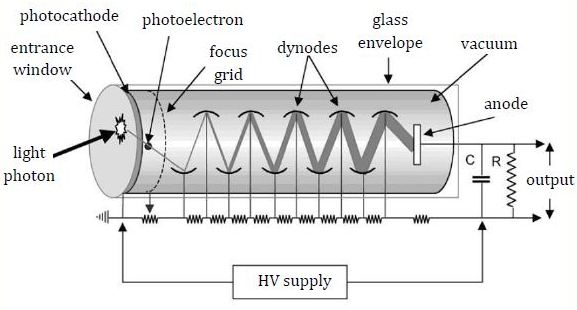
\includegraphics[width=4.5in]{immagini/scintillatore.jpg} %immagine
\end{center}

Negli scintillatori più comuni l'emissione avviene prevalentemente nel violetto, con tempi variabili dai \si{\nano\second} ai \si{\micro\second}. Tali fotoni sono poi trasmessi, attraverso una guida di luce opportuna, al fotocatodo del fotomoltiplicatore. Qui i fotoni liberano degli elettroni per effetto fotoelettrico che sono poi accelerati e focalizzati sul primo dinodo. \textbf{Il rapporto tra il numero dei fotoelettroni prodotti ed il numero di fotoni incidenti sul fotocatodo viene detto efficienza quantistica del fotocatodo}. Per ogni elettrone primario che urta un dinodo, possono essere emessi dai 2 ai 5 elettroni secondari. Introducendo, ad esempio, 14 stadi di moltiplicazione, si raggiungono fattori di moltiplicazione di circa un miliardo. La carica raccolta (integrale dell'impulso) e l'ampiezza degli impulsi sono proporzionali all'energia depositata nello scintillatore.

Gli scintillatori possono essere organici o inorganici (i quali hanno una migliore risposta di luce, ma sono più lenti nella risposta temporale rispetto a quelli organici).

Funzionano grazie ad un meccanismo per il quale degli atomi emettono una radiazione. La radiazione colpisce un materiale scintillante che emette cariche poi amplificate (da un fotomoltiplicatore). I \textbf{pregi degli scintillatori} sono:
\begin{itemize}
\item misura accurata dell'energia;
\item alta risoluzione temporale (lns);
\item possibilità di distinguere le particelle.
\end{itemize}

\subsection{Cherenkov} %Cherenkov
\textbf{Una particella passa attraverso un materiale ad una velocità maggiore di quella con cui la luce può viaggiare attraverso il materiale emette luce}. Questo è simile alla produzione di un boom sonico quando un velivolo viaggia attraverso l'aria più veloce di quanto le onde sonore possano muoversi attraverso l'aria. La direzione di questa luce viene emessa su un cono intorno alla direzione in cui la particella è in movimento.

\begin{equation}\begin{split}
c_{\textrm{mezzo}}=\frac{c}{n} \quad \quad \beta=\frac{1}{n} \\
\cos\left(\theta_c\right)=\frac{1}{\beta n}=\frac{c}{nv}
\end{split}\end{equation}

L'angolo del cono $\theta_c$ (indicando con $c$ velocità della luce nel vuoto e $n$ l'indice di rifrazione del mezzo) è una misura diretta della velocità della particella. La \textbf{formula di Frank-Tamm} $$\frac{\textrm{d}^2N}{\textrm{d} \omega \textrm{d}x} = \frac{z^2\alpha}{c} \sin^2 (\theta_c)$$ dà il numero di fotoni prodotti.

La maggior parte dei rivelatori Cherenkov mirano a registrare la luce Cherenkov prodotta da una particella carica primaria. Alcune tecnologie dei sensori mirano esplicitamente a luce Cherenkov prodotta (anche) da particelle secondarie, sia di emissione incoerente come si verifica in una elettromagnetica doccia di particelle o mediante emissione coerente, ad esempio per effetto Askaryan.

\textbf{La radiazione Cherenkov è presente non solo nel campo della luce visibile o luce UV ma anche in qualsiasi banda di frequenza in cui la condizione di emissione può essere soddisfatta cioè nel campo delle radiofrequenze}.

Diversi livelli di informazione possono essere utilizzati: un'informazione binaria può essere basata sulla presenza o l'assenza di radiazioni Cherenkov rilevate. Possono essere usati l'importo o la direzione della luce Cherenkov.

\textbf{In contrasto con un contatore a scintillazione la produzione di luce è istantanea}.

\paragraph{Tipi di rilevatori} Nel caso semplice di un \textbf{rivelatore di soglia}, l'energia di soglia massa-dipendente consente la discriminazione tra una particella più leggera (che irradia) e una particella pesante (che non irradia) della stessa energia o momento. Diverse fasi di soglia possono essere combinati per estendere la gamma di energia.

Utilizzando la direzione della luce sono stati creati i \textbf{rivelatori Cherenkov differenziali}.

\subsection{Camera a nebbia o di Wilson} %Camera a nebbia o di Wilson
Un rapido spostamento dello stantuffo provoca nella camera un'espansione adiabatica del vapore che passa allo \textbf{stato instabile di soprassaturazione}. In tali condizioni \textbf{una qualsiasi particella elementare carica elettricamente che penetri nella scatola ionizzando gli atomi con i quali si scontra crea, lungo il proprio tragitto, un fitto susseguirsi di nuclei di condensazione (atomi ionizzati), attorno ai quali il vapore soprassaturo si raccoglie a formare minuscole goccioline (nebbia)}.
La traccia lasciata dalla traiettoria percorsa della particella può essere fotografata attraverso una parete trasparente della scatola e da questa si può risalire, con particolari accorgimenti, alla determinazione della natura della particella.

Prima di ripetere il ciclo è opportuno rimuovere gli ioni attraverso un campo elettrico e rieffettuare la compressione.

Nelle camere a nebbia moderne lo scatto del pistone è comandato, con l'ausilio di un circuito elettronico, dall'arrivo stesso della particella da studiare.

\begin{center}
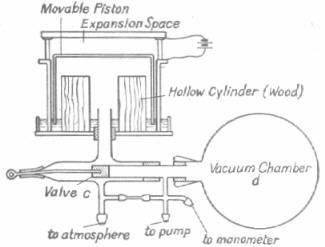
\includegraphics[width=4in]{immagini/wilson.jpg} %immagine
\end{center}

Simile per concezione alla camera a nebbia è la più moderna camera a bolle.

\subsection{Camera a bolle} %Camera a bolle
\textbf{La camera a bolle è costituita da un recipiente metallico cilindrico (di raggio pari a circa 5 m) contenente il liquido in condizione metastabile (surriscaldato e compresso)}.

Una particella carica veloce che attraversi il recipiente ionizza molti atomi del liquido, perdendo nel contempo parte della sua energia pur senza subire deviazioni apprezzabili. Lungo il percorso della particella vengono a trovarsi ioni positivi e negativi attorno a cui il liquido inizia a bollire e le bollicine che si creano possono ingrandirsi fino a riempire tutta la camera.

Usando un campo magnetico si può realizzare un ciclotrone dentro in contenitore ed ottenere informazioni su $E$ e su $p$.

\textbf{Rispetto ad altri rivelatori ha migliore risoluzione spaziale e temporale e miglior potere di frenamento anche per particelle leggere}.

Scattando diverse foto da angolazioni differenti, si ottiene una ricostruzione stereoscopica spaziale delle tracce.

\textbf{Per poter riutilizzare nuovamente la camera a bolle è necessario aumentare la pressione per far cessare l’ebollizione del liquido, per poi ripristinare la situazione metastabile}.

Solitamente una camera a bolle è circondata da un grosso magnete il cui campo magnetico, omogeneo in tutto lo spazio della camera, deflette le particelle cariche lungo una traiettoria circolare (ossia realizza un ciclotrone) il cui raggio dipende dalla quantità di moto delle particelle. Analizzando le tracce, si hanno informazioni sulla massa e sulla velocità delle particelle.

\begin{center}
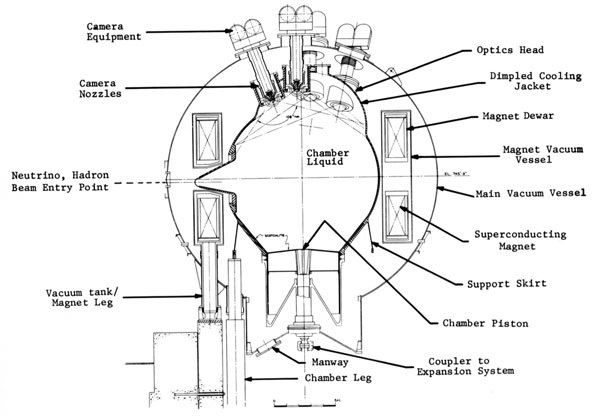
\includegraphics[width=\textwidth]{immagini/bolle.jpg} %immagine
\end{center}

\begin{center}
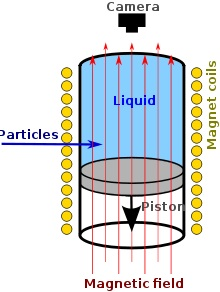
\includegraphics[width=2.6in]{immagini/camera_bolle.jpg} %immagine
\end{center}

Dal raggio di curvatura $R$ si ricava l’impulso della particella tramite la relazione seguente:
\begin{equation}\begin{split}
p(\si{MeV/c}) = 0,30\cdot B(\si{\kilo G})\cdot R(\si{cm})\cdot g
p(\si{GeV/c})=0,30\cdot B(\si{T})\cdot R(\si{m})\cdot g
\end{split}\end{equation}
essendo $g$ l'ingrandimento della fotografia.

Rispetto alla camera a nebbia la camera a bolle offre:
\begin{itemize}
\item densità maggiore e quindi: maggiore ionizzazione, migliore definizione delle tracce e migliore risoluzione spaziale;
\item tempo molto minore;
\item migliore potere di frenamento anche per particelle leggere o a bassa energia.
\end{itemize}

\subsection{Emulsioni nucleari} %Emulsioni nucleari
\textbf{Le emulsioni nucleari non sono altro che lastre fotografiche}. Se una particella carica attraversa una lastra fotografica lascia una traccia nella lastra ben visibile dopo lo sviluppo della lastra stessa.

L’emulsione consiste di cristalli di bromuro d’argento a piccoli grani ($\sim 0.25$ mm) immersi in una gelatina.

Esattamente allo stesso modo che per la luce la particella ionizzante produce dei cambiamenti chimici nei grani di bromuro d’argento. Durante lo sviluppo gli ioni d’argento del sale diventano atomi d’argento e la sequenza dei grani d’argento formano una traccia.

\textbf{Con questo metodo metodo non si ha risoluzione temporale ma si possono raggiungere precisioni fino ad 1 mm}.

\subsection{Camera a scintille} %Camera a scintille
Prima dello sviluppo delle camere proporzionali o a deriva venivano usate molto le camere a scintilla quali tracciatori. \textbf{Le camere a scintilla possono essere triggerate} (come le camere streamer).

Un insieme di piastre metalliche è inserito in un volume riempito di un gas nobile (generalmente un miscuglio di elio e neon) a pressione atmosferica.

Le piastre sono alternativamente poste ad alta tensione o a massa. Al passaggio di una particella ionizzante un trigger genera un impulso di alta tensione ( $\sim 20$ KV ) che viene inviato alle piastre (una sì ed una no). Il campo elettrico cosi generato fa sì che gli elettroni di ionizzazione formano valanghe e streamer. Le valanghe raggiungono gli elettrodi ed il segnale è o fotografato o raccolto elettronicamente.

\subsection{Camera streamer} %Camera streamer
\textbf{Le camere streamer sono delle grosse camere in cui gli eventi (tracce) sono normalmente fotografati}. In una camera streamer il volume fra due elettrodi planari è riempito di gas.

\textbf{Al passaggio di una particella carica, una grossa differenza di potenziale è applicata fra gli elettrodi}. Questa differenza di potenziale è limitata nel tempo.

Nelle applicazioni più comuni in genere la particella ionizzante attraversa la camera quasi ortogonale al campo elettrico. Ogni $e$ di ionizzazione primaria comincia una valanga che si muove verso gli elettrodi. Siccome il campo elettrico dipende dal tempo (ampiezza dell’impulso di alta tensione $\sim 50$ KV, tempo di salita e di discesa $\sim 1$ ns, durata dell’impulso parecchi ns) la formazione della valanga è interrotta non appena il campo elettrico finisce.

L’alto campo elettrico permette alti guadagni ($\sim 108$) come nei tubi streamer, ma le valanghe si estendono in una piccola regione dello spazio. Nel corso dello sviluppo della valanga molti atomi si eccitano ed emettono luce diseccitandosi. Si formano cosi dei puntini luminosi che vengono fotografati.

\chapter[Effetti biologici]{Effetti delle radiazioni sui sistemi biologici} %Effetti delle radiazioni sui sistemi biologici
\textbf{L'effetto biologico è dovuto in massima parte alle proprietà ionizzanti: distruggendo i legami fra molecole, le radiazioni danneggiano le cellule generando radicali liberi. Ma soprattutto alterano le grandi macromolecole del DNA e dell'RNA, causando danni somatici e genetici; tale effetto è prodotto principalmente dalle radiazioni $\gamma$}, più energiche e penetranti delle particelle $\alpha$ e $\beta$. Inoltre alterano le funzioni e gli apporti degli oligoelementi nel metabolismo organico.

Il momento in cui le cellule sono più vulnerabili in rapporto alle radiazioni, è quello della riproduzione (mitosi o meiosi), in cui il DNA è in fase di duplicazione, le strutture del nucleo sono dissolte e gli enzimi che assicurano l'integrità del materiale genetico non possono operare.

L'effetto macroscopico più vistoso della radioattività sulle cellule, quindi, è il \textbf{rallentamento della velocità di riproduzione}: le popolazioni di cellule che si riproducono molto rapidamente sono più vulnerabili di quelle che lo fanno lentamente. In virtù di questo fatto, gli organi più sensibili alle radiazioni sono il midollo osseo emopoietico e il sistema linfatico.

\textbf{A livello dell'intero organismo invece, sia nell'uomo che negli animali superiori si nota un precoce invecchiamento dell'organismo correlato alla dose totale di radiazione assorbita, sia con forti dosi istantanee che con l'esposizione prolungata a bassi livelli di radioattività}.

La ionizzazione dei tessuti provoca danni all'organismo ma anche la ionizzazione dell'acqua contenuta nel nostro organismo può provocare danni.

Un esempio è: $$\textrm{radiazione}+\ce{H2O}\longrightarrow e^-+\ce{H2O+}\longrightarrow \ce{H2O-}$$ dove sia \ce{H2O+} che \ce{H2O-} non sono stabili e formano uno ione e un radicale libero. $$\ce{H2O+} \longrightarrow \ce{H+} +\ce{OH}^*$$ $$\ce{H2O-} \longrightarrow \ce{H}^* +\ce{OH-}.$$ I radicali liberi hanno una forte tendenza a ricombinarsi con le altre molecole creando nuovi composti potenzialmente pericolosi sia in modo indiretto che diretto.

I diversi tipi di radiazioni hanno differenti caratteristiche di penetrazione:
\begin{itemize}
\item \textbf{gli $\alpha$ sono poco penetranti ma se un emettitore di $\alpha$ viene ingerito può essere molto dannoso};
\item \textbf{gli elettroni sono leggeri e facilmente diffondibili, più penetranti delle $\alpha$ e irradiano una zona più estesa, anche se depositano una minor densità di energia};
\item \textbf{i neutroni interagiscono coi nuclei}.
\end{itemize}

L'unità di misura della dose è il Gray. Un Gray è un Joule assorbito da un Kg di materia. La \textbf{dose equivalente} tiene conto anche della pericolosità della radiazione e ha come unità di misura il Sievert: $$1 \textrm{ Sv} = 1 \textrm{ Gy}\cdot Q$$ indicando con $Q$ il fattore di qualità.

\textbf{La stessa dose di radiazione può avere differenti pericolosità in base al suo tipo, mentre la dose equivalente tiene conto anche a quale tipo di radiazione sia}.

Il tempo di assorbimento della radiazione è importante in quanto la stessa dose assorbita in un tempo più lungo fa meno male (ovviamente gli effetti dipendono anche dal tipo di tessuto). Le modifiche alle cellule possono avere effetti a breve o a lungo termine.

Gli effetti delle radiazioni ionizzanti si suddividono in \emph{effetti deterministici} ed \emph{effetti stocastici}, a seconda se sono correlati direttamente o meno alla dose assorbita. Per via della suscettibilità al cancro al seno, le donne hanno un 40\% di probabilità in più di accusare effetti stocastici rispetto agli uomini.

\paragraph{Effetti deterministici} %Effetti deterministici
\begin{itemize}
\item Sono attribuibili direttamente all'irraggiamento (c'è una relazione diretta causa-effetto);
\item Derivano dalla inattivazione delle strutture vitali della cellula;
\item Si manifestano subito dopo l'irradiazione;
\item Si manifestano solo se l'assorbimento supera una dose ben precisa detta \textbf{dose soglia};
\item La loro gravità cresce al crescere della dose assorbita (perciò detti anche ``effetti graduati'').
\item Gli effetti deterministici sono eritemi cutanei, particolari dermatiti (dermatiti da radiazioni appunto), cataratta, anemia e leucopenia. Nei casi più gravi si hanno emorragie delle mucose e del tratto intestinale, perdita di capelli e peli. Se la dose assorbita non era letale, gli effetti deterministici regrediscono nel giro di alcune settimane, con sopravvivenza e guarigione più o meno completa.
\end{itemize}

\paragraph{Effetti stocastici} %Effetti stocastici
\begin{itemize}
\item Non dipendono dalla dose assorbita;
\item Derivano da danni al nucleo cellulare e in particolare al DNA;
\item Non si manifestano subito; possono verificarsi o meno, in un futuro imprecisato;
\item Dopo l'irraggiamento, il DNA potrà essere danneggiato in maniera reversibile o irreversibile; nel caso in cui la struttura del DNA non venisse riparata (o riparata in modo errato) la cellula darebbe vita a una progenie di cellule geneticamente modificate che dopo un certo periodo di latenza potranno dar luogo a patologie come tumori o leucemie. Aumenta pertanto la probabilità che il paziente, prima o poi, venga colpito da certi tipi di tumore.
\end{itemize}

\section{Efficacia di una radiazione ionizzante} %Efficacia di una radiazione ionizzante
Gli effetti dell'irradiazione di un tumore non dipendono solo dall'entità di dose assorbita che esprime a livello macroscopico la cessione locale di energia, ma bisogna tener conto di altri tre parametri:

\begin{itemize}
\item \textbf{il primo parametro è il LET (Linear Energy Transfer)} definito come rapporto fra la quantità di energia ($\Delta E$) rilasciata da una particella carica e lo spessore ($\Delta x$) di tessuto entro cui questa energia viene rilasciata, si può esprimere come: 
\begin{equation}
\textrm{LET}=\frac{\Delta E}{\Delta x} (\si{KeV/\micro m}).
\end{equation}

Questo valore dipende dall'energia e dalla carica della particella. Infatti il LET di protoni e ioni pesanti a fine percorso è decisamente più elevato rispetto a quello dei fasci convenzionali di fotoni ed elettroni. Perciò i primi risultano più efficaci nel trattamento di neoplasie. Per gli elettroni è di pochi keV; per gli $\alpha$ è di qualche centinaio di keV.

L'entità del danno ai tessuti dipende dall'energia assorbita:
\begin{equation}
\textrm{\textbf{dose}}=\frac{\textrm{energia assorbita}}{\textrm{massa}}.
\end{equation}


\item \textbf{il secondo parametro è l'OER (Oxygen Enhancement Ratio)} che rappresenta il rapporto tra la dose necessaria ($D$) per produrre un dato effetto nel tessuto cancerogeno e ($D_0$) la dose che produrrebbe lo stesso risultato se il tessuto fosse completamente ossigenato, si può scrivere come:
\begin{equation}
\textrm{OER}=\frac{D}{D_0}.
\end{equation}

\textbf{L'efficacia della radiazione aumenta quanto più il valore di tale rapporto è prossimo a 1}. L'OER dunque è il parametro che ci permette di quantificare la correlazione esistente fra contenuto di ossigeno nei tessuti irradiati ed effetti biologici indotti dalla radiazione. Infatti nei tessuti tumorali scarsamente vascolarizzati il contenuto di ossigeno è generalmente basso, ed è proprio in queste condizioni che gli effetti biologici dovuti alla produzione di perossidi organici, di elevata tossicità per le bio-molecole coinvolte, diminuiscono.

Inoltre tale parametro può essere considerato una funzione decrescente del LET in quanto fasci di particelle a basso LET hanno elevati valori di OER e viceversa. Questo significa che \textbf{radiazioni altamente ionizzanti, come protoni e ioni leggeri, agiscono in modo pressoché equivalente sia in eccesso che in difetto di ossigeno e perciò sono più indicate rispetto a fotoni ed elettroni nella trattazione di cellule ipossiche come quelle tumorali nella zona della necrosi}.

\item \textbf{il terzo parametro è l'RBE (Relative Biological Effectiveness)} il quale è definito come il rapporto tra la dose assorbita ($D_{\gamma}$) necessaria a produrre un determinato effetto nel sistema irradiato con il fascio di riferimento fotonico, e la dose ($D$) che produce il medesimo risultato con una determinata radiazione, per esempio protonica. Si può esprimere come: 
\begin{equation}
\textrm{RBE}= \frac{D_{\gamma}}{D} (\si{Sv^2}).
\end{equation}

Esiste una relazione funzionale anche tra questo parametro e il LET secondo la quale, nella regione di LET relativa agli adroni l'RBE è una funzione crescente del LET e ciò indica che \textbf{le radiazioni densamente ionizzanti hanno maggior effetto biologico}.
\end{itemize}

\section{Medicina nucleare} %Medicina nucleare
Si usano i decadimenti nucleari e le radiazioni emesse sia a scopi diagnostici che terapeutici che nella ricerca in campo biomedico.

Vengono definiti \textbf{radionuclidi} delle molecole radiomarcate introdotte nell'organismo (soluzioni, sospensioni o aerosol) usati come traccianti oppure attraverso bombardamenti possono essere distrutte delle parti. Attraverso opportuni rivelatori si possono produrre immagini diagnostiche grazie al tracciamento dato dai radionuclidi.

Con le normali analisi radiologiche a raggi X si sfrutta l'attenuazione di intensità mentre le immagini medico-nucleari vengono ottenute dalle radiazioni emesse dai radiofarmaci distribuiti nell'organismo (ruolo attivo dell'organo). La radiazione emessa dall'organo viene restituita sotto forma di immagine. I raggi X vengono utilizzati per le radiografie utilizzando la proprietà di queste radiazioni di penetrare in modo diverso i tessuti con minor o maggiore densità.

L'immagine ottenuta (ad esempio la \textbf{scintigrafia}) viene creata trasformando l'energia quantistica in energia elettrica. La scelta del radiofarmaco è fatta in base alle circostanze ed in modo che questo si possa concentrare nell'organo che si vuole studiare. Le immagini scintigrafiche danno distribuzione spaziale o spazio-temporale dei radiofarmaci (minor dettaglio morfologico ma maggiori informazioni dal punto di vista funzionale). L'immagine scintigrafica evidenzia ``malfunzionamenti'' anche prima che ci siano alterazioni morfologiche.

Altro utilizzo dei radiofarmaci è quello di distruggere certi tessuti in modo quanto più possibile selettivo.

Si ha un rilascio di energia in spazi piccoli (meno di 1 cm): \textbf{terapia metabolica}.

La diagnostica per immagini rappresenta le funzioni biochimiche e fisiologiche dell'organismo e avviene attraverso questi passaggi:
\begin{itemize}
\item preparazione radionuclidi;
\item diffusione dei radionuclidi nell'organismo;
\item decadimento dei radionuclidi;
\item attenuazione della radiazione nella materia biologica;
\item rilevazione e elaborazione immagini.
\end{itemize}

\paragraph{Tomografie:} consentono di riprodurre sezioni dell'organismo studiato, esempio TAC che sfrutta i raggi X per fare immagini in 3D (la ``C'' di TAC sta per computer), però la dose è superiore a quella di una radiografia.

C'è anche la \textbf{SPET (Single Photon Emitted Tomography)} o la \textbf{SPECT} (la ``C'' sta per computer): il rivelatore consiste di una o più fotocamere ruotate attorno all'organismo in modo da generare l'immagine 3D. La risoluzione dipende da molti fattori sia fisico-nucleari che biologici. Il tempo per produrre l'immagine è alto: per immagini rapide è meglio la PET

\paragraph{Positron Emission Tomography (PET):} emissione di radioisotopo che emette elettrone e positrone che annichilano e danno due fotoni $\gamma$.

La PET usa radionuclidi che decadono $\beta^+$, permettendo di marcare le molecole biologiche sostituendo le molecole stabili con radioattive (non modifica le cellule perché si usano dei radionuclidi con caratteristiche simili fra i vari isotopi).

Avviene seguendo questo processo: si somministrano piccole dosi $\longrightarrow$ decadimento $\beta^+$ $\longrightarrow$ emissione positroni $\longrightarrow$ annichilazione (applicazione usata soprattutto nelle attività cerebrali).

Esiste una terapia di cattura di neutroni da parte del boro: \textbf{BNCT} $$\textrm{neutrone} + \ce{^10B} \longrightarrow \ce{^11B}$$ si formano neutroni termici che formano il boro-11 che può o decadere $\alpha$ al (6.1\%) oppure si forma uno stato eccitato (93.9\%) che poi decade ed emette un $\gamma$ da 0.478 MeV rilasciando energia ad una distanza di pochi \si{\micro m} dal punto in cui sono stati creati.

A basse energia l'$\alpha$ ha alte capacità distruttive, perciò si fa assorbire selettivamente dalle cellule cancerogene il radiofarmaco che quando emetterà $\alpha$ le distruggerà (si bombarda con elettroni e si distruggono solo le cellule che contengono il radiofarmaco: è molto selettivo). \textbf{La dose viene rilasciata solo durante l'irraggiamento}, i prodotti delle reazioni non sono radioattivi. Il resto del corpo non riceve dosi di radiazioni.

A Pavia c'era il progetto \textbf{TAORMINA} per tumori al fegato: espianto temporaneo del fegato che viene poi bombardato in un reattore senza coinvolgere il paziente. Le $\alpha$ distruggono le cellule tumorali. Poi l'organo viene reimpiantato. All'inizio degli anni duemila sono stati effettuati due esperimenti: il primo paziente ha vissuto ancora un mese il secondo paziente ha vissuto per altri 44 mesi. Ora non sono più autorizzati esperimenti.

\paragraph{Adroterapia:} (usa adroni, cioè particelle con interazione nucleare forte) si usano ioni ad esempio di carbonio. Se delle particelle cariche attraversano un mezzo cedono energia per interazione coulombiana. \textbf{Le particelle neutre hanno un rilascio di energia esponenziale mentre quelle cariche hanno un rilascio tipo curva di Bragg (l'emissione di energia è concentrata in una regione ristretta alla fine del cammino)}.

Quando un adrone carico entra nella materia viene rallentato e al diminuire della sua energia le probabilità di urto aumentano. Si può andare a fondo in modo mirato variando l'energia delle particelle. Si possono mirare bene le cellule malate, anche in tessuti profondi, risparmiando le cellule sane (vengono usati ioni di \ce{C} oppure protoni).

Il vantaggio degli ioni di carbonio è che il LET è maggiore rispetto ai protoni (maggior probabilità di colpire e danneggiare e minore dispersione laterale). Nel carbonio però c'è una coda più grande dopo il picco rispetto ai protoni. \textbf{L'adroterapia non sostituisce le altre terapie, dipende dai casi}.

\chapter{Applicazioni} %Applicazioni

\section[Metodo del $\ce{^{14}C}$]{Metodo del carbonio-14 $\ce{^{14}C}$} %Metodo del C14
Il metodo del \ce{^{14}C} (carbonio-14), o del radiocarbonio, è un metodo di datazione radiometrica basato sulla misura delle abbondanze relative degli isotopi del carbonio.

Fu ideato e messo a punto tra il 1945 e il 1955 dal chimico statunitense Willard Frank Libby, che per questa scoperta vinse il Premio Nobel nel 1960.

\textbf{Il metodo del \ce{^{14}C} permette di datare materiali di origine organica (ossa, legno, fibre tessili, semi, carboni di legno, ...). Si tratta di una datazione assoluta, vale a dire in anni calendariali, ed è utilizzabile per materiali di età compresa tra i \si{50.000} e i 100 anni. La sua principale utilizzazione è in archeologia per datare i reperti costituiti da materia organica, quindi contenenti atomi di carbonio}.

Il carbonio è un elemento chimico fondamentale per la vita e presente in tutte le sostanze organiche. Esso è presente sulla terra in tre isotopi: due stabili (\ce{^{12}C} e \ce{^{13}C}) e uno radioattivo (\ce{^{14}C}). Quest'ultimo si trasforma per decadimento $\beta$ in azoto (\ce{^{14}N}), con un tempo di dimezzamento medio (o emivita) di \si{5.730} anni, di conseguenza questo isotopo a lungo andare scomparirebbe, se non venisse continuamente reintegrato. La produzione di nuovo \ce{^{14}C} avviene regolarmente in natura negli strati alti della troposfera e nella stratosfera, per la cattura di neutroni termici componenti secondari dei raggi cosmici da parte degli atomi di azoto presenti nell'atmosfera. L'equilibrio dinamico che si instaura tra produzione e decadimento radioattivo mantiene quindi costante la concentrazione di \ce{^{14}C} nell'atmosfera, dove è presente principalmente legato all'ossigeno sotto forma di anidride carbonica.

\textbf{Tutti gli organismi viventi che fanno parte del ciclo del carbonio scambiano continuamente carbonio con l'atmosfera attraverso processi di respirazione (animali) o fotosintesi (vegetali), oppure lo assimilano nutrendosi di altri esseri viventi o sostanze organiche}.

Di conseguenza \textbf{finché un organismo è vivo, il rapporto tra la sua concentrazione di \ce{^{14}C} e quella degli altri due isotopi di carbonio si mantiene costante e uguale a quella che si riscontra nell'atmosfera}. Dopo la morte, però, questi processi terminano e l'organismo non scambia più carbonio con l'esterno. Per effetto del decadimento, quindi, la concentrazione di \ce{^{14}C} diminuisce in modo regolare secondo la formula:
\begin{equation}\begin{split}
c=c_0e^{-\frac{\Delta t}{\tau}}
\end{split}\end{equation}
dove $c_0$ è la concentrazione di \ce{^{14}C} nell'atmosfera, $\Delta t$ il tempo trascorso dalla morte dell'organismo, $\tau$ la vita media del \ce{^{14}C} (pari al tempo di dimezzamento diviso per il logaritmo naturale di 2: $\frac{5730}{\ln(2)} = \si{8.267}$ anni).

\textbf{Misurando dunque la quantità di \ce{^{14}C} presente nei resti organici, se ne ricava l'età applicando la seguente formula}:
\begin{equation}\begin{split}
\Delta t=-\tau\ln{\left(\frac{c}{c_0}\right)}
\end{split}\end{equation}

Accumuli naturali di carbonio di origine organica con età valutabile nella scala dei tempi geologici, quali i carboni fossili, risultano privi di \ce{^{14}C}, essendo questo ormai completamente decaduto in azoto.

La misura del \ce{^{14}C} si può effettuare con due metodi:
\begin{itemize}
\item \textbf{metodo del contatore proporzionale}: con un contatore Geiger o altra apparecchiatura simile si misurano gli elettroni prodotti dal decadimento del \ce{^{14}C} nel campione. Questo è stato il primo metodo ad essere impiegato;
\item \textbf{metodo della spettrometria di massa (AMS, Accelerator Mass Spectrometry)}: utilizzando uno spettrometro di massa si misura direttamente la concentrazione di \ce{^{14}C} presente nel campione. Questo metodo è di applicazione più recente, usato a partire dagli anni '70.
\end{itemize}

Rispetto al metodo del contatore proporzionale, il metodo AMS presenta il vantaggio di poter lavorare con campioni più piccoli (anche di pochi mg) e di fornire un risultato in un tempo molto più breve (si possono misurare decine di campioni al giorno, mentre il contatore proporzionale può richiedere anche alcune settimane per un solo campione). Tuttavia presenta anche lo svantaggio di essere un metodo distruttivo: esso richiede infatti che il campione venga bruciato e ridotto in forma gassosa.

Entrambi questi metodi permettono di ottenere datazioni con un margine di errore tra il 2 e il 5\% e fino ad un tempo massimo di circa \si{50.000} anni: per campioni più antichi, la concentrazione di \ce{^{14}C} è troppo bassa per poter essere misurata con sufficiente accuratezza.

\textbf{Il vantaggio delle radiazioni nucleari è che possono essere rivelate facilmente}. Per questo esiste lo studio di sistemi con traccianti radioattivi (medicina, agricoltura per studio distribuzione pesticidi oppure trasferimenti di minerali nella catena alimentare).

\textbf{In natura esistono più di 50 elementi con isotopi radioattivi con un neutrone in più} per questo si deve utilizzare una tecnica per misurare la concentrazione di certi elementi in materiali irraggiati da un fascio di neutroni. Essa è l'\textbf{analisi di attenuazione neutronica}.

\end{document}